\section{EVALUATION}
\label{sec:eva}
The proposed algorithm for platonic solids path planning by rolling through edge contact was implemented in MATLAB environment. 
In general of path planning, there are three case studies including same location and different orientation between initial configuration and goal configuration, long distance between two configurations, and bi-direction path-finding. 
To validate the proposed algorithm, this study only considers the first case study of path planning that both initial and goal configuration have the same positions and different orientations.\\  

\noindent Assume that the platonic solids' edges have the same length with $a$ ($a=1$) and one of the faces of the platonic solids contact to $OXY$. 
The environment for each type of platonic solids is discretized from the smooth surface. 
For example, cube solid will roll on the square grid while tetrahedron, octahedron, and icosahedron solids roll on the triangle gird. 
Only dodecahedron solid rolls on the pentagon grid with the two specific cases including the gaps and overlaps between pentagons. 
The path planning based on rolling for the five cases of platonic solids is represented as the following. 

\subsection{Cube solid}
\noindent\uline{Properties}:
The cube has a length $a$ which is the same as the length of the side of each grid square.
Path planning for rolling a cube is not as complex as other cases of platonic solids. 
The rolling angle $\beta$ has the value of $\frac{\pi}{2}$ as shown in Figure \ref{fig:cubeGeo1} ($\beta=\angle{IKI_1}=\frac{\pi}{2}$). 
The center of cube will move along the curve $II_2I_1$ following the $Ox$ axis. 
The proposed algorithms will focus on rolling along $Ox$ or $Oy$ axis. 
However, all the vertices are stored in a matrix will change their coordinates in $3D$ space. 
An example from the Figure \ref{fig:cubeGeo1}, eight vertices of the cube $ABCDMNOP$ and the center $I$ are stored in a matrix $M(9,3)$ with $9$ rows for nine $3D$ points, and $3$ columns for $3D$ coordinate $Ox,Oy,Oz$ of each point. 
After finishing the rotation angle $\beta$ based on the rotation axis $MN$, the coordinates of the cube's vertices are updated within a new cube $MA'D'PN'B'C'O'$. 
This is the basic step of rolling a cube through a line contact.

\begin{figure}[H]
\centering
	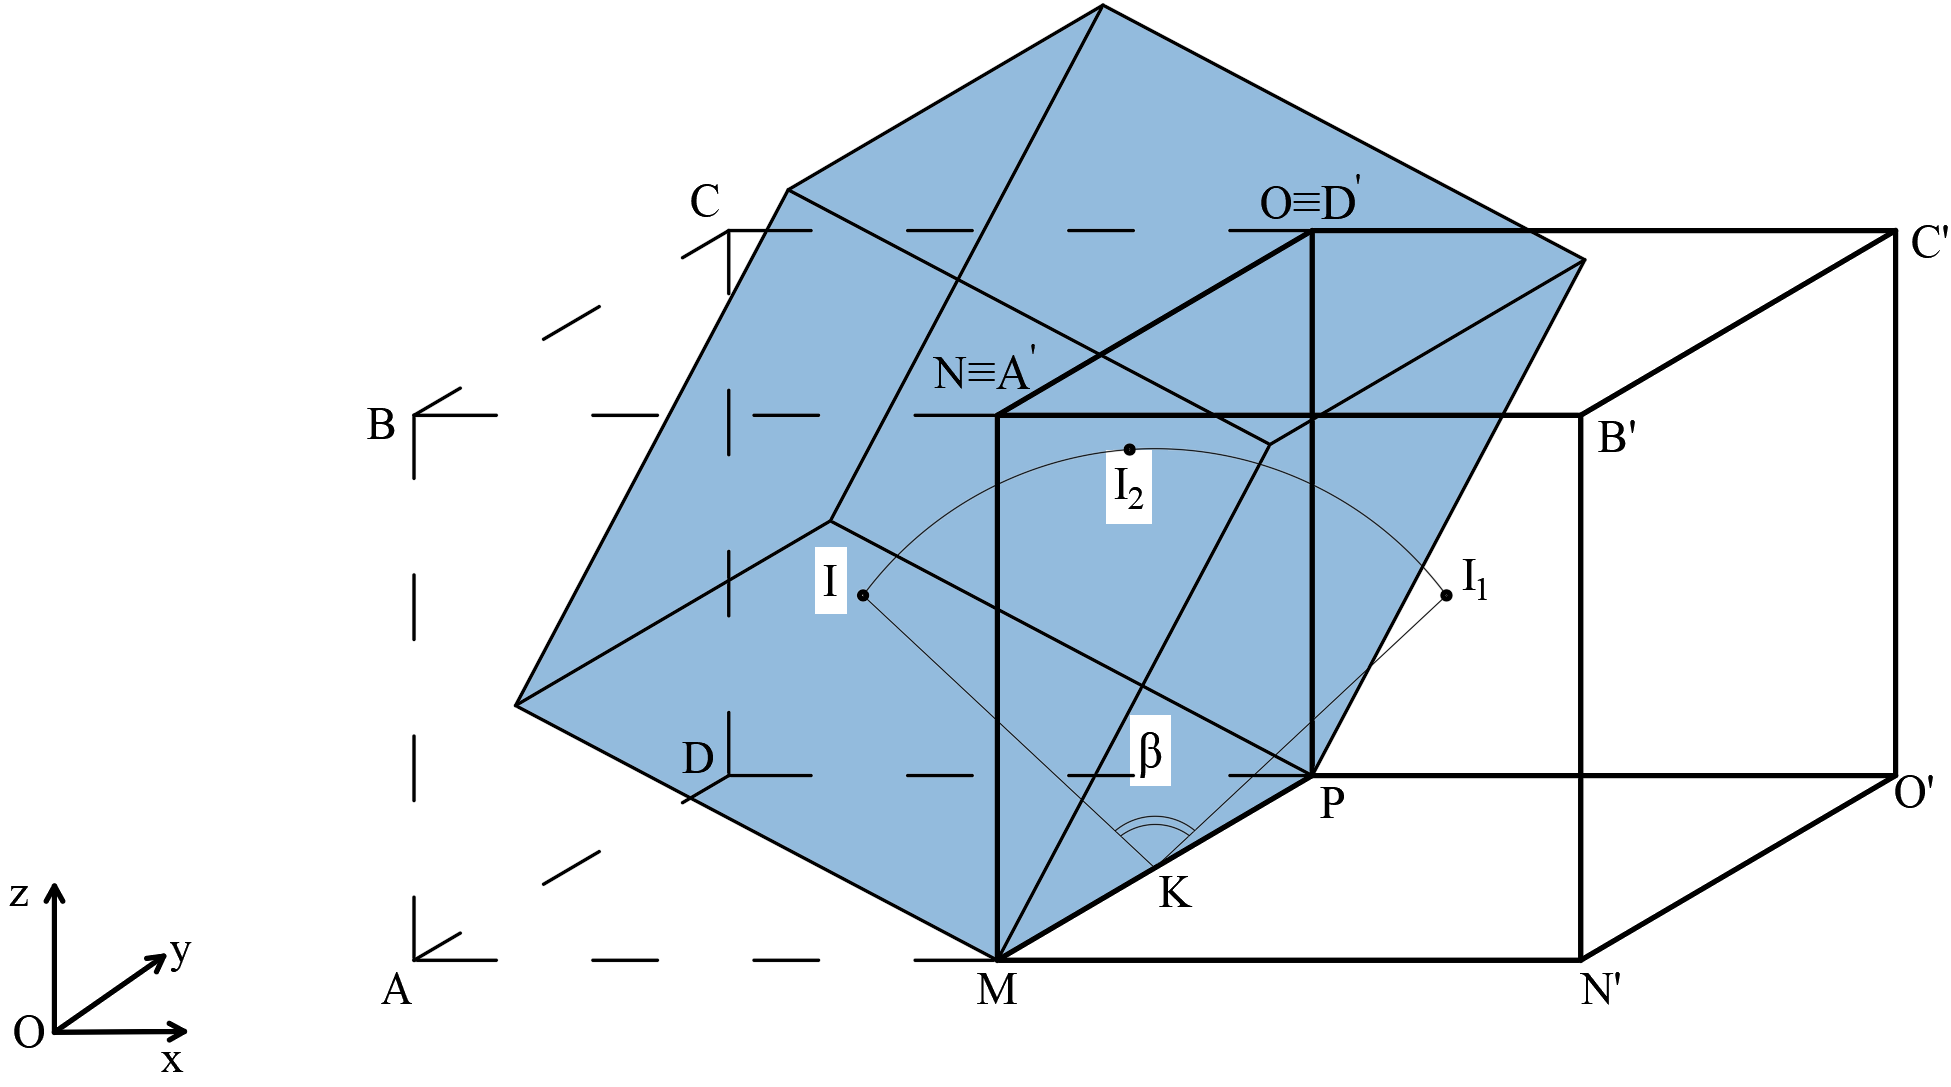
\includegraphics[width=1\textwidth]{image/cubeGeo1.png}
	\caption{Rotation angle of a cube on a plane}
	\label{fig:cubeGeo1}
\end{figure}

\noindent\uline{Path planning}: 
The only way to move from the initial position to the goal position of the cube solid is by rolling from square to square on the grid without moving diagonal. 
Figure \ref{fig:cubeLayer} shows the first four layers of the cube path-finding on the grid. 
The algorithm implements in $O(|E|^3)$ running time from the second layer called the expansion three branches from a tree. 
All $3D$ coordinates of the cube are stored in a matrix which can affect the computer's storage capacity. 
When the updated cubes achieved one of the same previous configurations, the execution time can be reduced by releasing this configuration or stopping the expansion of this tree branch.
The star position ($*$) in the grid (Figure \ref{fig:cubeLayer}) is occupied by the two updated cubes with different orientations in $Layer\ 2$. \\

\begin{figure}[H]
\centering
	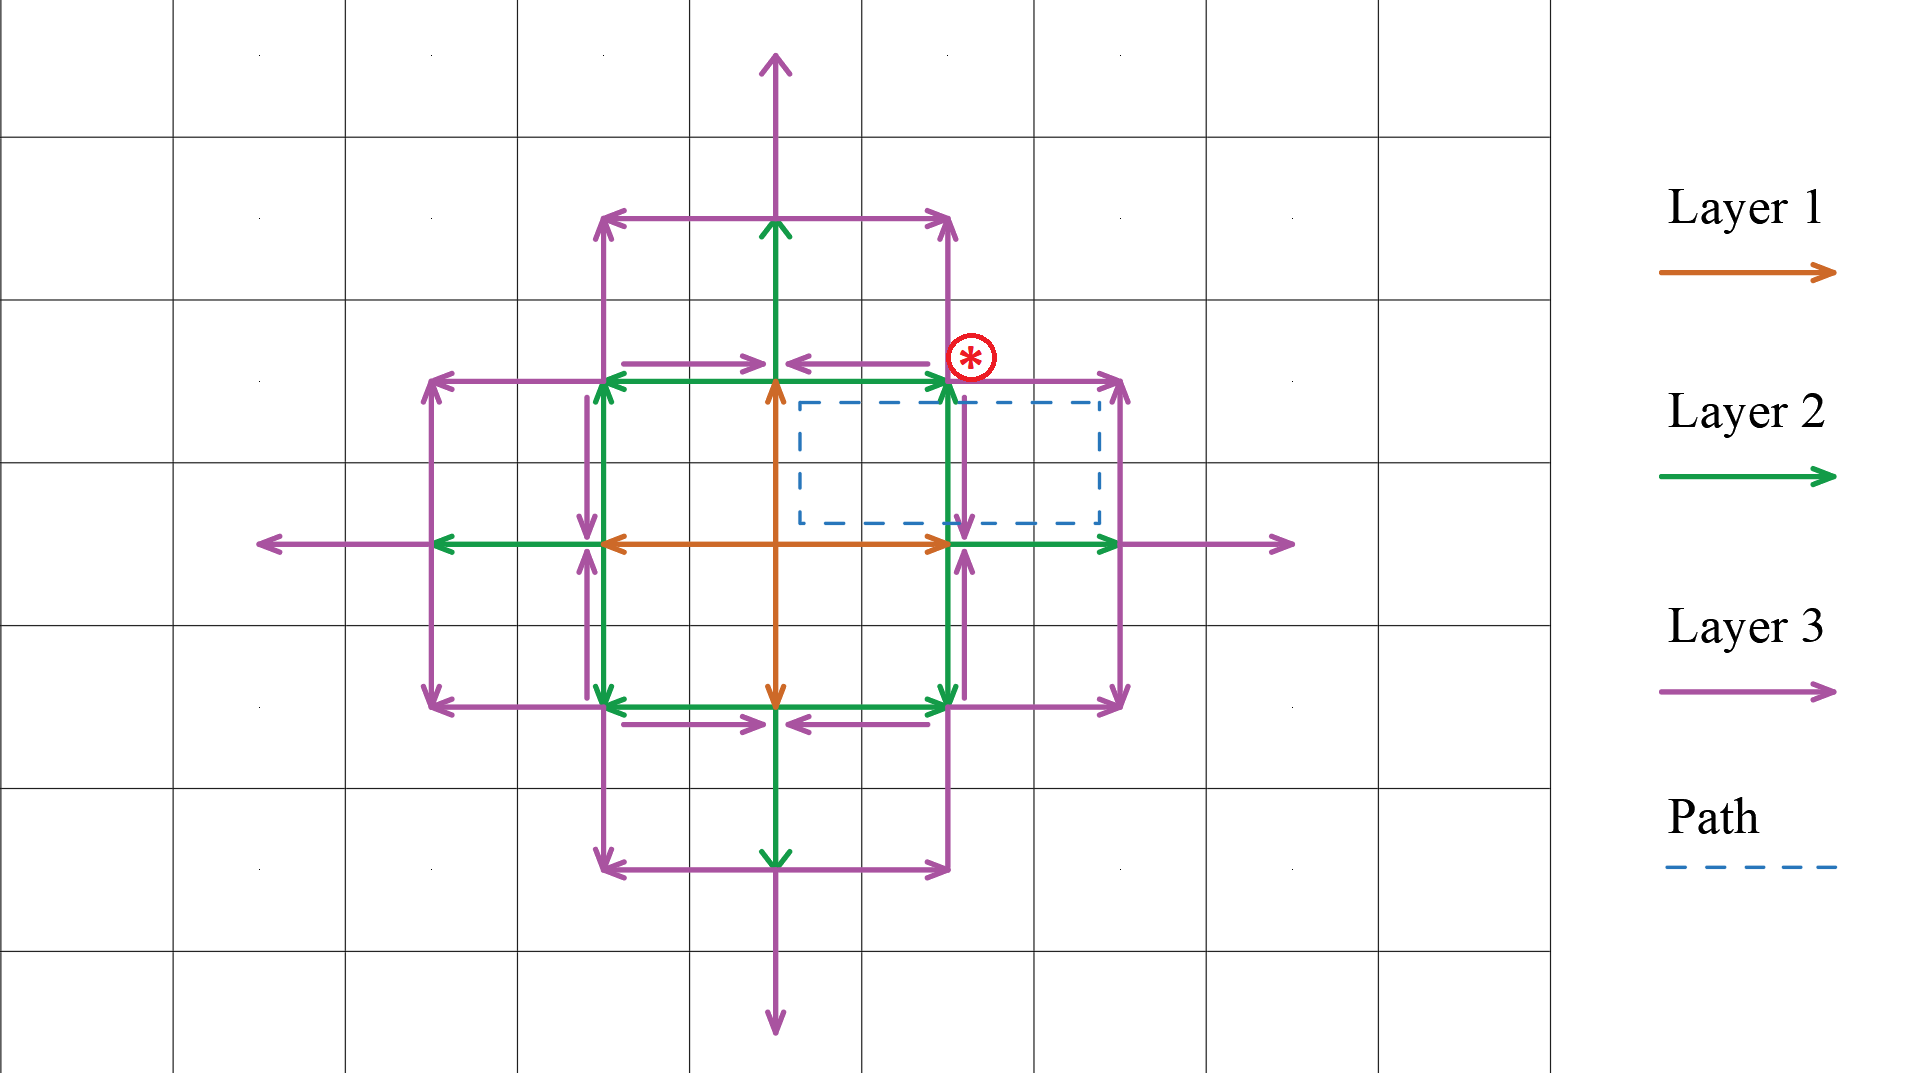
\includegraphics[width=1\textwidth]{image/cubePath00.png}
	\caption{The first four layers of cube rolling}
	\label{fig:cubeLayer}
\end{figure}
%
% ========================= Rodrigues Rotation Matrix

%
\noindent \uline{Rotation matrix}: 
In this paper, the Rodrigues' rotation matrix \cite{Dai_Rodrigues_2015} is used in each level of the proposed path planning algorithm to rotate the polyhedrons from a position to other positions.
%
In the $3D$ coordinate system, the unit vector is given by $\hat{\omega}=(\omega_x,\omega_y,\omega_z)\in{\textbf{R}^3}$.
The Euler-Rodrigues' rotation formula can be written in a standard form and then expressed as the $[3\times3]$ rotation matrix from the axis-angle representation of rotations as below.
%\textbf{R}{\_}{\hat{\omega}(\theta)} &= \textit{e^{\omega\theta}}\\
\begin{equation}
\begin{split}
R_{\hat{\omega}(\theta)} &= {e^{\omega\theta}}\\
	&= I + \omega\sin{\theta} + {\omega}^2(1-\cos{\theta})\\
	&= {
		\begin{bmatrix}
			{\cos{\theta}+{\omega_x}^2(1-\cos{\theta})} & {\omega_x\omega_y(1-\cos{\theta})-\omega_z{\sin\theta}} & {\omega_y\sin{\theta}+\omega_x\omega_z(1-\cos{\theta})}\\
			{\omega_z\sin{\theta}+\omega_x\omega_y(1-\cos{\theta})} & {\cos{\theta}+{\omega_y}^2(1-\cos{\theta})} & {-\omega_x\sin{\theta}+\omega_y\omega_z(1-\cos{\theta})}\\
			{-\omega_y\sin{\theta}+\omega_x\omega_z(1-\cos{\theta})} & {\omega_x\sin{\theta}+\omega_y\omega_z(1-\cos{\theta})} & {\cos{\theta}+{\omega_z}^2(1-\cos{\theta})}
		\end{bmatrix}
		}
\end{split}
\end{equation}

where \textbf{I} is the $3\times3$ identity matrix, and the $\omega$ denotes the antisymmetric matrix 

\begin{equation*}
\begin{split}
\omega &= {
		\begin{bmatrix}
			\omega\times
		\end{bmatrix}
		}
		= {
		\begin{bmatrix}
			0 & -\omega_z & \omega_y \\
			\omega_z & 0 & -\omega_x \\
			-\omega_y & \omega_x & 0
		\end{bmatrix}
		}
\end{split}
\end{equation*}

\noindent The matrix $\omega$ gives Lie algebra $so(3)$ in the form of a skew-symmetric matrix with the rotation matrix $\textbf{R}\in SO(3)$, which corresponds to a rotation angle $\theta$.
All the vertices' coordinates of the polygons will be stored in a matrix $A$ and a new matrix $A'$ is the product of $A$ and $\textbf{R}$ (Eq. \ref{equa:rotMatrix}). 
One of the edges of the polyhedrons which contacts the surface is considered as a rotation matrix.
For each iteration of the closed-path planning algorithm, it is essential to determine a direction and an edge of the polyhedrons before performing the rotation matrix to transform the polyhedron into a new configuration.
%
\begin{equation}
\begin{split}
A' = AR_{\hat{\omega}(\theta)}
\end{split}	
\label{equa:rotMatrix}
\end{equation}

where $A(m,n)$ is the matrix of $m$ rows for vertices and $n$ columns for $3D$ coordinates each vertex. The updated matrix is $A'(m',n')$ .\\

%
% =========================the paths ==================
%
\noindent To be more visualized, Figure \ref{fig:Cube1Case1} shows the initial configuration and the first step of rolling the cube with its coordinates in the red, green and blue arrows. 
The expansion of the cube after running the algorithm six iterations are shown in Figure \ref{fig:Cube2Case1}. 

\begin{center}
\begin{figure}[H]
\subfigure[The initial and goal configuration are initialized with the same position and different orientation]{
	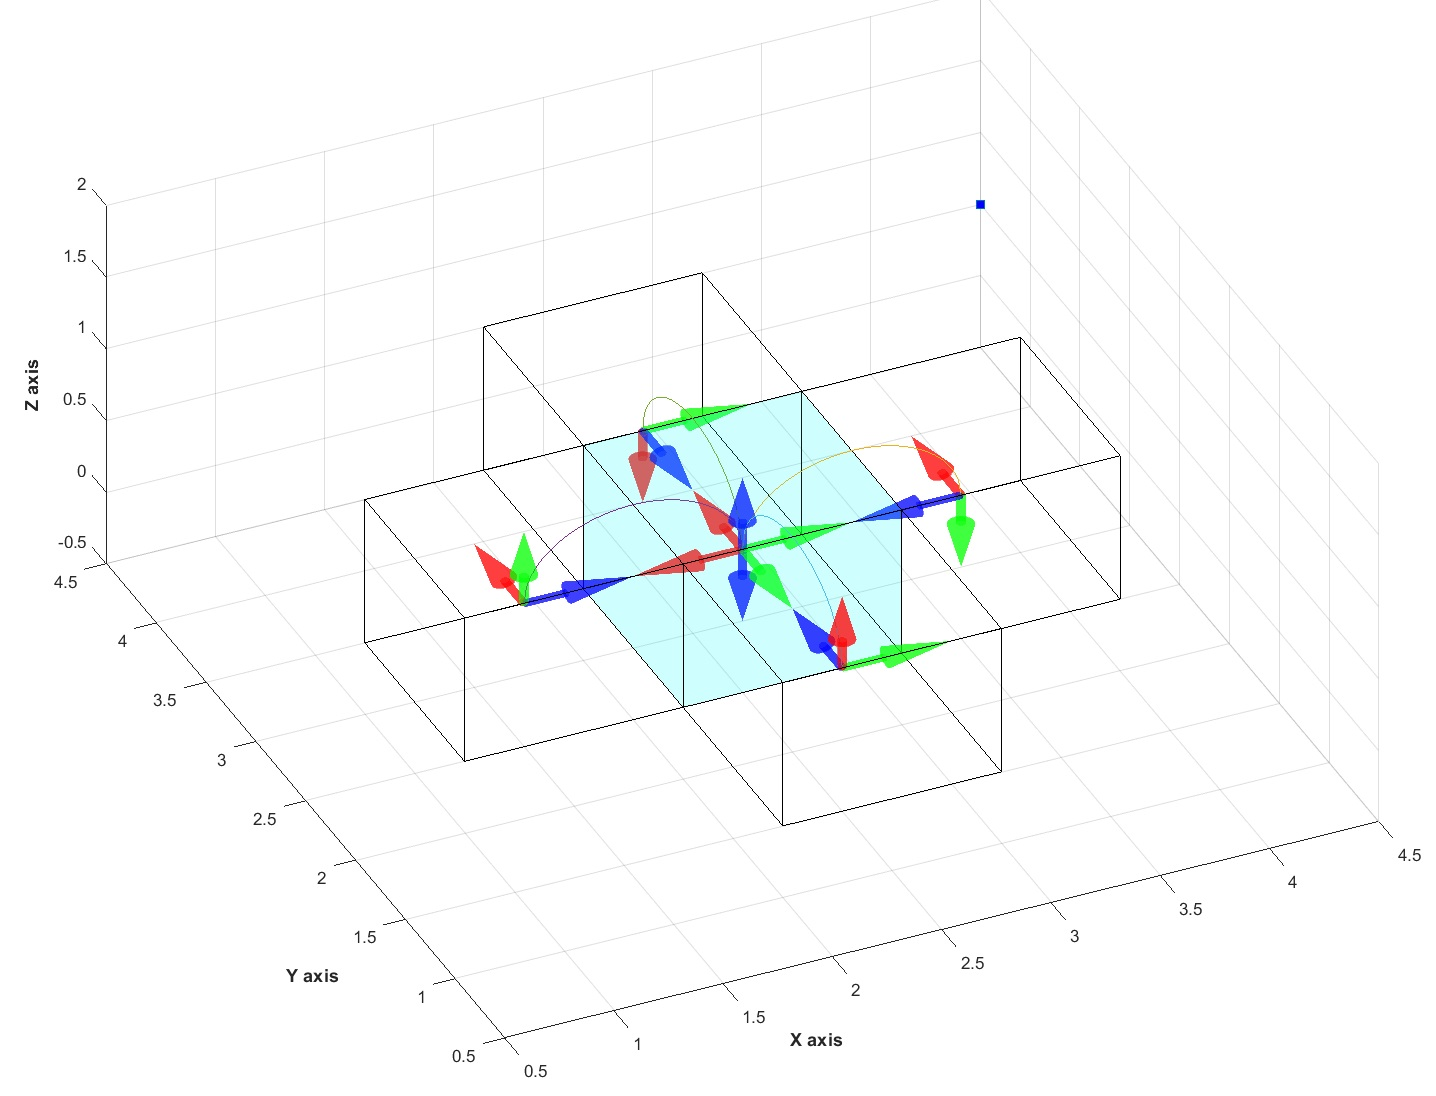
\includegraphics[width=0.5\textwidth]{image/cube11.jpg}
	\label{fig:Cube1Case1}
	}
\hfill
%\subfigure[First four paths of the cube rolling]{	
%	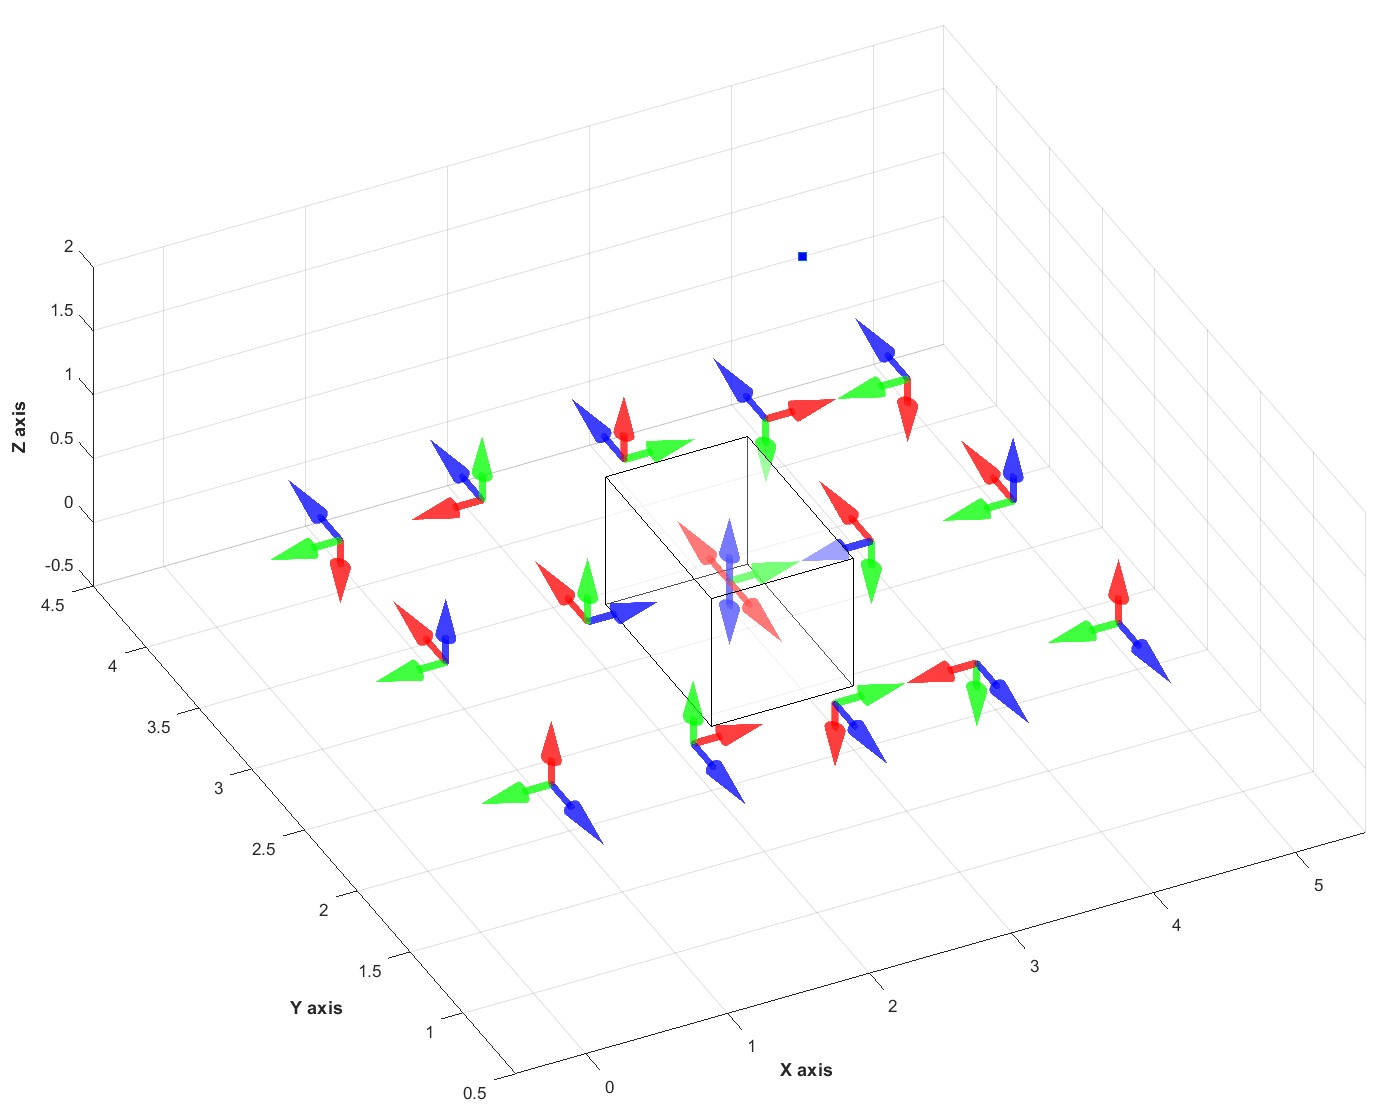
\includegraphics[width=0.5\textwidth]{image/cubePath4Dirs.jpg}
\subfigure[The expansion of cube rolling at $6^{th}\ level$]{
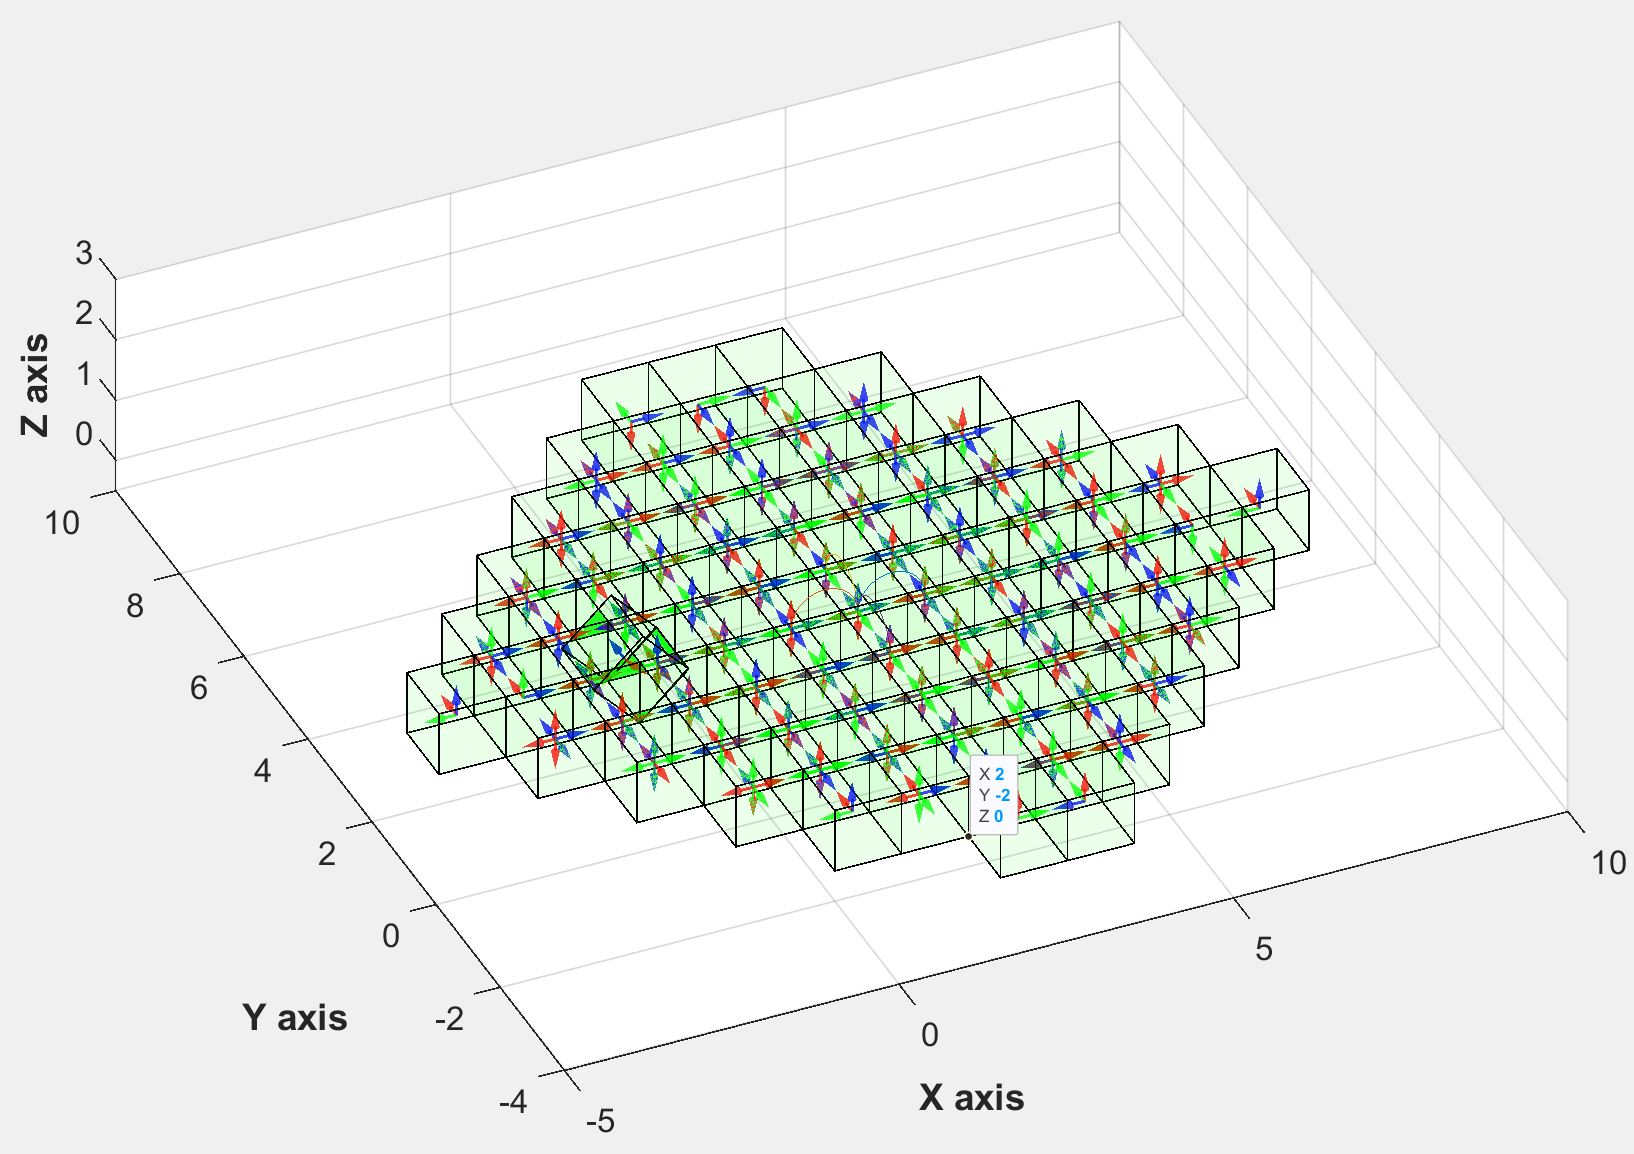
\includegraphics[width=0.5\textwidth]{image/cubeIteration2.jpg}
%    \includegraphics[page=2,width=.5\textwidth]{image/test2.pdf}	
	\label{fig:Cube2Case1}
	}
\caption{Initial configuration and the $6^{th}\ level$ of the cube's expansion} 
\end{figure}
\end{center}

\noindent Figure \ref{fig:twoCubePaths} shows that the two closed-paths are found at the same time after executing the proposed path planning algorithm six iterations. The initial configuration includes the position at $[2.5,2.5,0.5]$ and the orientation with three arrows $(green,red,blue)$ corresponding to $(Ox,Oy,-Oz)$ while the goal configuration has the same position with the initial position and the orientation with $(green,red,blue)$ corresponding to $(Ox,-Oy,Oz)$. If the initial or the goal configuration change their orientation, the algorithm will implement at different times and generates different paths.

\begin{center}
\begin{figure}[H]
\subfigure[The first closed-path of cube rolling]{
	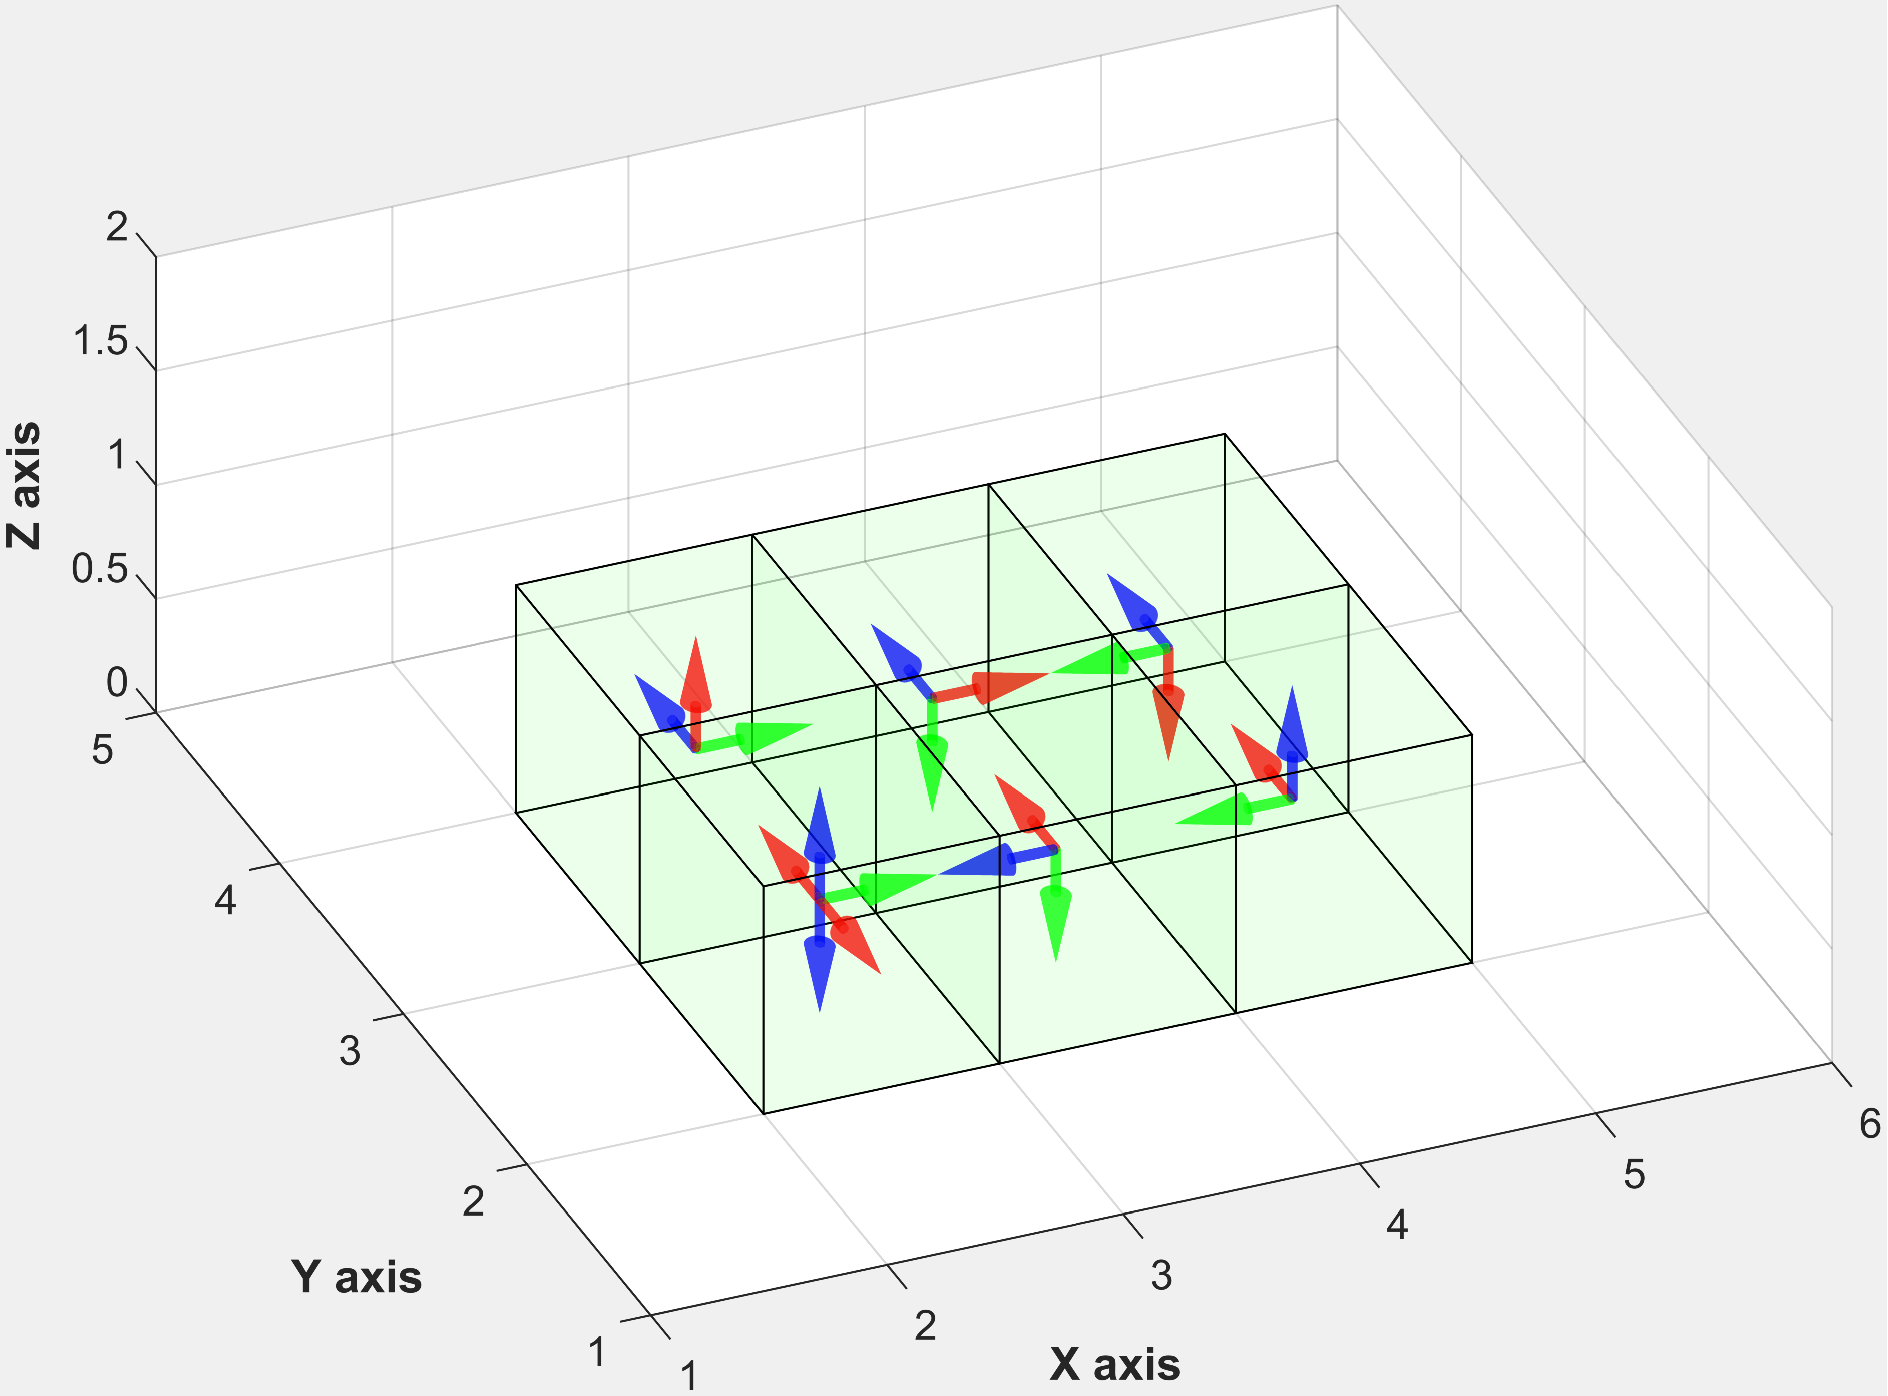
\includegraphics[width=0.5\textwidth]{image/cubePath0.pdf}
	\label{fig:cubePath1}
	}
\hfill
%\subfigure[First four paths of the cube rolling]{	
%	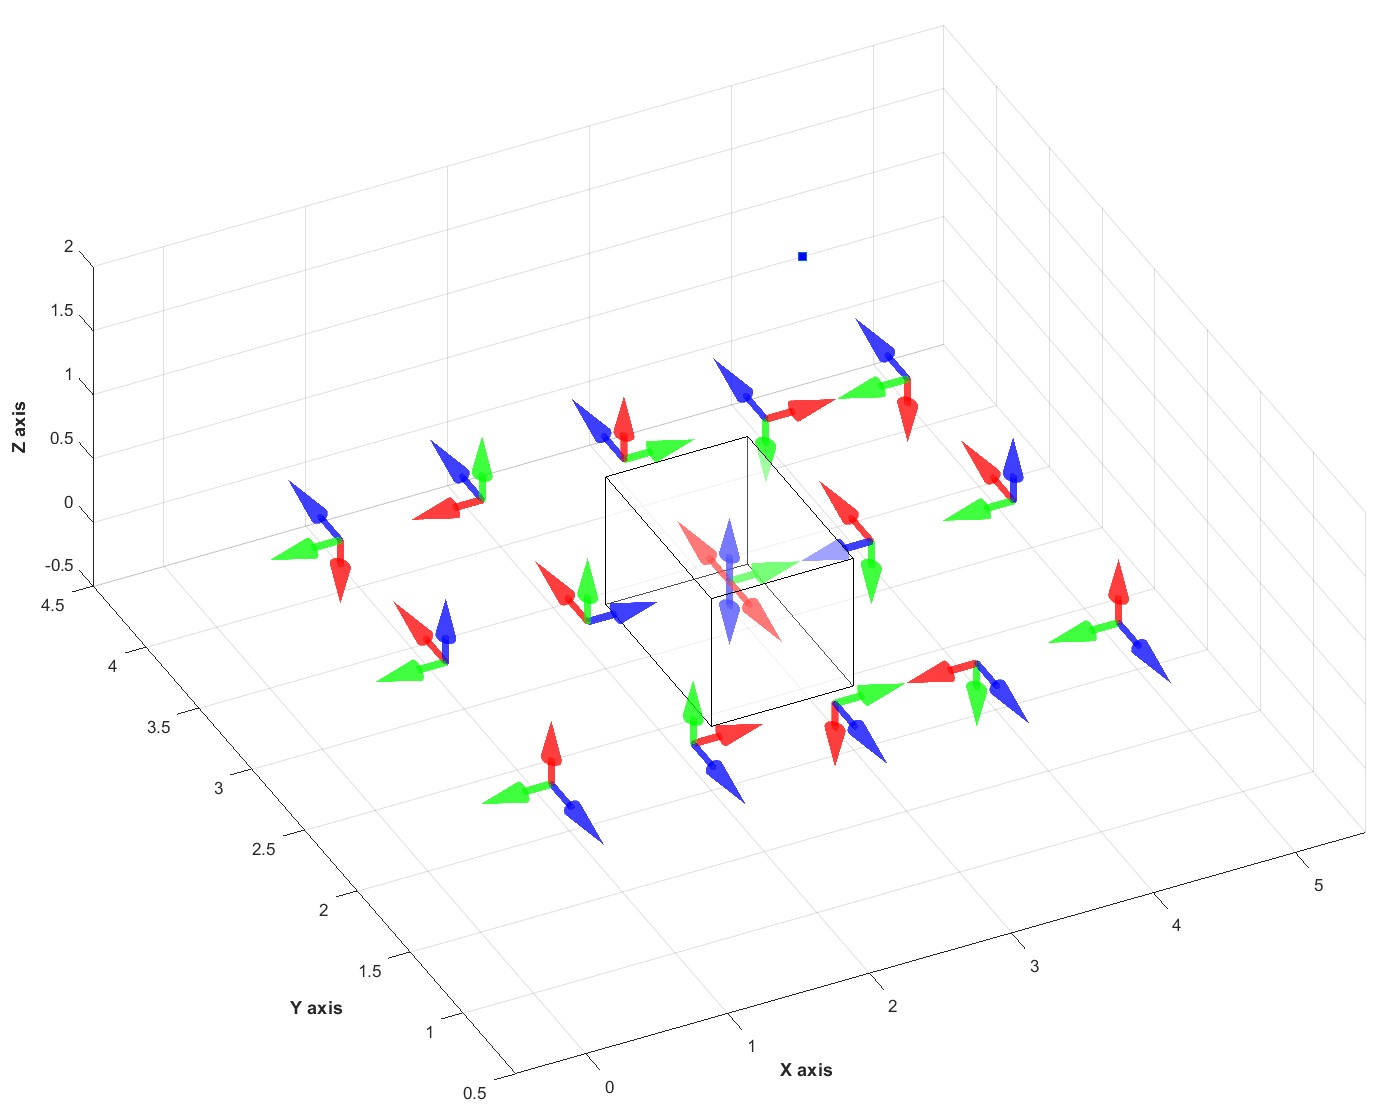
\includegraphics[width=0.5\textwidth]{image/cubePath4Dirs.jpg}
\subfigure[The second closed-path of cube rolling]{
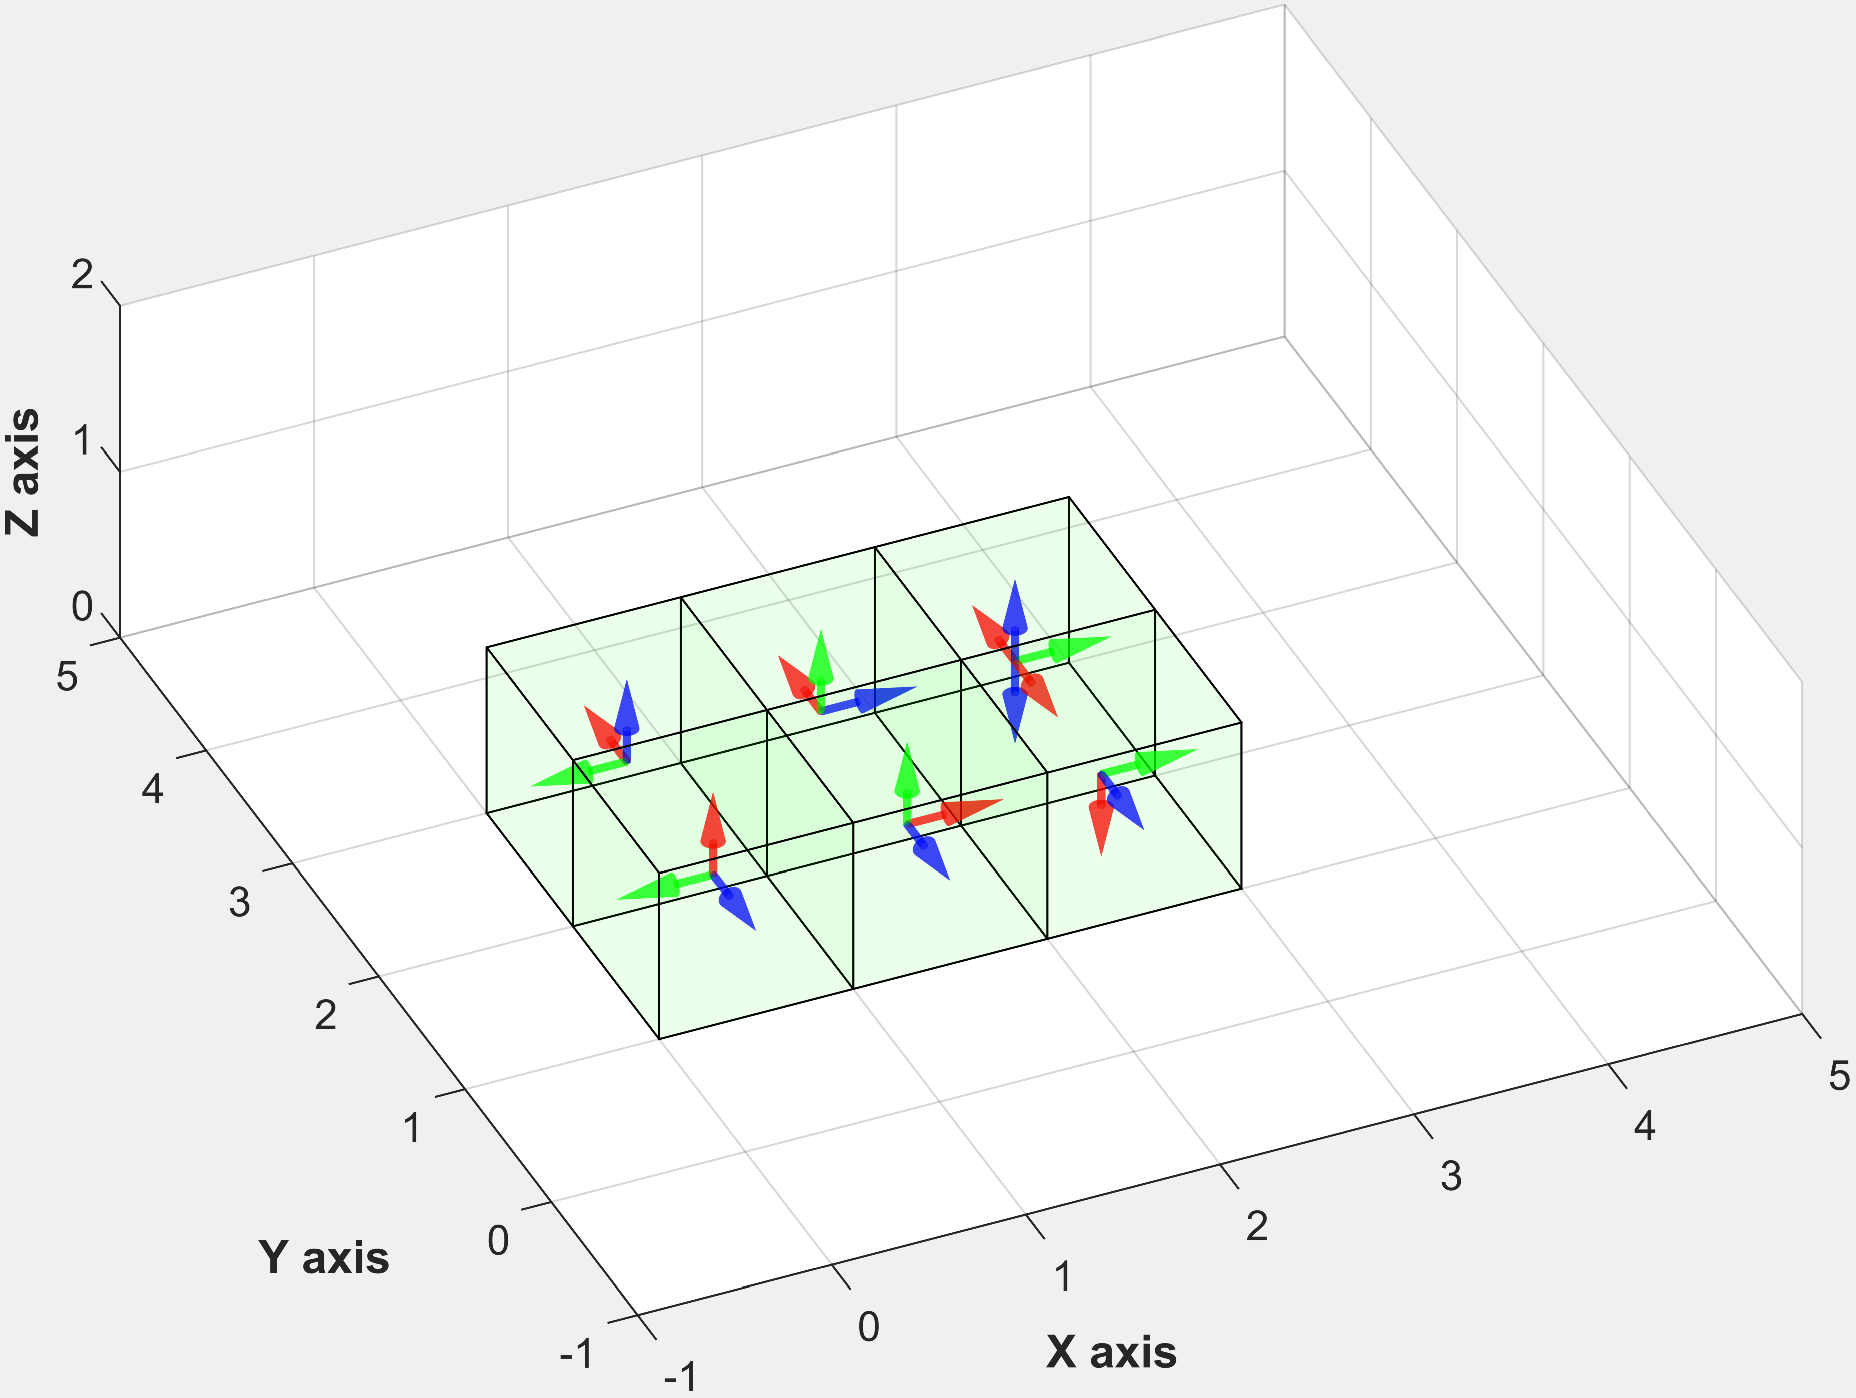
\includegraphics[width=0.5\textwidth]{image/cubePath2.pdf}
%    \includegraphics[page=2,width=.5\textwidth]{image/test2.pdf}	
	\label{fig:cubePath2}
	}
\caption{The two closed-path of cube rolling with initial and goal position at $[2.5,2.5,0.5]$}
\label{fig:twoCubePaths}
\end{figure}
\end{center}


%%\noindent\uline{Result}: 
%\begin{figure}[h]
%\centering
%	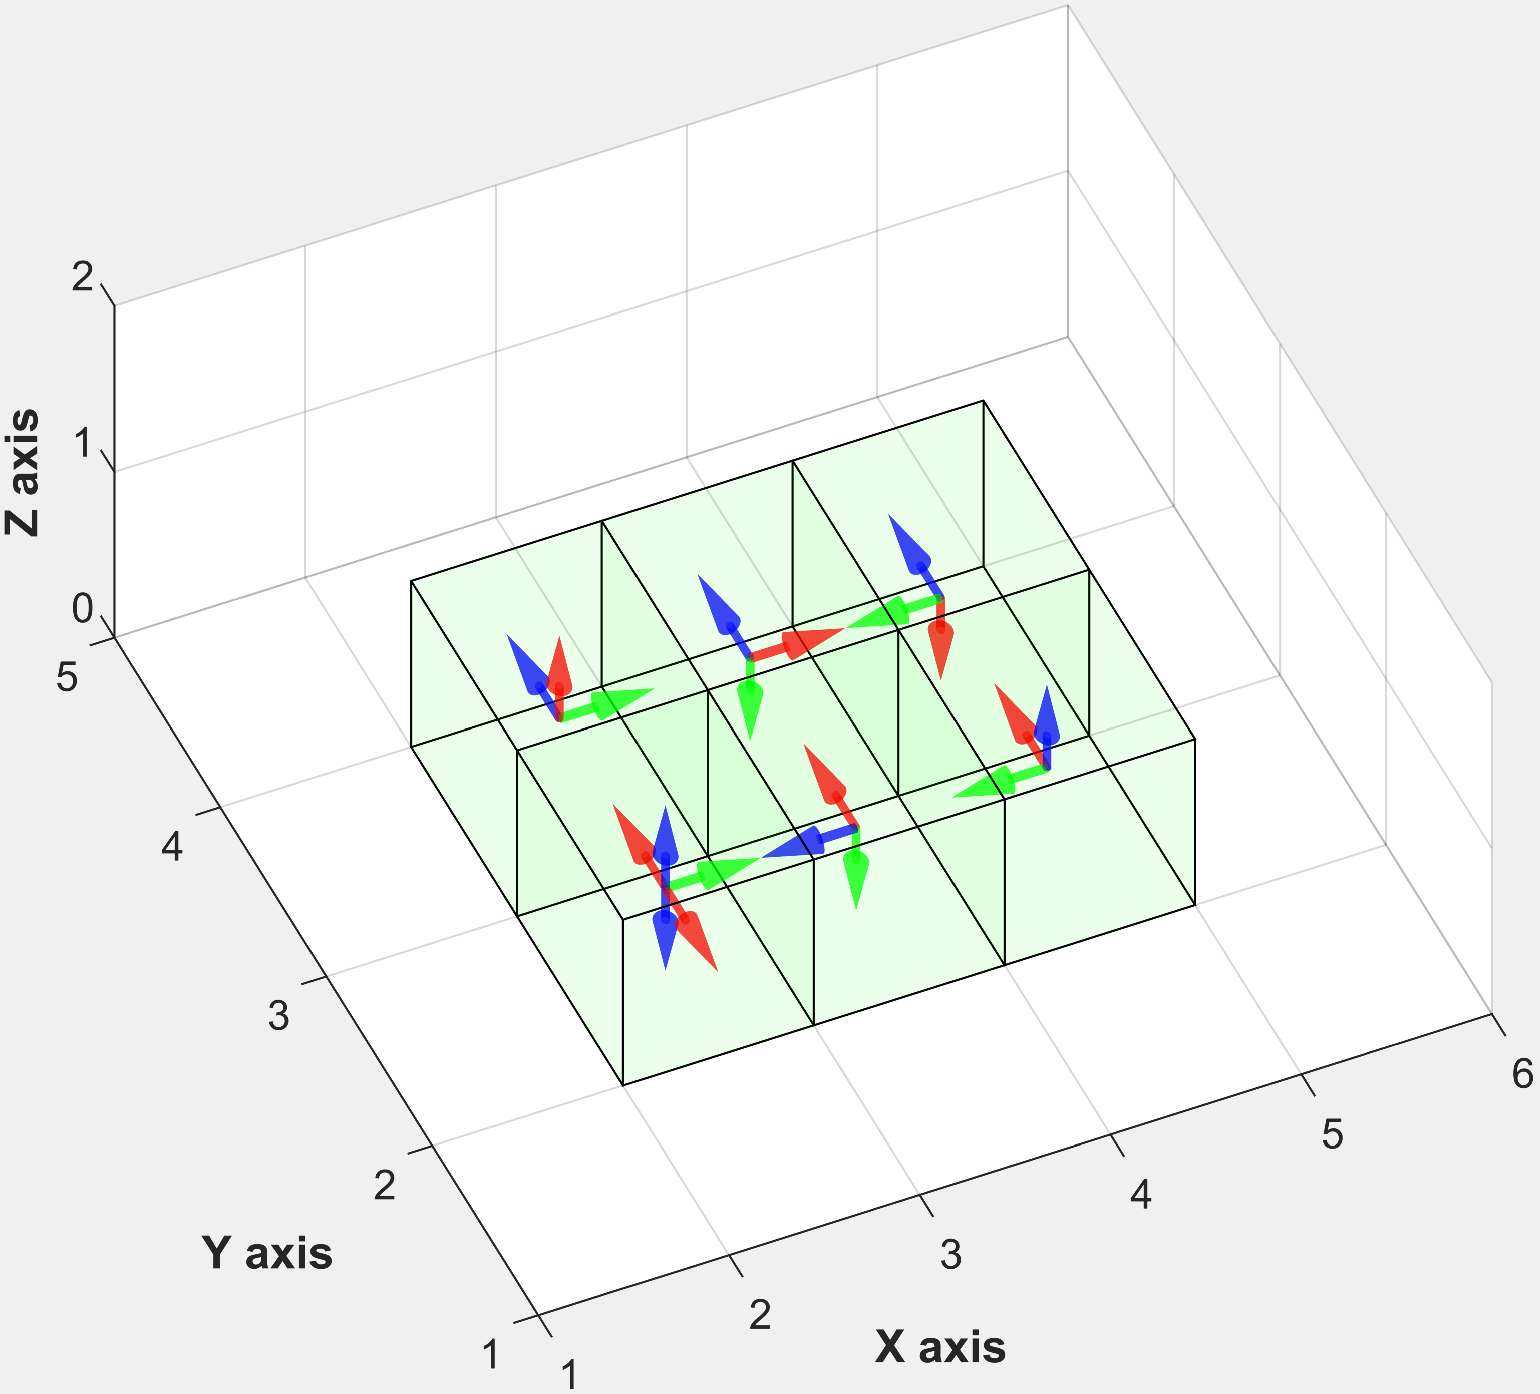
\includegraphics[width=0.5\textwidth]{image/cubePath1.pdf}
%%	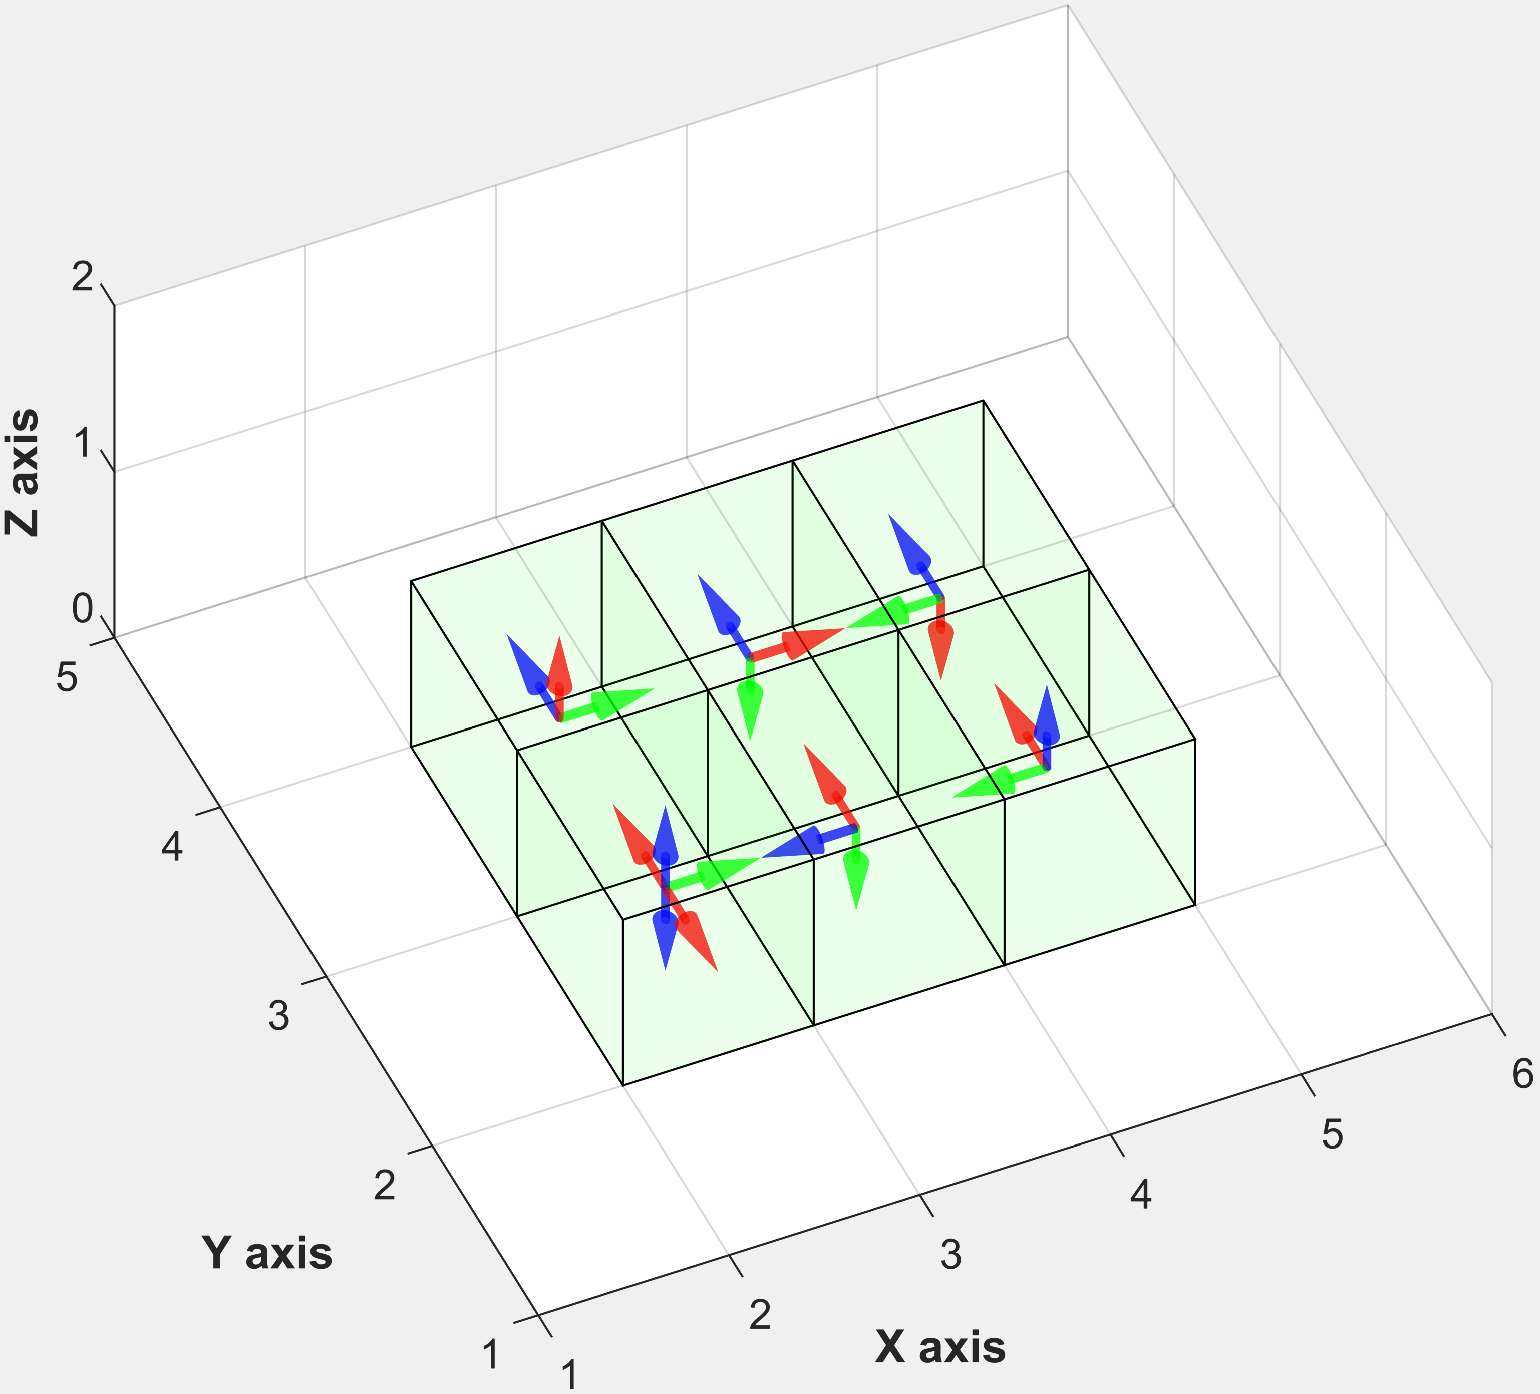
\includepdf[pages=-,pagecommand={},width=0.5\textwidth]{image/cubePath1.pdf}
%	\caption{Shortest path of cube rolling}
%	\label{fig:cubePath1}
%\end{figure}

%\begin{figure}[h]
%	\centering
%		\begin{subfigure}[t]
%			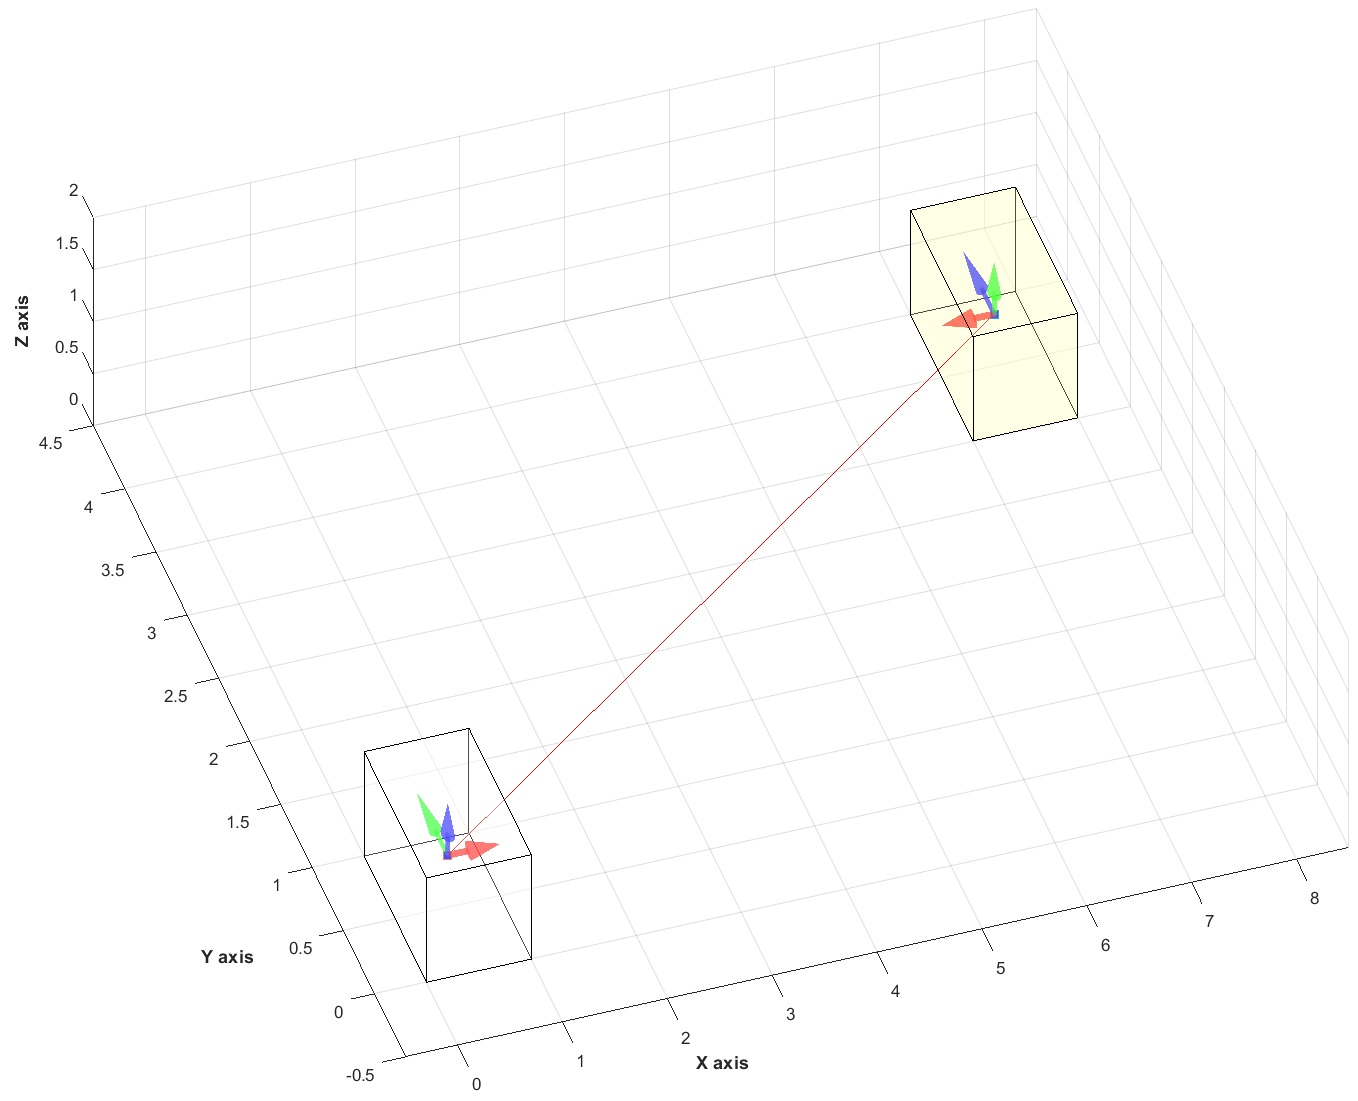
\includegraphics[width=0.5\textwidth]{image/cubePathCase2Initial.jpg}
%			\subcaption{Long distance between two configurations}
%			\label{fig:Cube1Case2}
%		\end{subfigure}
%%\hfill
%		\begin{subfigure}[t]
%			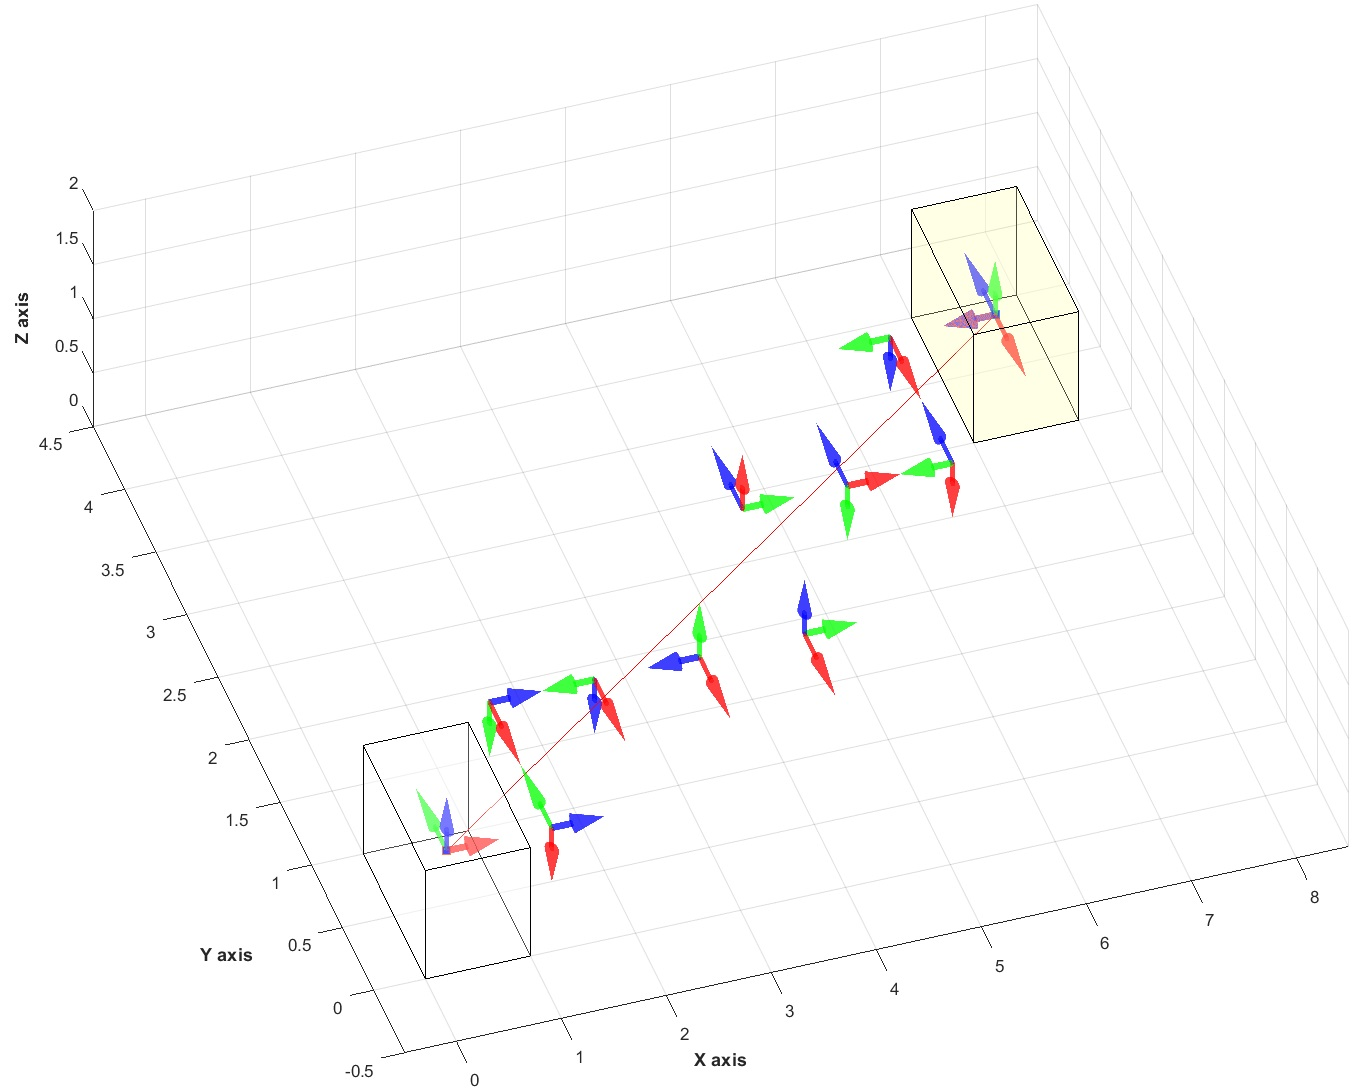
\includegraphics[width=0.5\textwidth]{image/cubePathCase2DirecRolling.jpg}
%			\subcaption{Directly rolling from initial configuration to goal configuration}
%			\label{fig:Cube2Case2}
%		\end{subfigure}
%\end{figure}

%%
%%
%%
%\clearpage
%\newpage
%\noindent Although considering the case study within \\ 

%\noindent \uline{Extension case}: The proposed algorithm in this study can be applied for the case study of long distance between the initial and goal configurations. 
%Figure \ref{fig:cubeLongDist} shows an example with two different paths.
%Shortest path-finding algorithm is added to the original algorithm to find the shortest path from start point to the goal point. 
%After finishing this step, the cube updated to a new orientation with different orientation at the goal configuration. Then, the original algorithm will be implemented from the updated cube to the goal configuration.
%Assume that the initial configuration is at $S_1$ and the goal configuration is at $S2$. In the first step, the red line segment $S_1S_2$ shows the shortest distance from start position to goal position. The cube will roll through this line segment and achieve the updated orientation at the goal position called shortest path for the case of long distance. 
%
%%\begin{center}
%\begin{figure}[H]
%\centering
%\subfigure[Path1]{
%	\includegraphics[width=0.75\textwidth]{image/cubeCase2Path1.jpg}
%	\label{fig:cubeLongDistPath1}
%	}
%\hfill
%\subfigure[Path2]{
%	\includegraphics[width=0.75\textwidth]{image/cubeCase2Path2.jpg}
%	\label{fig:cubeLongDistPath2}
%	}
%\caption{The case study of long distance between the initial and goal configurations}
%\label{fig:cubeLongDist}
%\end{figure}
%%\end{center}
%%
%%
%%
%%
%%==================================================================================
%%                               Tetrahedron solid
%%==================================================================================
%%
%%
%%
\clearpage
\newpage
\subsection{Tetrahedron solid}
\noindent\uline{Properties} 
As can be seen from Figure \ref{fig:tetraGeo1}, the Tetrahedron has constructed by four faces of the equilateral triangles. Then the height of triangle $ABC$ is $AM$ and $AM=DM=a\sqrt{3}/2$.
Because of $r=OH=a\sqrt{6}/12$ (the radius of insphere) and $R=OA=a\sqrt{6}/4$ (the radius of circumsphere), the height of tetrahedron is $AH=OA+OH=a\sqrt{6}/3$. The rotation angle is $\beta$ determined by supplementary angles $\alpha=\arctan(2\sqrt{2})$ or $\beta=\pi-\alpha = \pi-\arctan(2\sqrt{2})$.
 
\begin{figure}[h]
\centering
	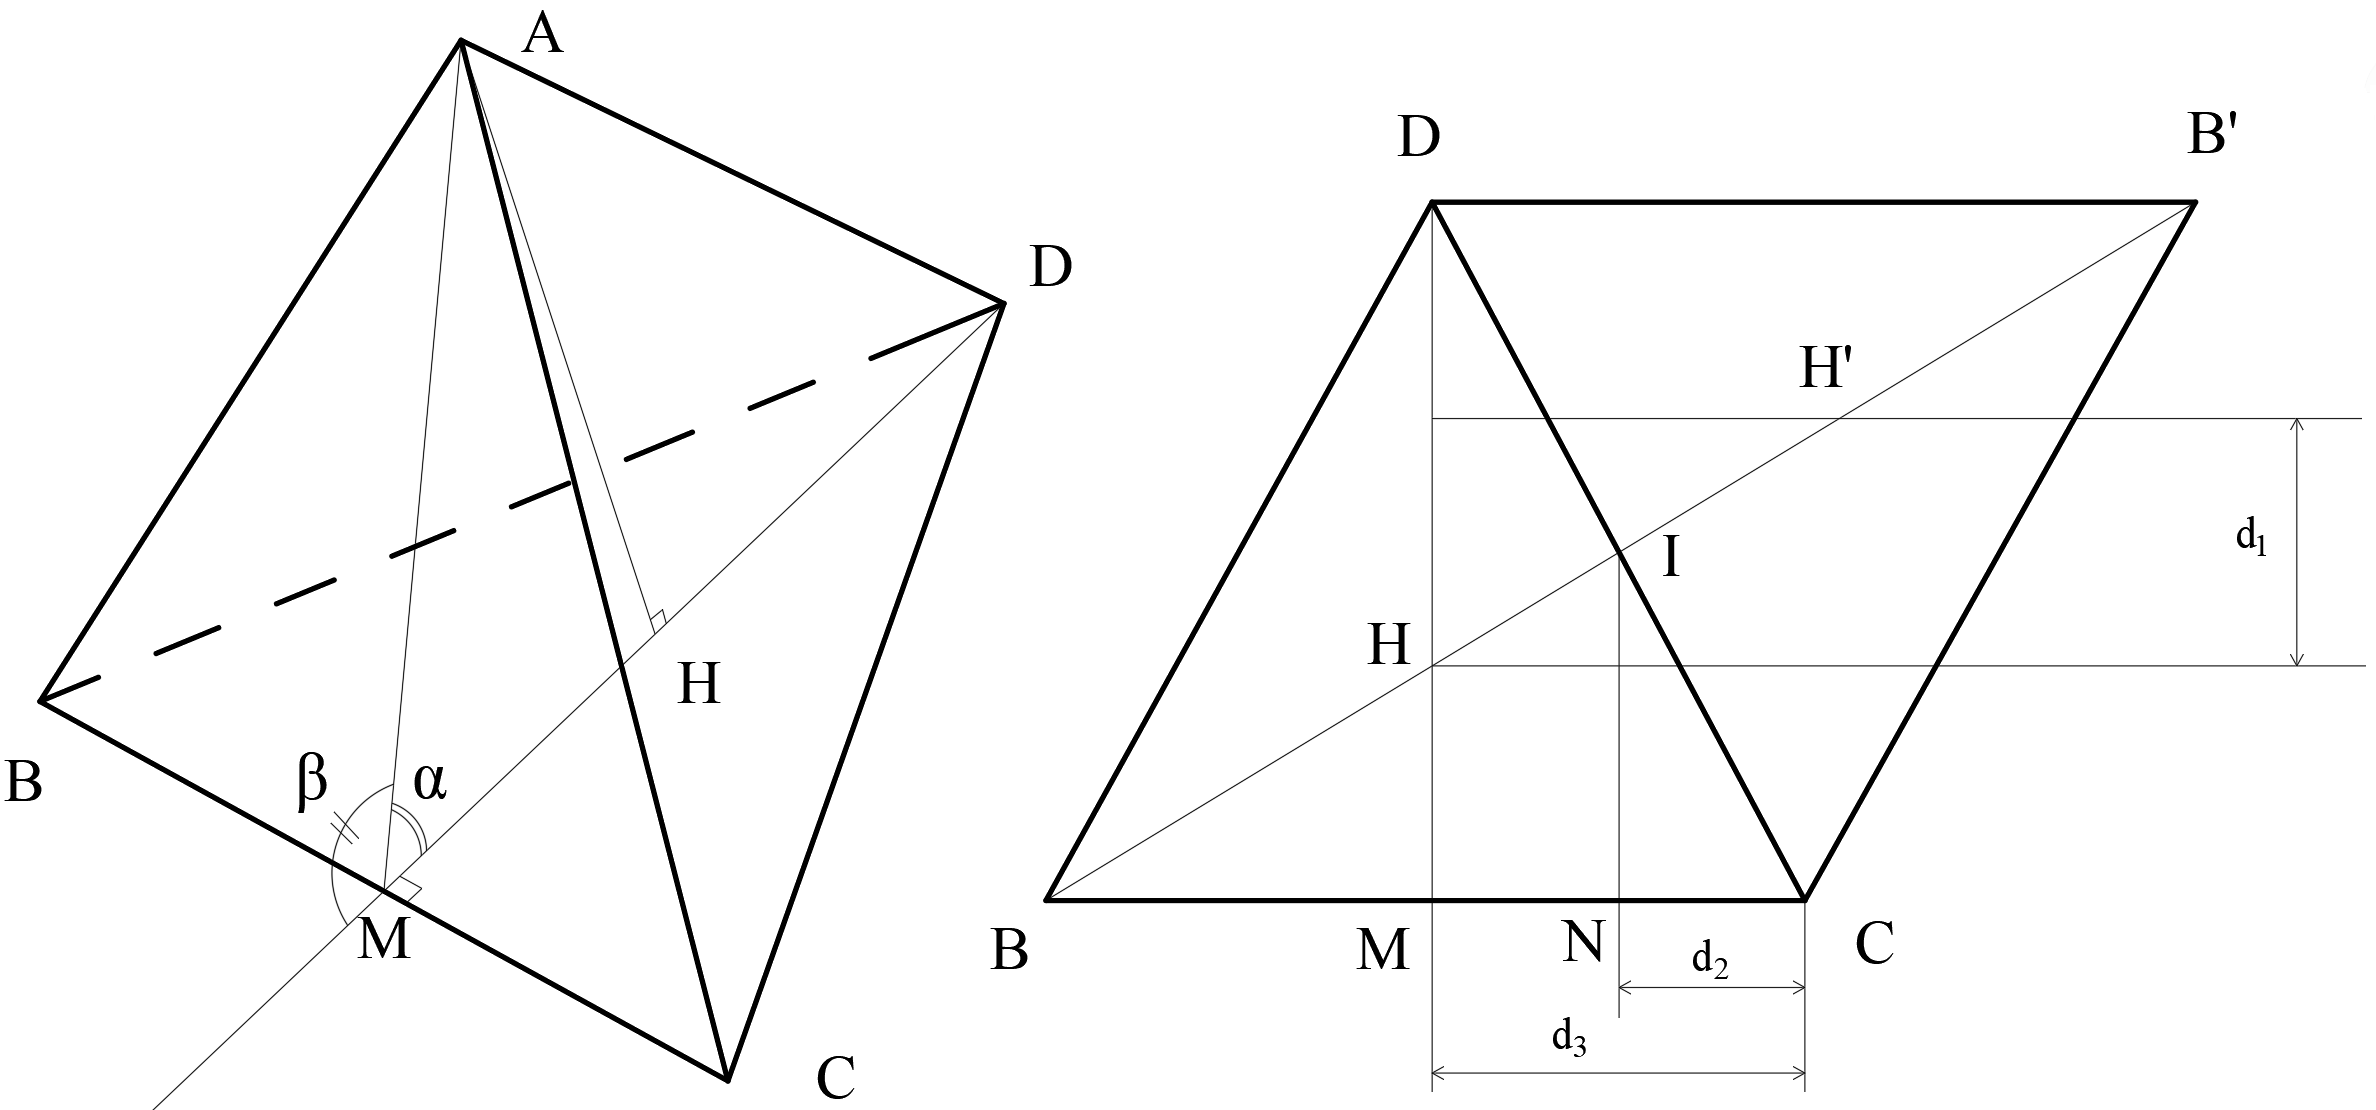
\includegraphics[width=\textwidth]{image/TetraGeo11.png}
%	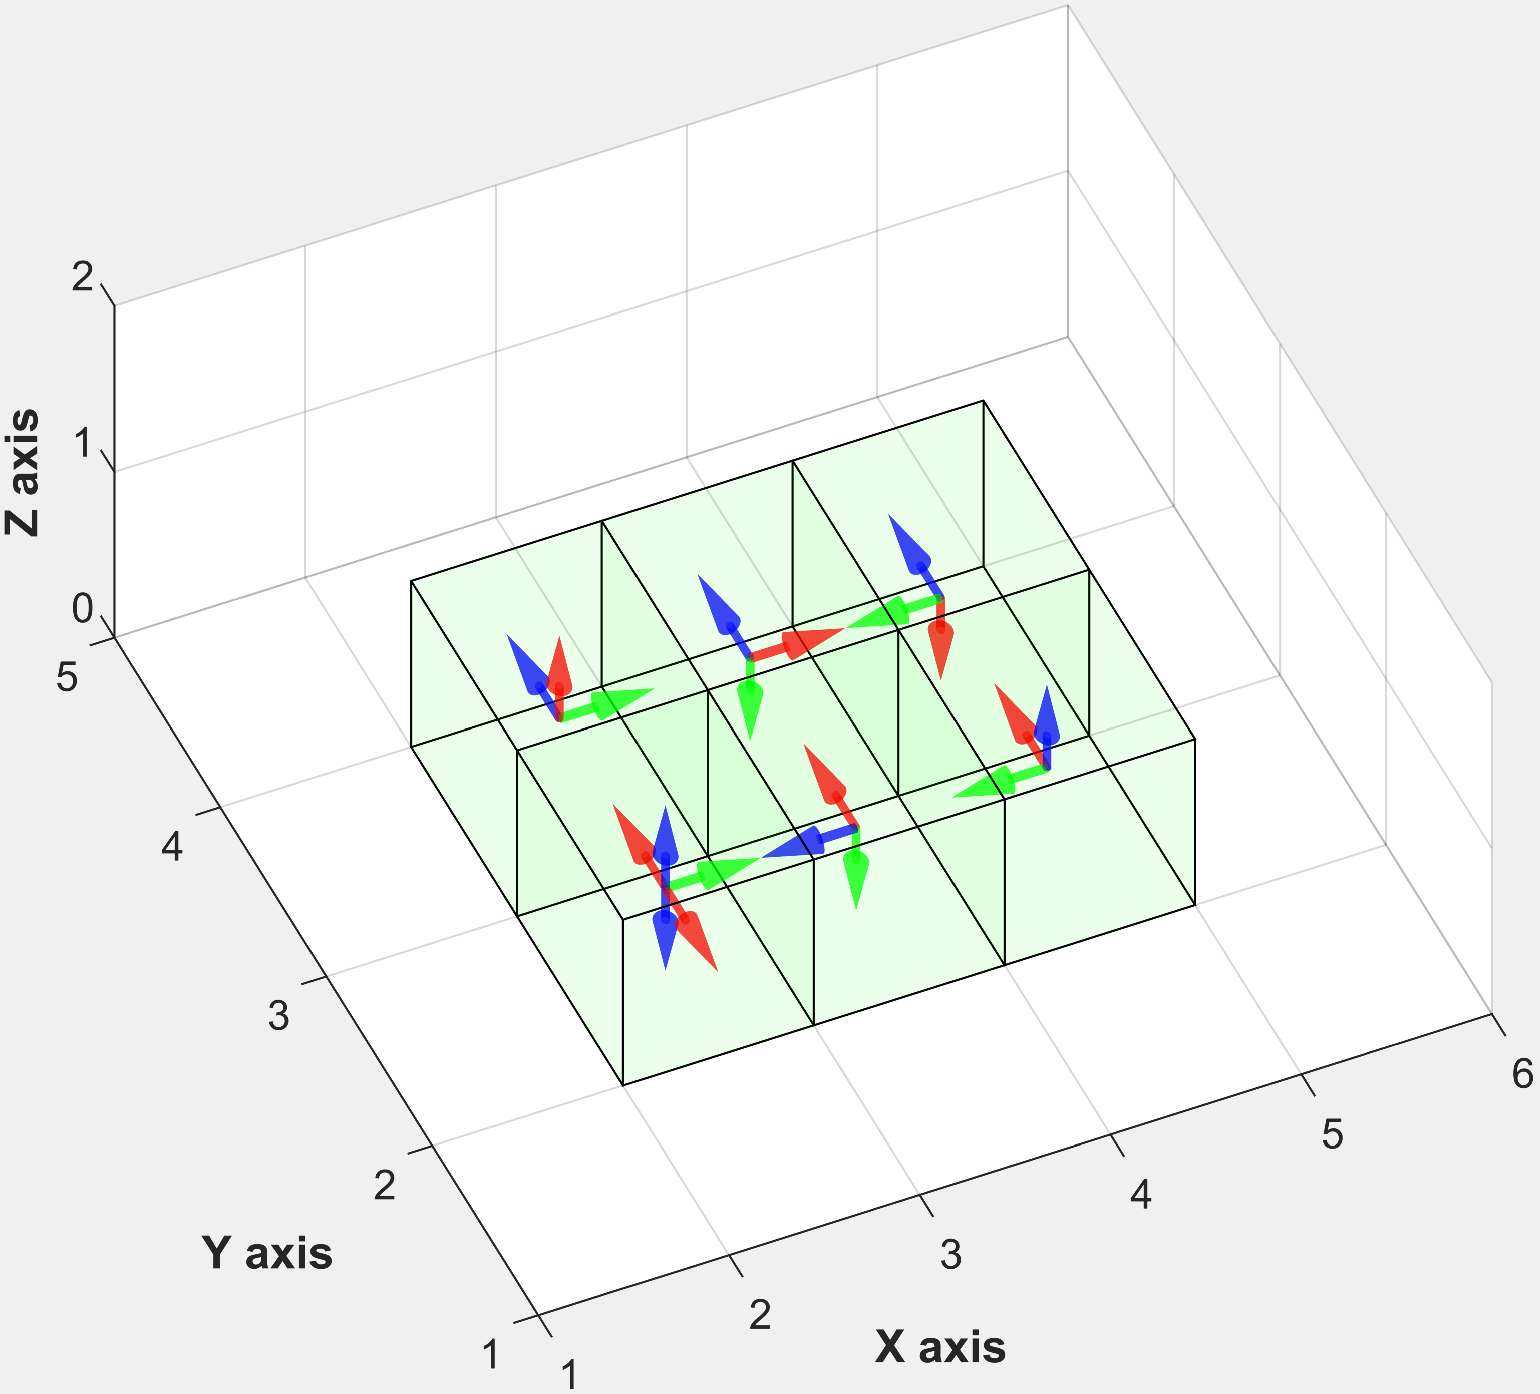
\includepdf[pages=-,pagecommand={},width=0.5\textwidth]{image/cubePath1.pdf}
	\caption{Tetrahedron geometrical properties}
	\label{fig:tetraGeo1}
\end{figure}

\noindent\uline{Path Planning}:
The case study of the tetrahedron in this study is the same as the rolling cube path-finding which only considering the path planning through rolling from initial configuration to origin coordinate with different orientations. 
Figure \ref{fig:TetraPathFiding} illustrates two of four cases of the tetrahedron path-finding within rolling (red and cyan arrows are pointing down to plane respectively). 
A tetrahedron has symmetry properties with indistinguishable for any two faces, edges and vertices. To be more specific, dihedral triangles have the same three angles within $\ang{60}$. 
In one cycle of rolling a tetrahedron around any vertices, the tetrahedron always achieves the initial configuration due to six times of rolling ($6*\ang{60}=\ang{360}$, a full circle). \\

\begin{center}
\begin{figure}[h]
\subfigure[Tetrahedron path 1]{
	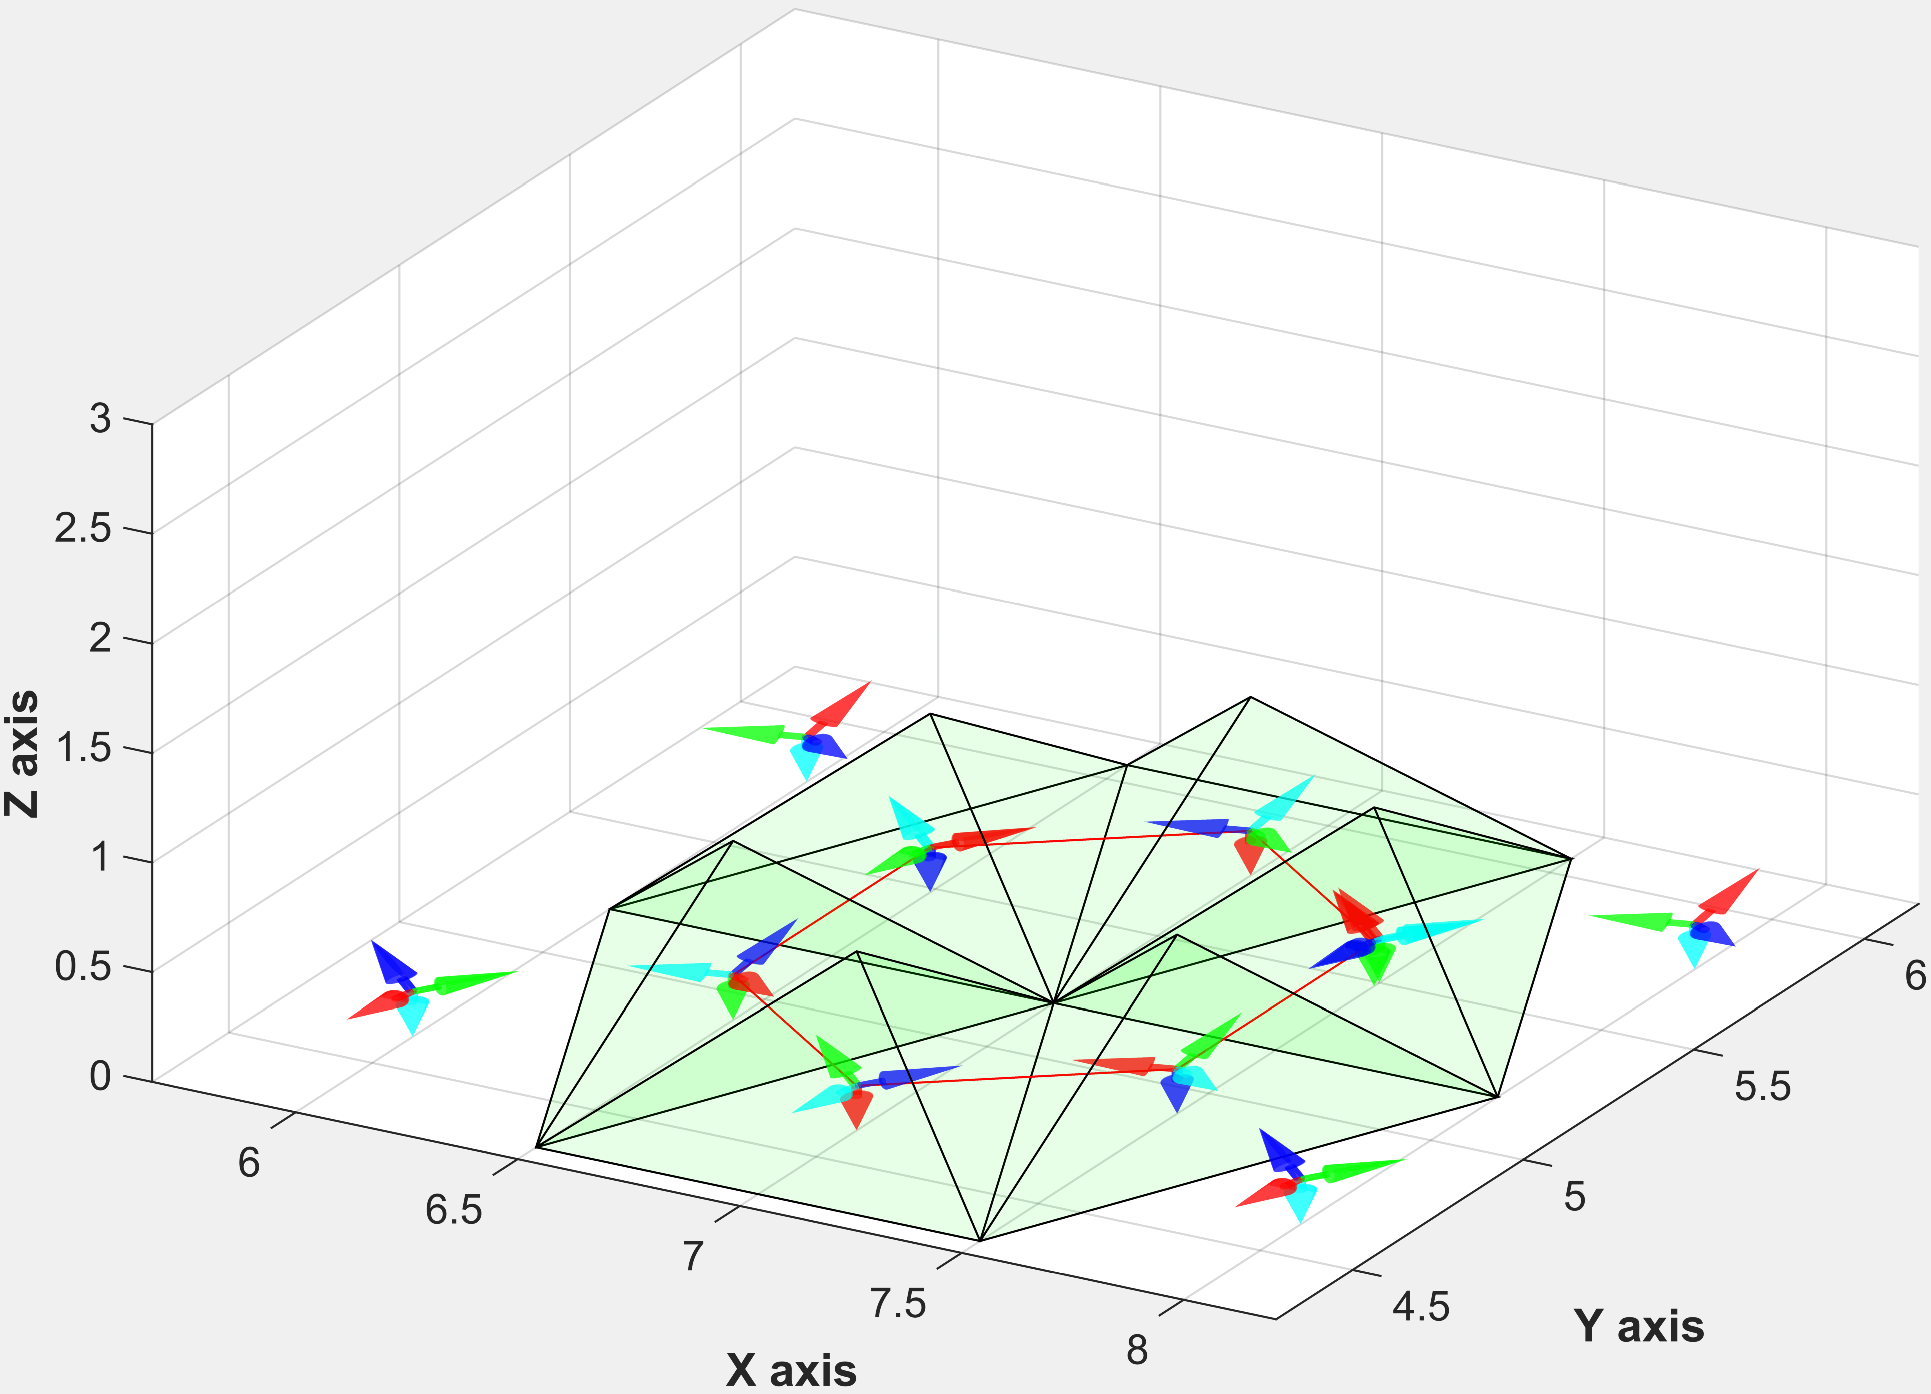
\includegraphics[width=0.5\textwidth]{image/tetraPath2.pdf}
	\label{fig:Tetra1Case1}
	}
\hfill
\subfigure[Tetrahedron path 2]{
	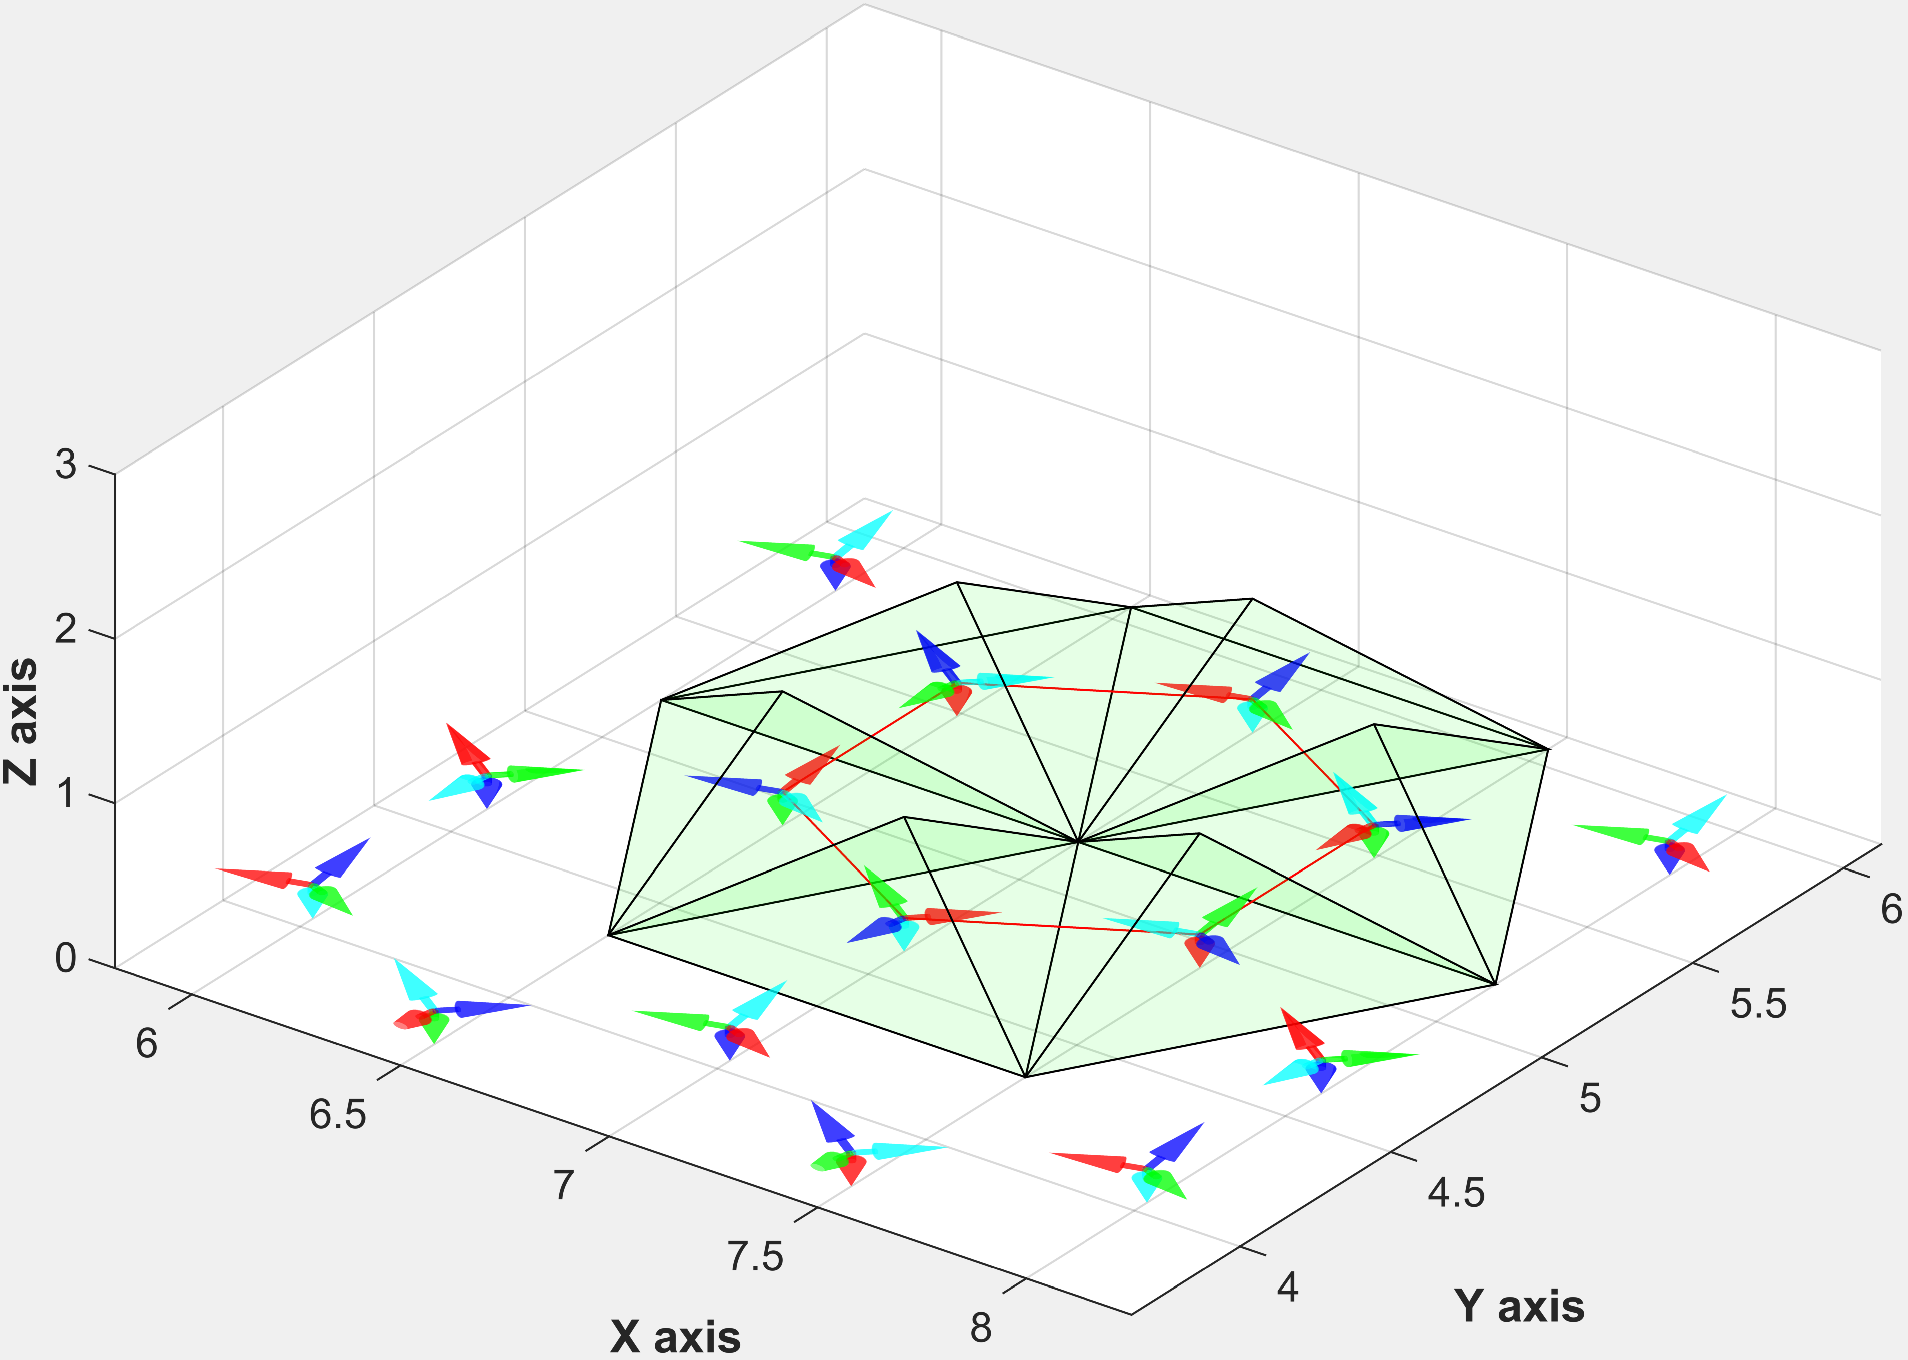
\includegraphics[width=0.5\textwidth]{image/tetraPath1.pdf}
	\label{fig:Tetra2Case1}
	}
\caption{The two of four cases}
\label{fig:TetraPathFiding}
\end{figure}
\end{center}
%%
%%
%%
%%==================================================================================
%%                              Octahedron solid
%%==================================================================================
%%
%%
%%
\clearpage
\newpage
\subsection{Octahedron solid}
\noindent\uline{Properties}: 
An octahedron has six vertices and twelve edges which generates eight equilateral triangles. Figure \ref{fig:octaGeo1} shows that an octahedron has length $a$ with the based surface $ABC$. In each step of a rolling, the octahedron will roll into three direction through edge contacts with same rotation angle which is determined as below.   

\begin{figure}[h]
\centering
	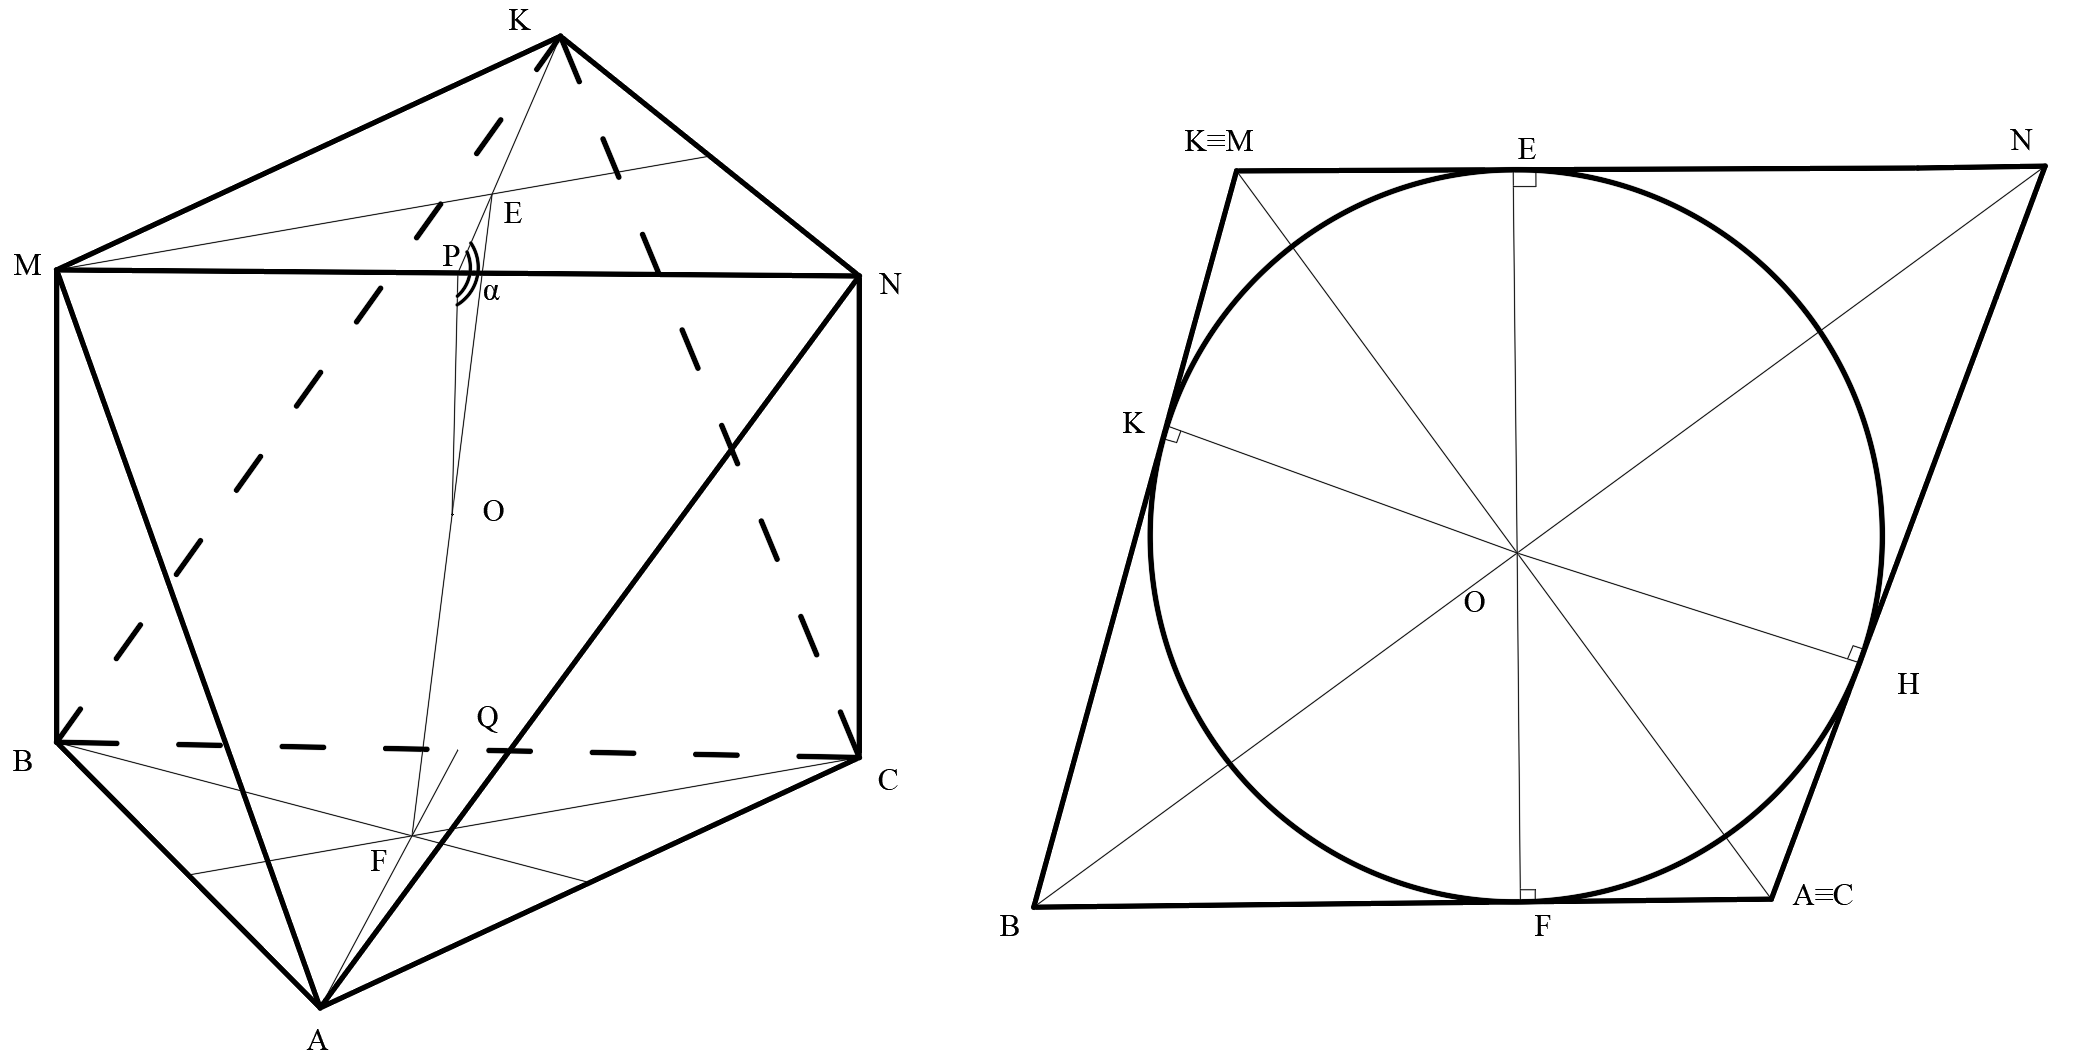
\includegraphics[width=\textwidth]{image/octaGeo11.png}
%	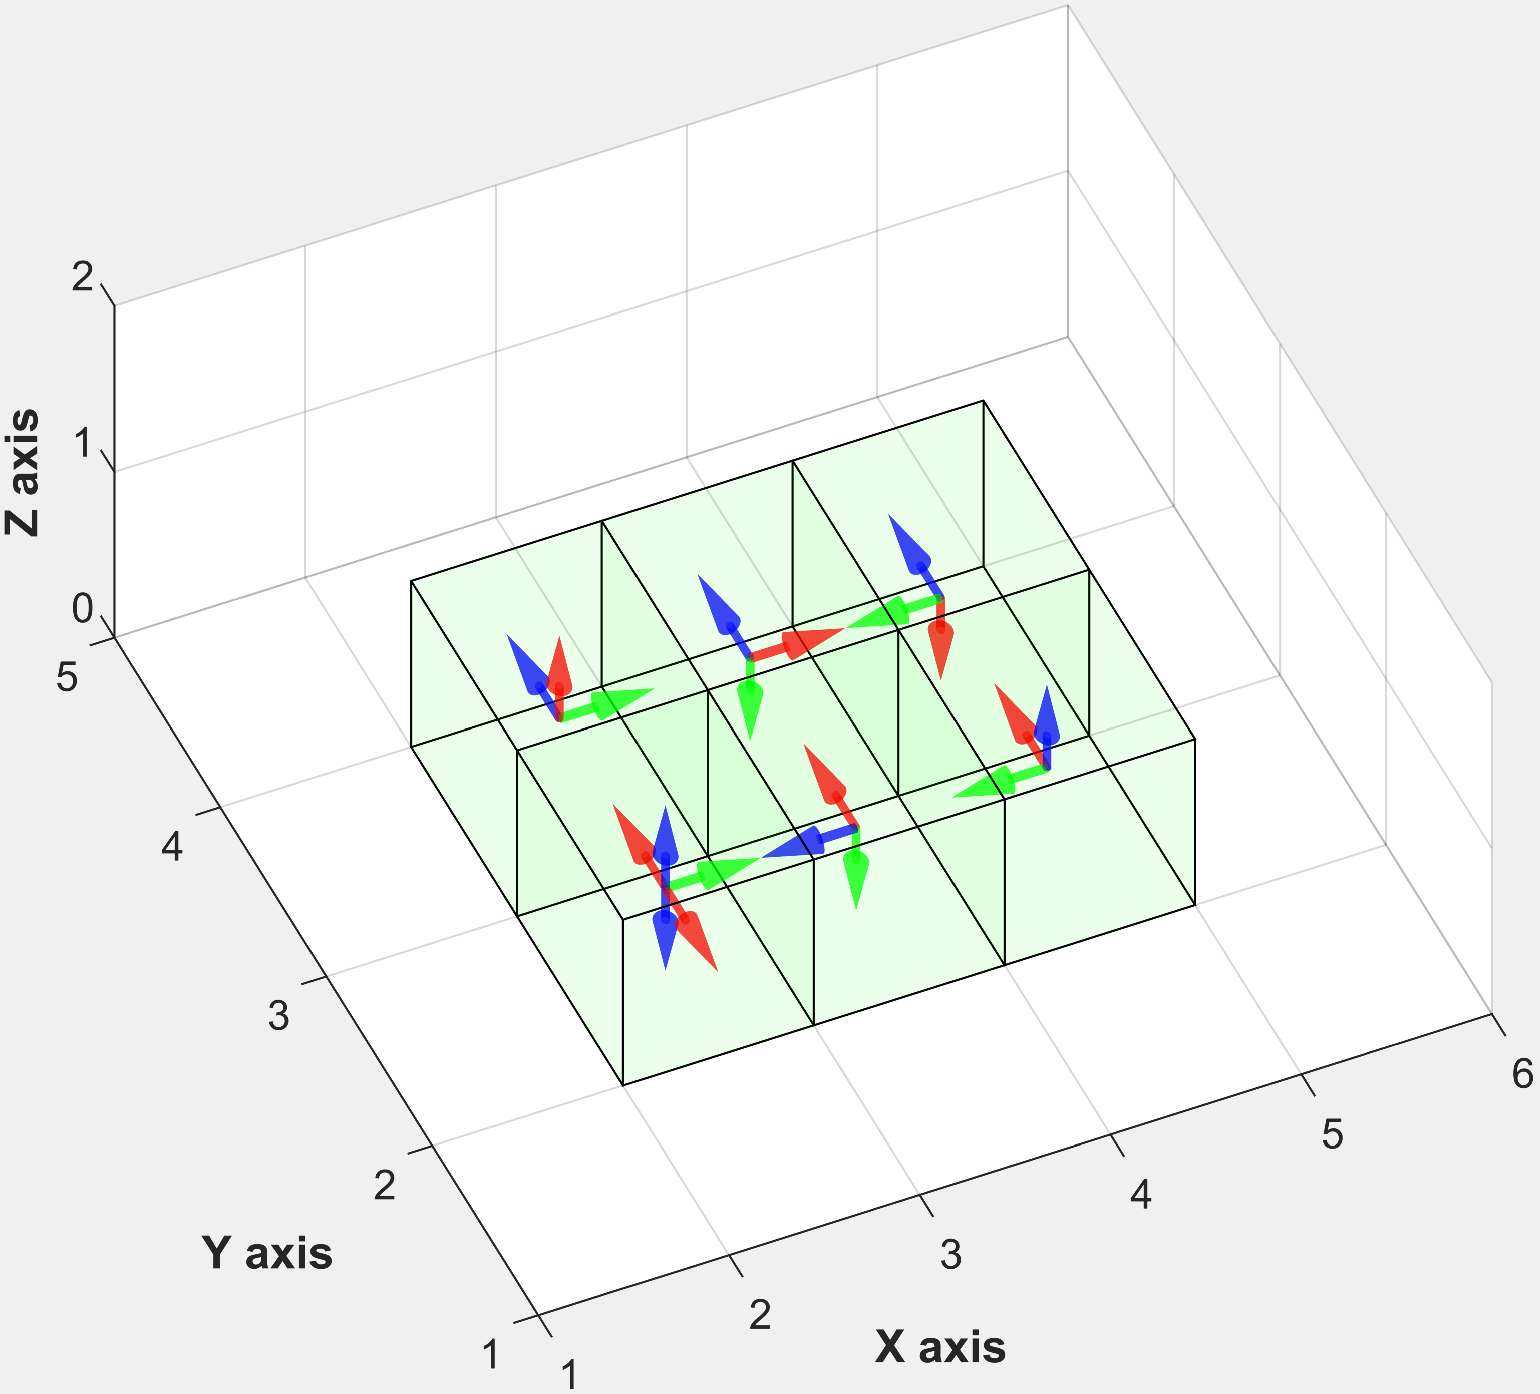
\includepdf[pages=-,pagecommand={},width=0.5\textwidth]{image/cubePath1.pdf}
	\caption{Octahedron geometrical properties}
	\label{fig:octaGeo1}
\end{figure}


%\begin{wrapfigure}{H}{0.25\textwidth} %this figure will be at the right
%    \centering
%    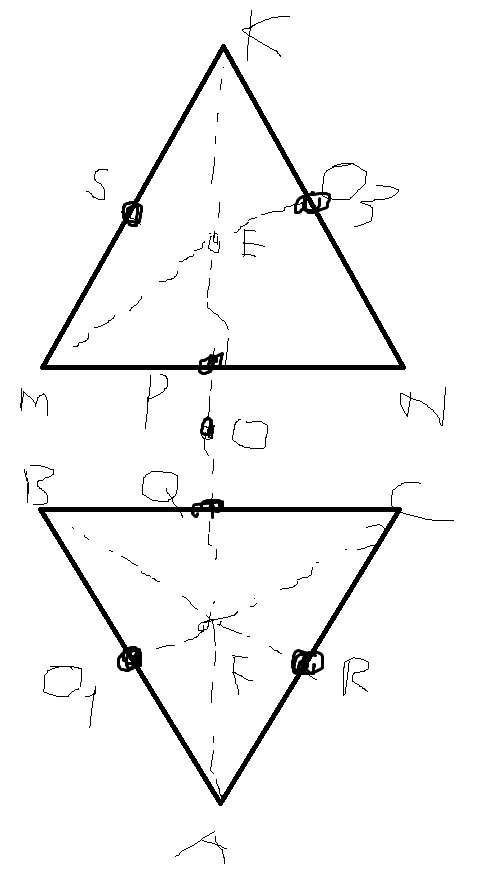
\includegraphics[width=0.25\textwidth]{image/octaGeo2.png}
%\end{wrapfigure}

\noindent From Figure \ref{fig:octaGeo1} we have:

\begin{equation*} 
\label{octa:eq0}
\begin{split}
AK & = 2OK = 2\sqrt{(MK^2-MO^2)} = a\sqrt{2}\\
\Rightarrow OK & = OM = ON = a\frac{\sqrt{2}}{2}\\
\end{split}
\end{equation*}

\noindent To find the rotation angle, the supplementary angle should be calculated first. 

\begin{equation*} 
\label{octa:eq2}
\begin{split}
\alpha & = \angle OPK = \arctan{\frac{OK}{OP}} = \arctan{\sqrt{2}}
\end{split}
\end{equation*}

\noindent Then, the rotation angle has the result as  $\beta = \pi-2\alpha = \pi-2\arctan{\sqrt{2}}$, \\

\noindent Due to $\angle POK=\ang{90}$, a distance from the center $O$ of the octahedron to the center of bottom triangle is calculated.

\begin{equation*} 
\label{octa:eq3}
\begin{split}
\frac{1}{OE^2} & = \frac{1}{OP^2}+\frac{1}{OK^2}\\
			   & = \frac{1}{(\frac{\sqrt{2}}{2})^2}+\frac{1}{(\frac{1}{2})^2}\\
\Rightarrow OE & = \frac{\sqrt{6}}{6}
\end{split}
\end{equation*}

\noindent Applying the theory of the equilateral triangle

\begin{equation*} 
\label{octa:eq4}
\begin{split}
EO & = OF = a\frac{\sqrt{6}}{6}\\
KE & = FA = a\frac{\sqrt{3}}{3}\\
EP & = FQ = a\frac{\sqrt{3}}{6}
\end{split}
\end{equation*}

\noindent\uline{Path planning}:
Based on the classical path planning which is the movement from point to other points, the octahedron path planning within rolling has three directions to move. In the Figure \ref{fig:octaGeo1}, the bottom layer $\triangle ABC$ which contacts to $OXY$ can roll with the directions $FQ, FO_1, FR$. The distance between two shortest positions is $2FR= 2a\frac{\sqrt{3}}{6}=a\frac{\sqrt{3}}{3}$. 

\noindent As can be seen from Figure \ref{fig:octaPath1}, the shortest path within red line includes ten line segments for rolling the octahedron. The total length of the path equals $10a\frac{\sqrt{3}}{3}$ (edge length of the octahedron is $a$).

\begin{figure}[h!]
\subfigure[The first closed-path of Octahedron path rolling]{
	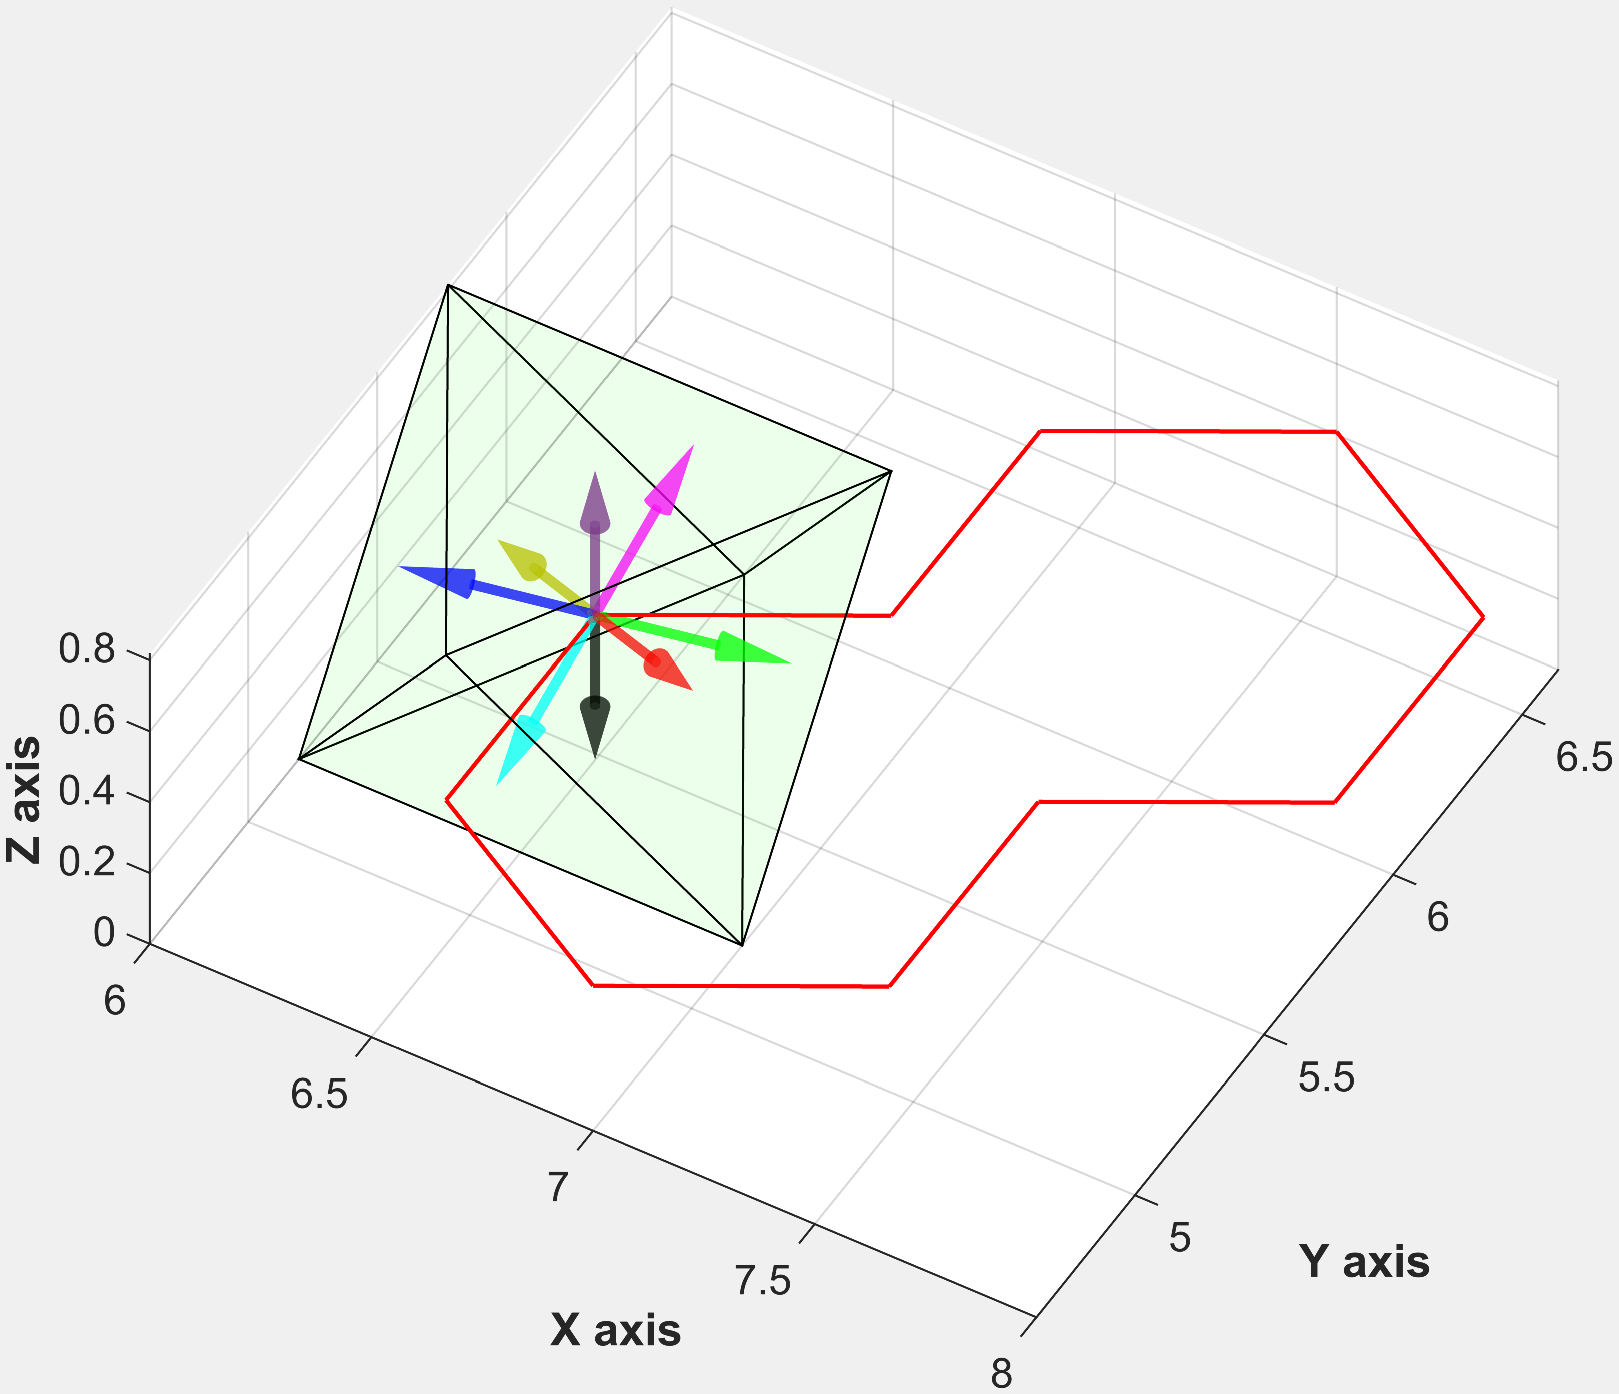
\includegraphics[width=0.5\textwidth]{image/octoPath1.pdf}
	\label{fig:octaPath1}
	}
\hfill
\subfigure[The second closed-path of Octahedron path rolling]{
	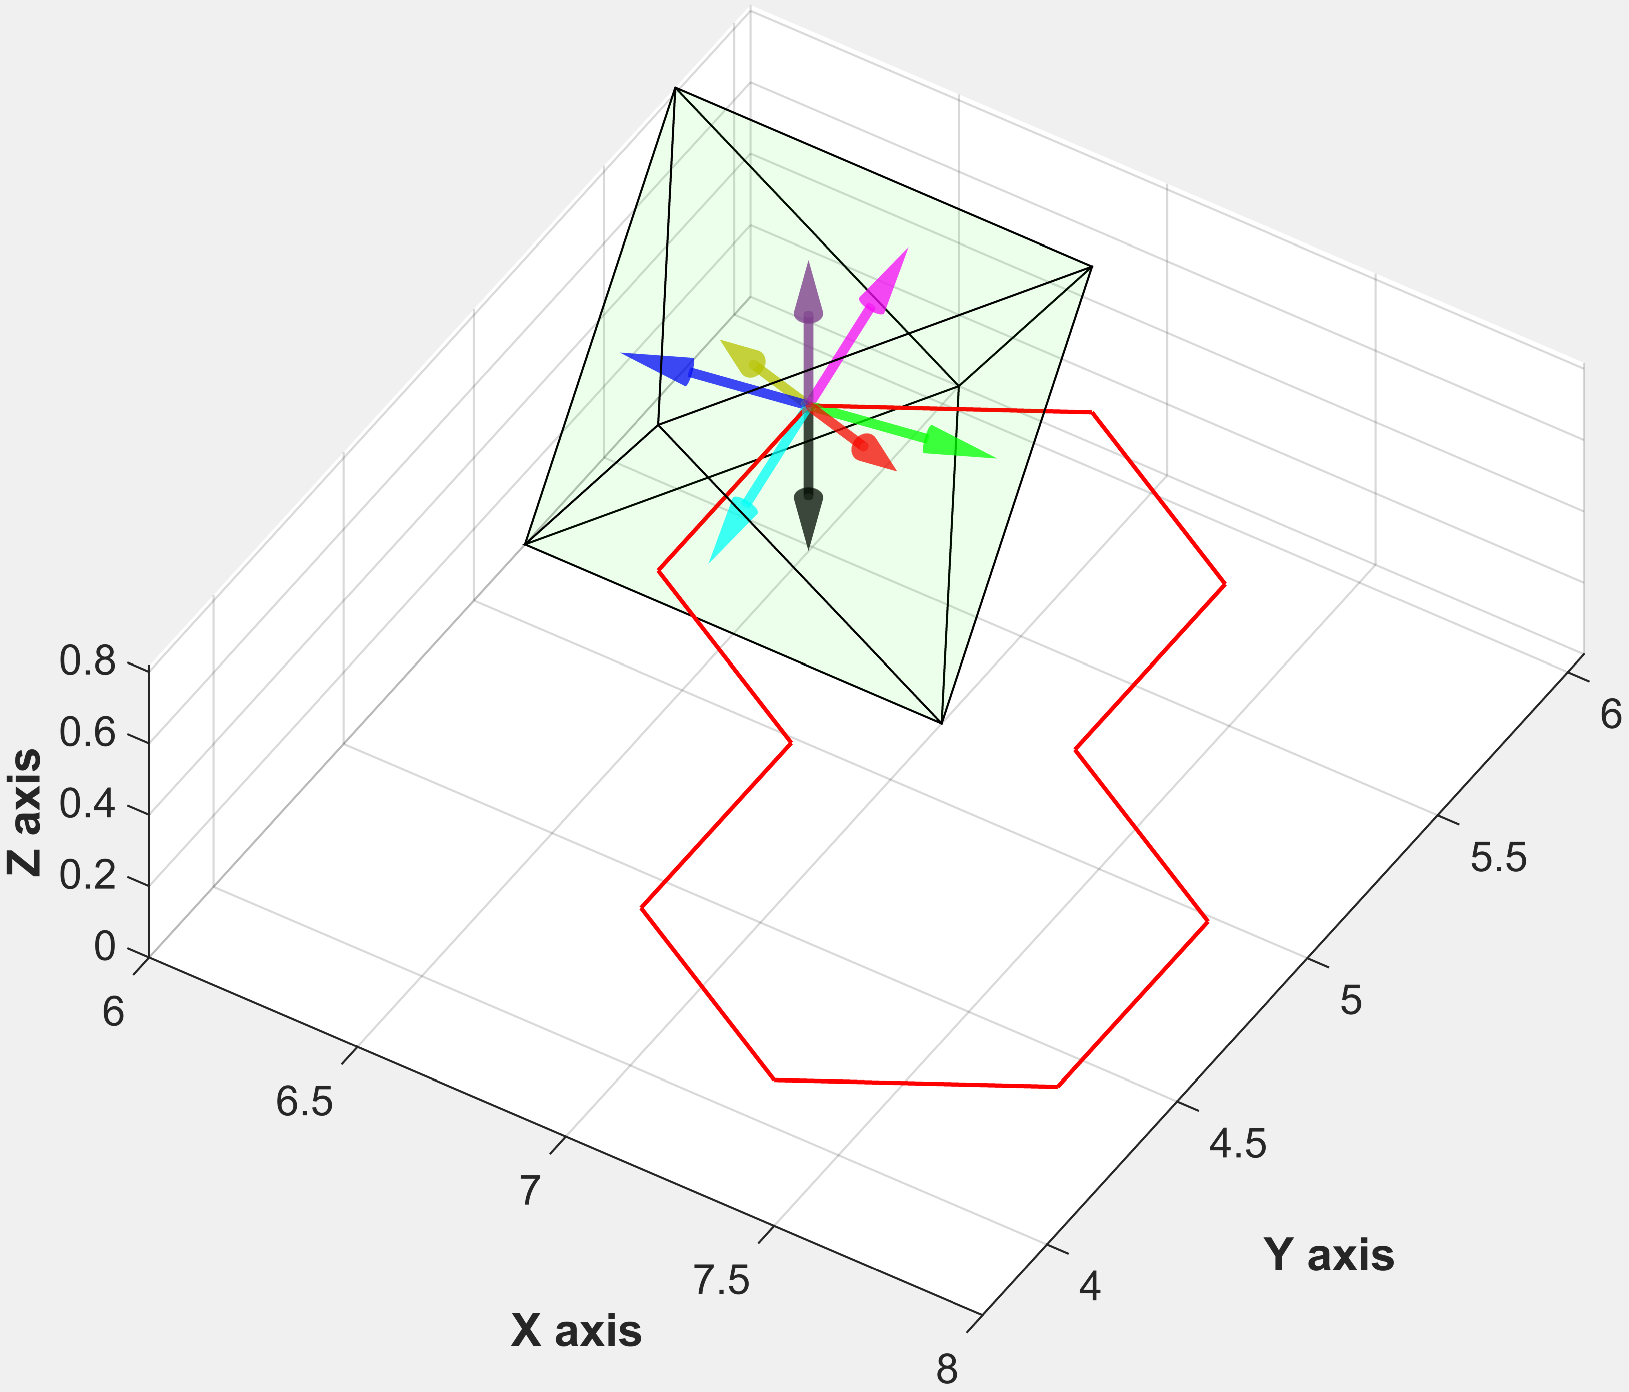
\includegraphics[width=0.5\textwidth]{image/octoPath2.pdf}
	\label{fig:octaPath2}
	}
\subfigure[The third closed-path of Octahedron path rolling]{
	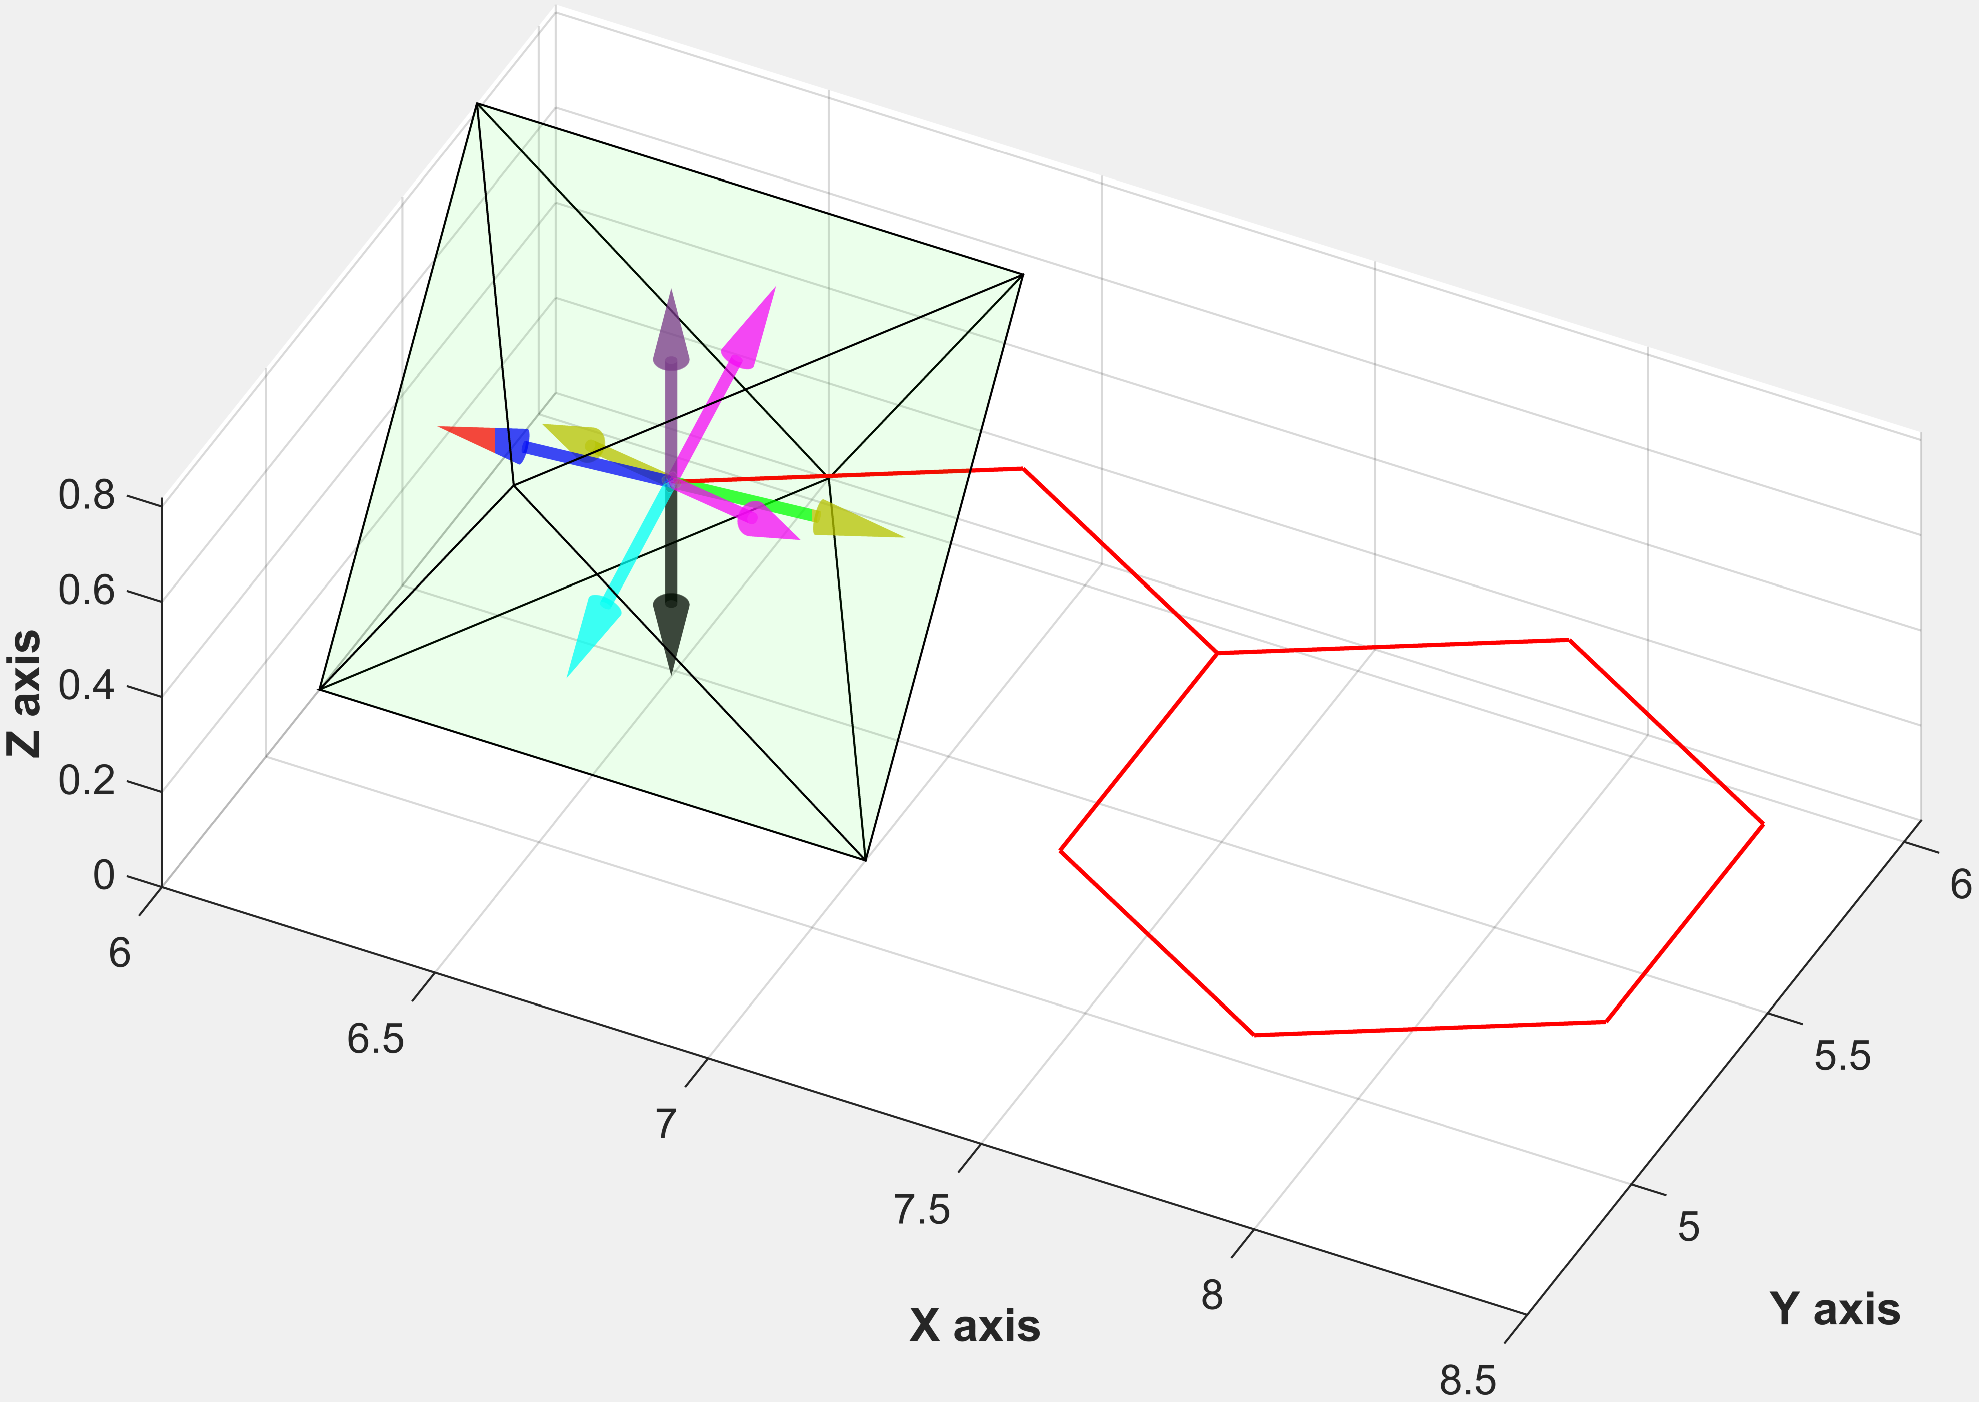
\includegraphics[width=0.5\textwidth]{image/octoPath3.pdf}
	\label{fig:octaPath3}
	}
\caption{Three shortest paths of octahedron based rolling}
\label{fig:octaPaths}
\end{figure}

%%
%%
%%==================================================================================
%%                       Icosahedron solid
%%==================================================================================
%%
%%
%%
\clearpage
\newpage
\subsection{Icosahedron solid}
\noindent\uline{Properties}:
The convex regular icosahedron in Figure \ref{fig:icosaGeo2} is one of the five regular Platonic solids has 12 vertices, 20 triangular faces, and 30 edges. 
Assume that the icosahedron has the edge length with $a$. 
The crossing surface of the solid at vertex $A$ perpendicular with $OD$ will generate a pentagon $ABCEF$.

\begin{figure}[h]
\centering
	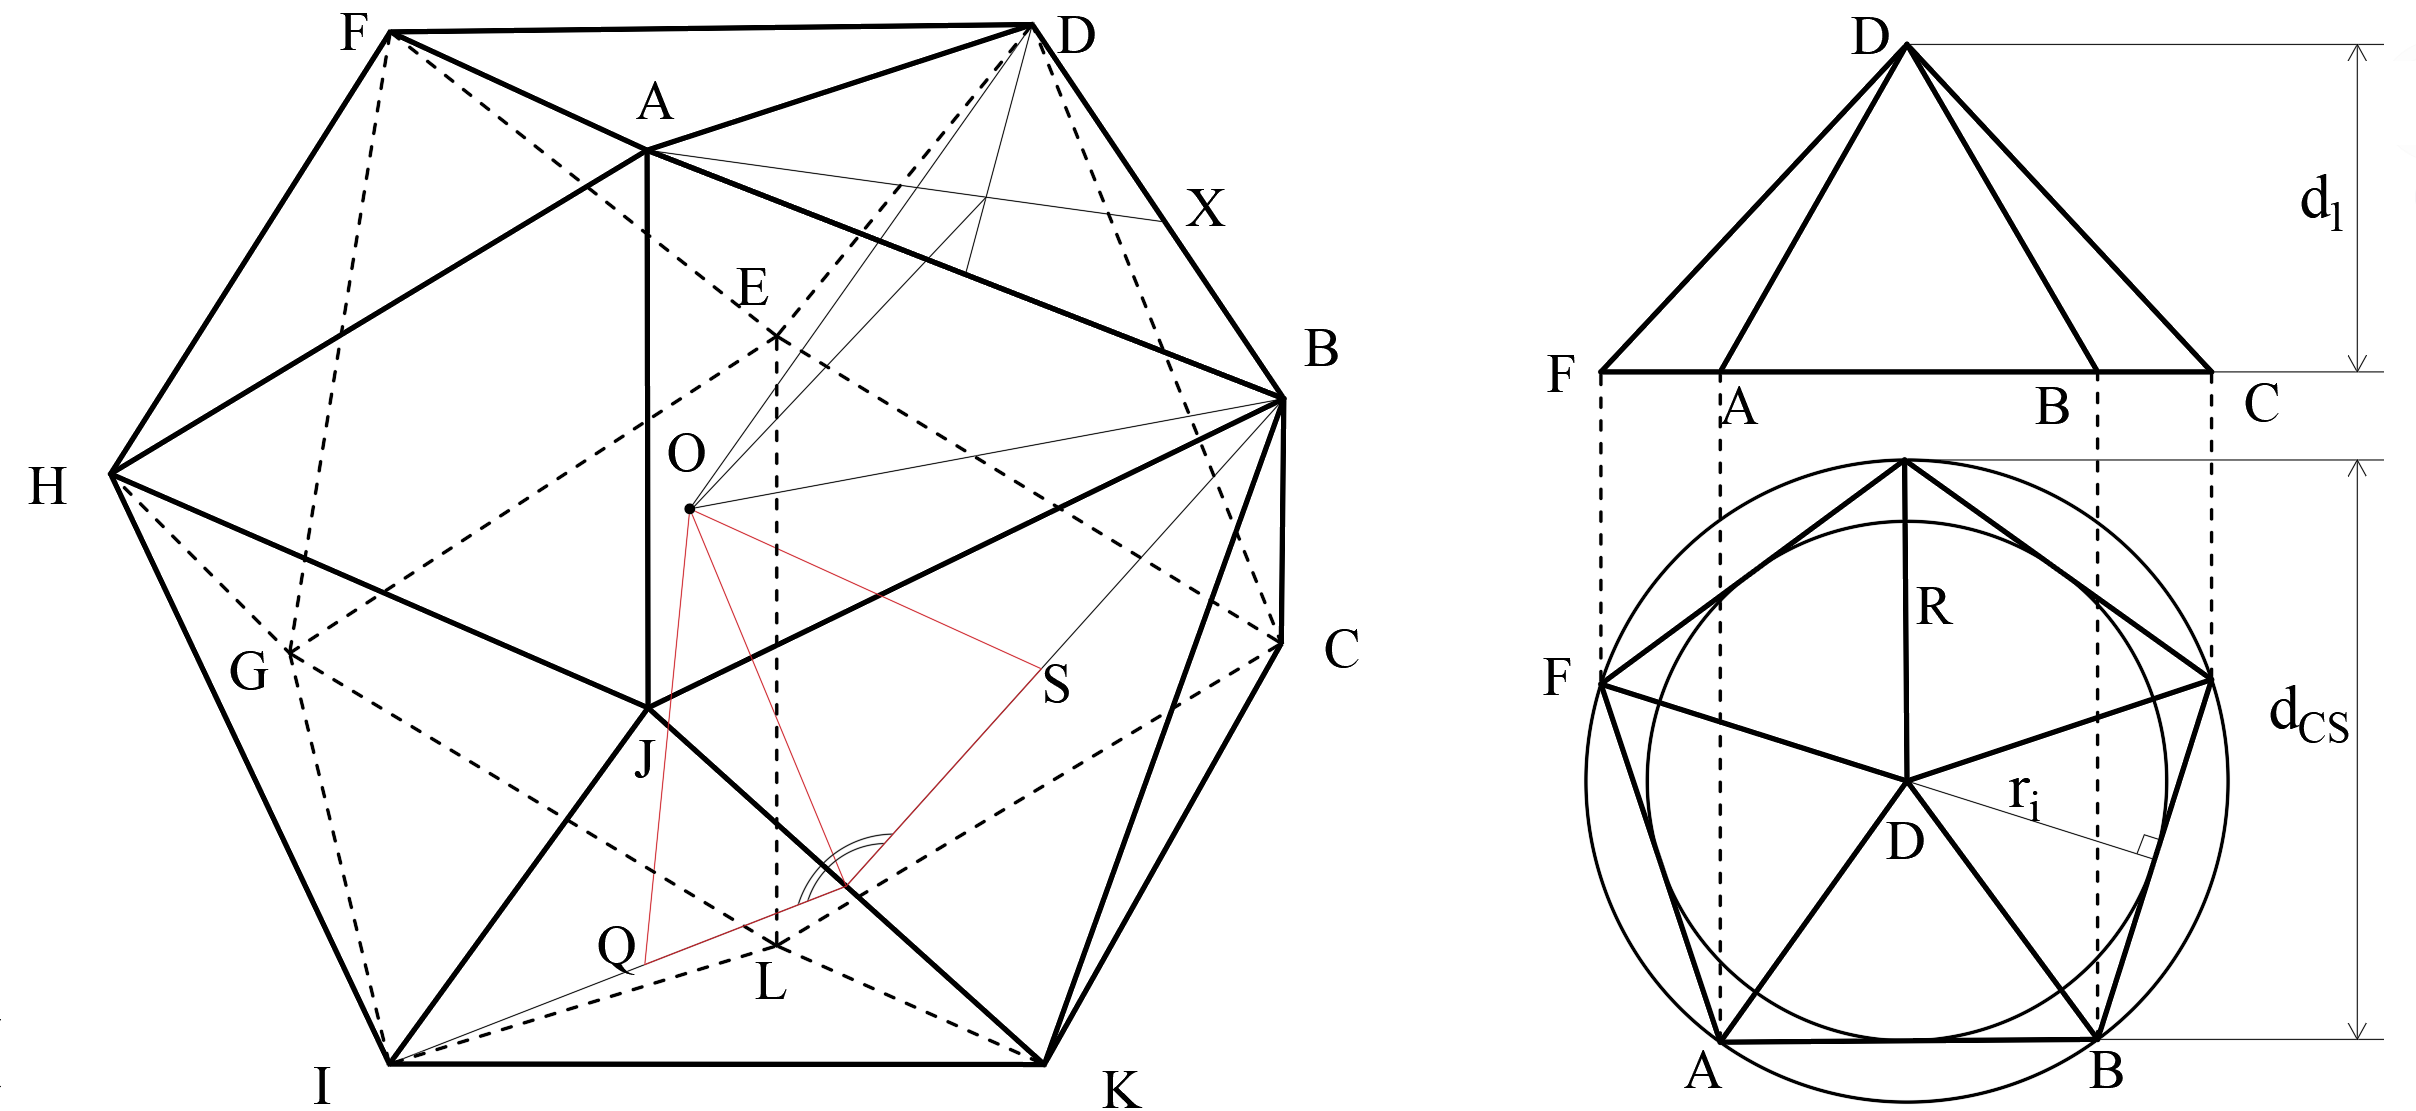
\includegraphics[width=\textwidth]{image/icosaGeo22.png}
%	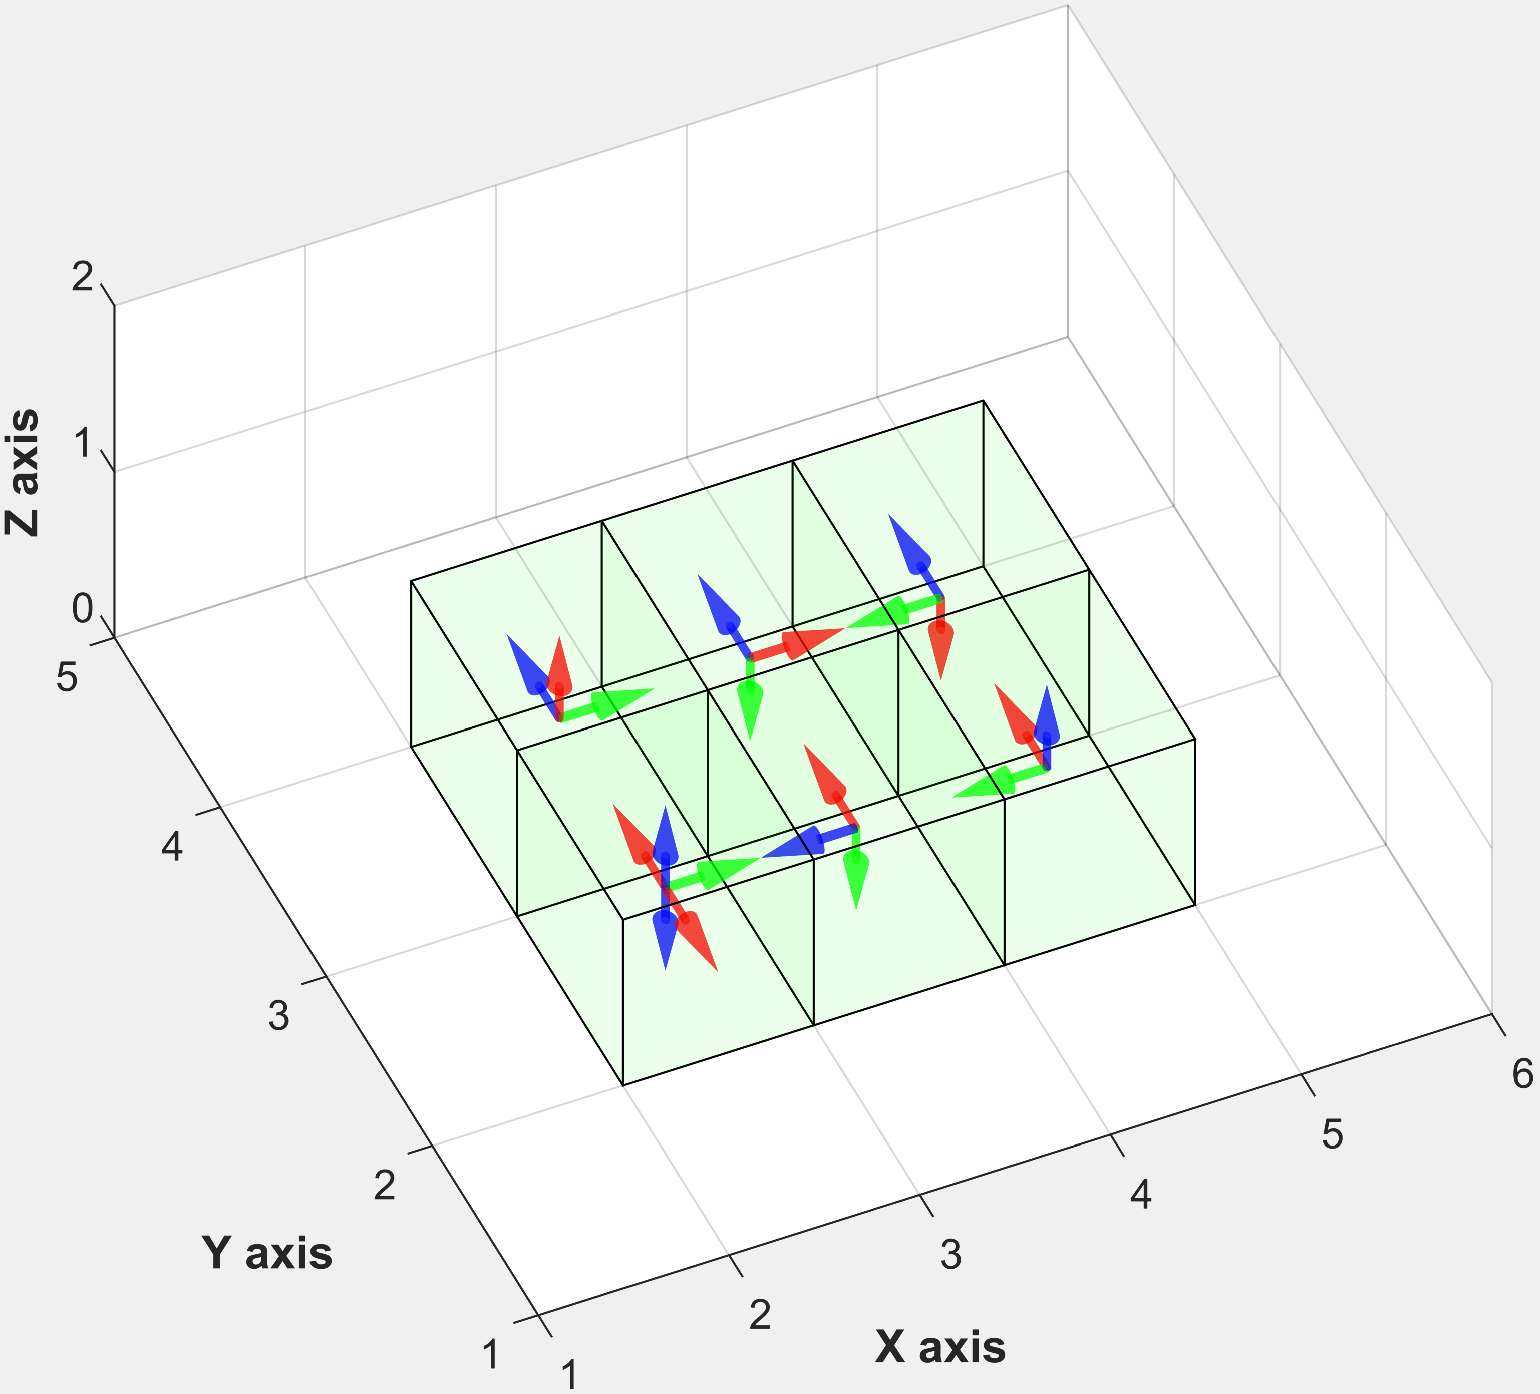
\includepdf[pages=-,pagecommand={},width=0.5\textwidth]{image/cubePath1.pdf}
	\caption{Icosahedron geometrical properties}
	\label{fig:icosaGeo2}
\end{figure}

\noindent At the right side of  the Figure \ref{fig:icosaGeo2}, the pentagon $ABCEF$ has circumcircle radius $R$, inscribed circle $r_i$, and the height $d_{CS}$ ($R+r_i$).
The golden ratio $\Phi$ (irrational number) has the value of $\frac{1+\sqrt{5}}{2}$ can be found by:
\begin{equation*} 
\label{icosa:eq1}
\begin{split}
\Phi & = \frac{OX}{XB} = \frac{OX}{\frac{1}{2}a}\\
\end{split}
\end{equation*}

%\sin(\angle XOB) & = \frac{XB}{OB} = \frac{\frac{1}{2}a}{\frac{\sqrt{\Phi^2+1}}{2}a}\\
%				 & = \frac{1}{\sqrt{\Phi^2 + 1}}\\
%\Rightarrow \angle{XOB} & = \arcsin{\frac{1}{\sqrt{\Phi^2 + 1}}}\\
%\Rightarrow \angle{DOB} & = 2\angle{XOB} = 2\arcsin{\frac{1}{\sqrt{\Phi^2 + 1}}}\\

\noindent Same as the case of cube's path planning algorithm, the initial step of rolling icosahedron is to find the rotation angle. 
The rotation angle is a supplementary of the $\angle{QRS}$. 
The line $OR$ is perpendicular to $QS$ and $OS = OQ = OM = r_i = \frac{\Phi^2}{2\sqrt{3}}a$. 
$BI$ is a diagonal of pentagon $BCLIJ$ and $\angle{QRS}=2\angle{ORS}$.\\

\noindent Otherwise, $OR=OX=\frac{1}{2}a\Phi$, and

\begin{equation*} 
\label{icosa:eq2}
\begin{split}
\angle{QRS} & = 2\angle{ORS}\\
\sin{\angle{ORS}} & = \frac{OS}{OR} = \frac{ \frac{\Phi^2}{2\sqrt{3}}a}{\frac{1}{2}a\Phi} = \frac{\Phi}{\sqrt{3}}\\
\Rightarrow \angle{QRS} & =2\arcsin{\frac{\Phi}{\sqrt{3}}}\\
\end{split}
\end{equation*}

\noindent To be more detail in Figure \ref{fig:icosaGeo5}, the rotation angle of icosahedron can be determined from the result of $\angle{QRS}$, as the following. 

\begin{equation*} 
\label{icosa:eq3}
\begin{split}
\beta & = \pi- \angle{QRS}\\
      & = \pi - 2\arcsin{\frac{\Phi}{\sqrt{3}}}\\
      & = \pi- \arccos{-\frac{\sqrt{5}}{3}}\\
\end{split}
\end{equation*}

\noindent To calculate the rotation axis for all the cases of the triangular surface contact, there are three axis such as $IJ$, $JK$, and $IK$ with the $3D$ coordinates as following.

%\begin{equation*} 
\begin{align*}
\label{icosa:eq4}
JK & = [a\quad  0\quad  0]\\
IJ & = [-\frac{1}{2}a\quad  (\frac{\sqrt{3}}{6}+\frac{\sqrt{3}}{3})a\quad  0]\\
IK & = [-\frac{1}{2}a\quad  -(\frac{\sqrt{3}}{6}+\frac{\sqrt{3}}{3})a\quad  0]
\end{align*}
%\end{equation*}

\begin{figure}[h]
\centering
	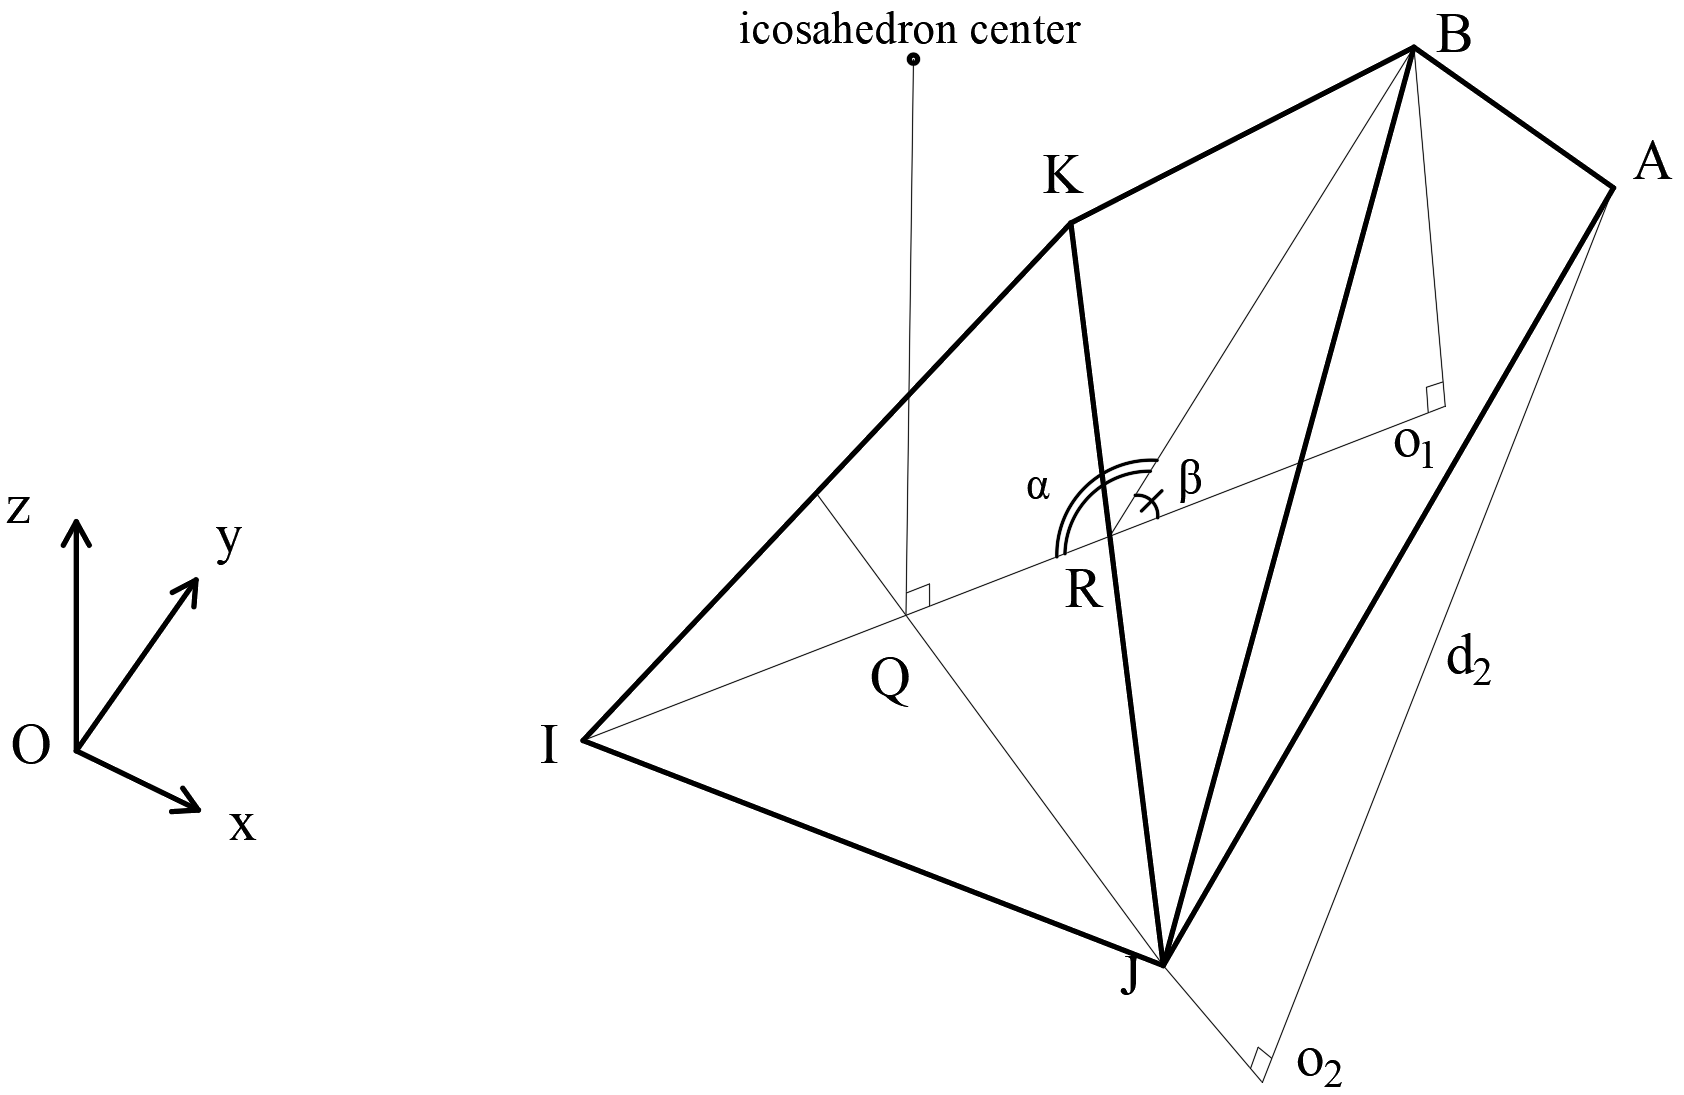
\includegraphics[width=0.5\textwidth]{image/icosaGeo55.png}
	\caption{Rotation angle and rotation axis}
	\label{fig:icosaGeo5}
\end{figure}

%
% ===================================
%
\noindent\uline{Path planning} 
Path planning of the regular icosahedron through rolling in known environment has initial coordinate at $[6.5, 5.5, 0]$ and the surface contact with red arrow points to bottom. 
The goal configuration with same as the initial coordinate has the contact surface with black arrow as shown in Figure \ref{fig:icosaPath1}. 
This figure shows the shortest path with the red line including 14 line segments. 
It means that the icosahedron rolled 14 times from the initial configuration to the goal configuration. 
The path can be seen more precisely from the top view in Figure \ref{fig:icosaPath2}.
The total length of this icosahedron path equals $14a\frac{\sqrt{3}}{3}$ (edge length of the octahedron is $a$).

\begin{center}
\begin{figure}[h]
\subfigure[The first shortest path of Icosahedron path rolling (Red line)]{
	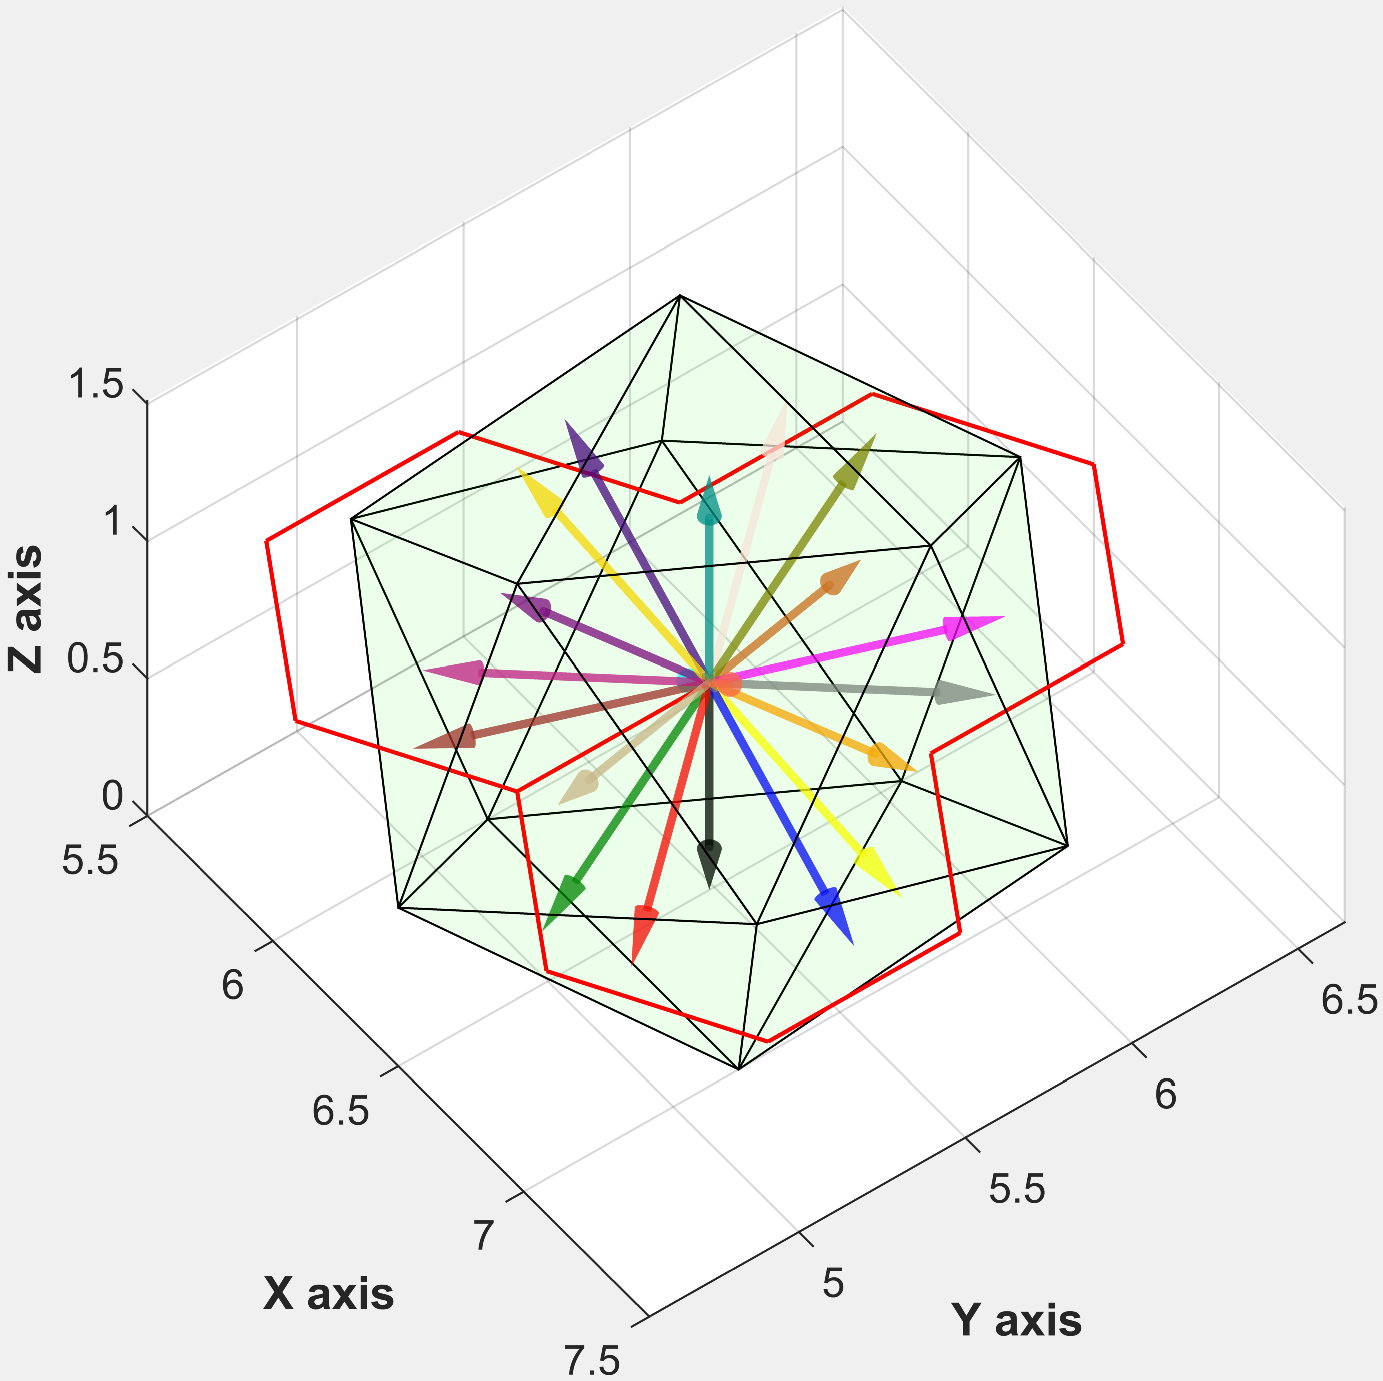
\includegraphics[width=0.5\textwidth]{image/icosaPath.pdf}
	\label{fig:icosaPath1}
	}
\hfill
\subfigure[The top view of path planning for Icosahedron]{
	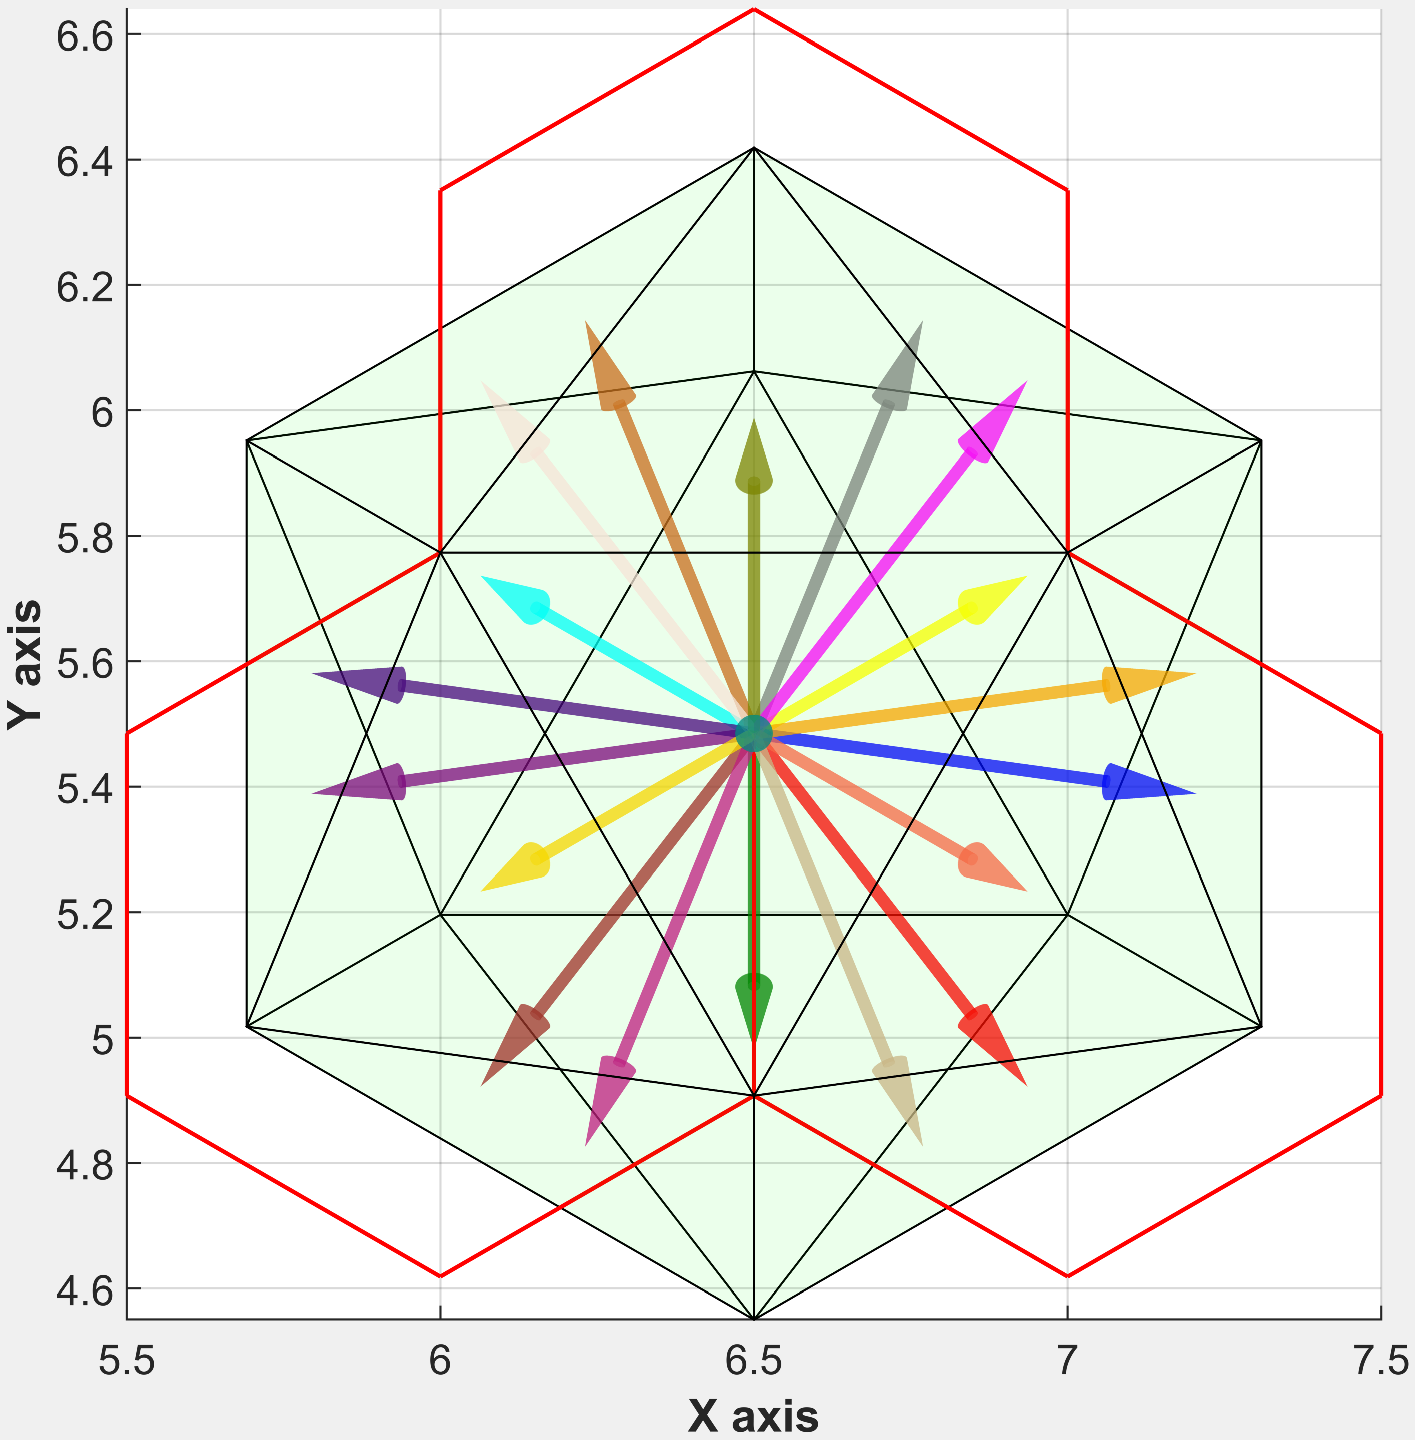
\includegraphics[width=0.5\textwidth]{image/icosaPathTopView.pdf}
	\label{fig:icosaPath2}
	}
\caption{Path of icosahedron rolling though edges}
\label{fig:icosaPaths}
\end{figure}
\end{center}
%
%
%%==================================================================================
%%                       Dodecahedron solid
%%==================================================================================
%%
%%
%%
%
\clearpage
\newpage
\subsection{Dodecahedron solid}

%\noindent\uline{Result}: 
%\begin{figure}[h]
%\centering
%	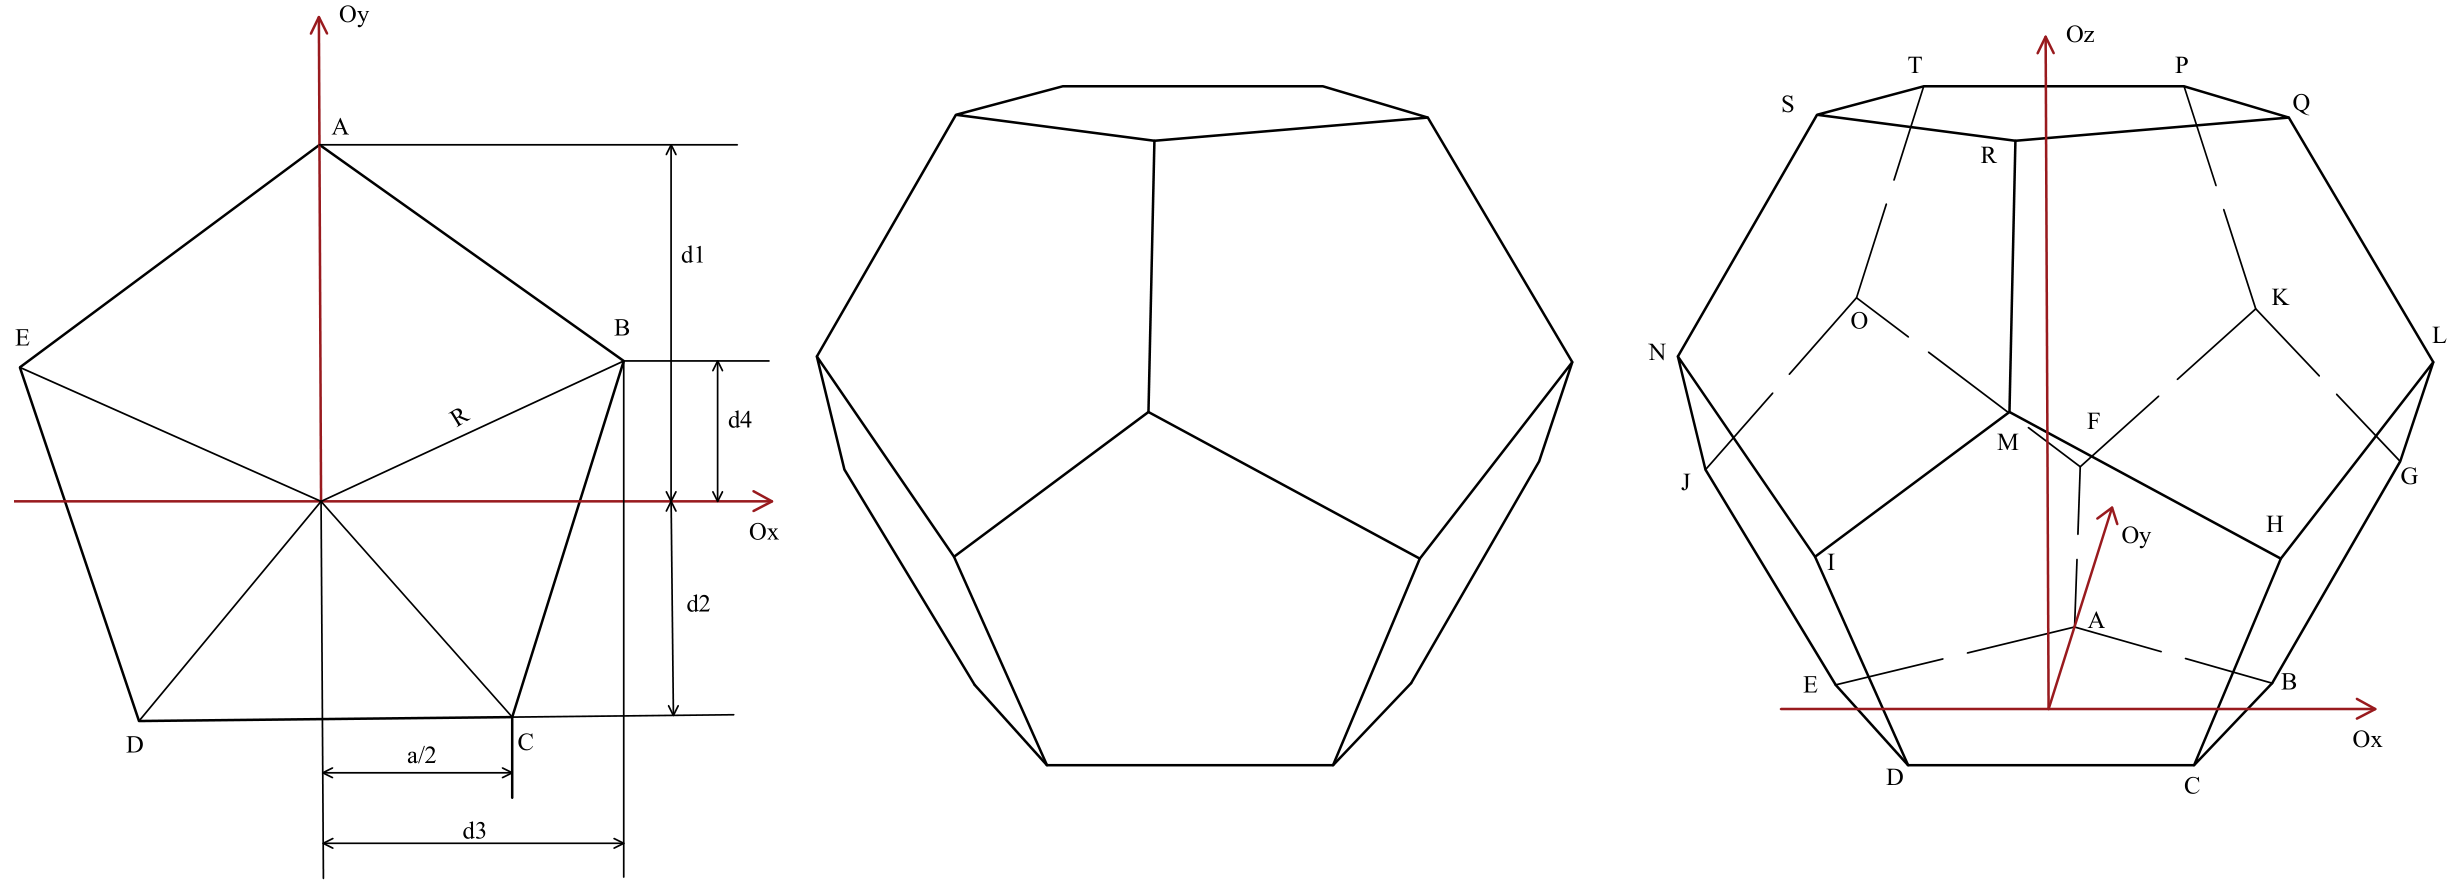
\includegraphics[width=1\textwidth]{image/dodecahedron1.png}
%	\caption{Shortest path of cube rolling}
%	\label{fig:dodecahedron1}
%\end{figure}

\noindent\uline{Properties}: 
An dodecahedron is constructed from twelve self-intersecting faces with the same pentagon shape. These faces meet at each vertex and there are total of twenty vertices in a dodecahedron as shown in Figure \ref{fig:dodecahedron2}.
%
From Eq. \ref{equa:eq1}, the great dodecahedron satisfy the Euler's formula ($V=20, F=12, E=30$).
%
It will be assumed that the coordinates $Oxyz$ lies on $ABCDE$ surface within $Oy$ through $A$ and $Oz$ perpendicular to $ABCDE$.
%
The 30 edges have the same length as $a$. It should be determined all the vertices' coordinates in the three dimensional system.
%
Figure \ref{fig:dodecahedron2} indicates the lengths of each vertex from $l_1$ to $l_4$ and the angles $\alpha_1$ to $\alpha_4$ which correspond to the five sides of a pentagon.

\begin{figure}[h]
\centering
	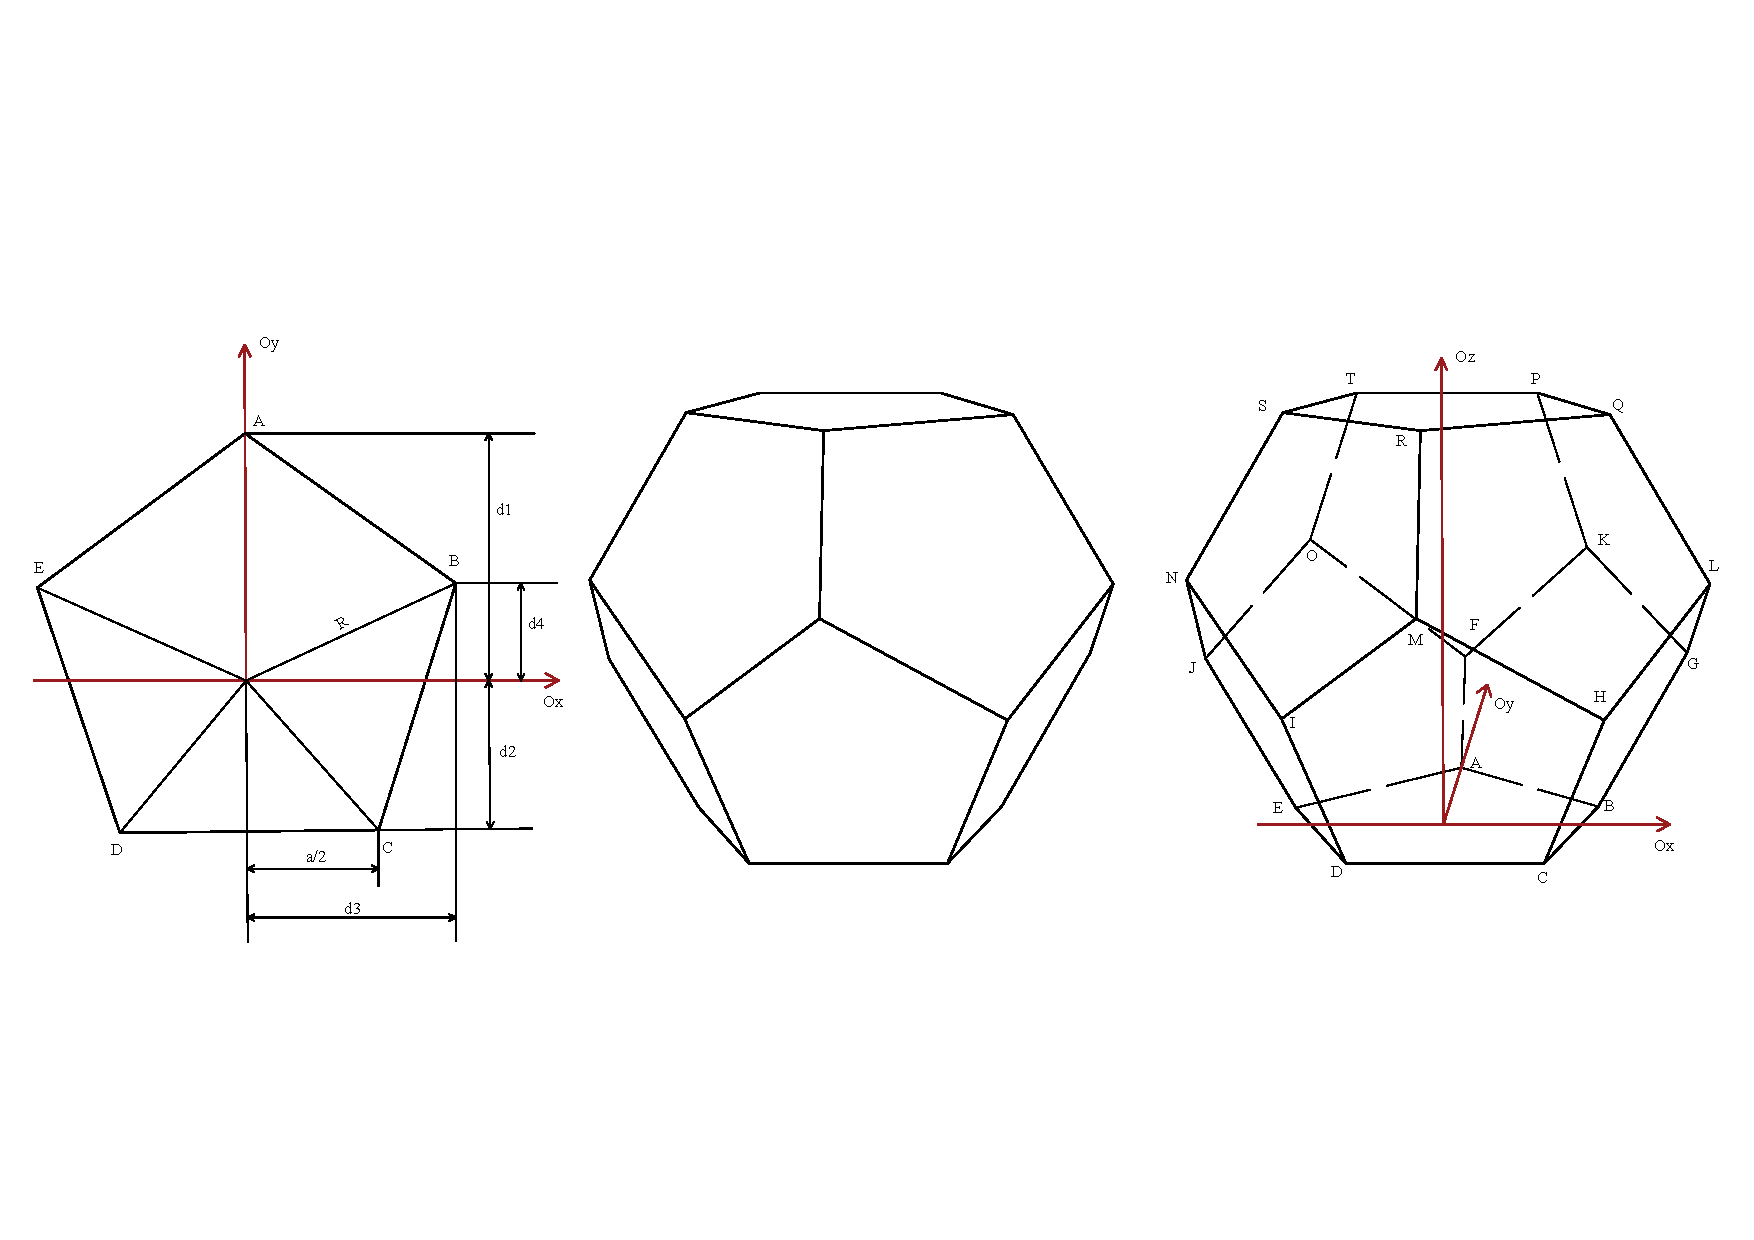
\includegraphics[width=1\textwidth]{image/dodecahedron2.pdf}
	\caption{Dodecahedron's vertices.}
	\label{fig:dodecahedron2}
\end{figure}

\noindent The path planning will implement on a surface but it will be considered in $3D$ spaces. 
Then, each vertex will be determined on $3D$ coordinates such as the vertex $A$ has coordinate with $[A_x A_y A_z]$. 
Based on the properties of pentagon, the angle $\alpha_1=\frac{2\pi}{5}$ and $\alpha_4=\frac{\pi}{5}$, 
because the angle between $Ox$ and $Oy$ is $\frac{\pi}{2}$, the sum of $\alpha_1$ and $\alpha_2$ is $\alpha_1 + \alpha_2 = \frac{\pi}{2}$. 
Then the other two angles $\alpha_2$ and $\alpha_3$ can be founded as below. 
\begin{equation*} 
\label{equa:eq0}
\begin{split}
\alpha_2 &= \frac{\pi}{2}-\alpha_1 = \frac{\pi}{2}-\frac{2\pi}{5} = \frac{\pi}{10}\\ 
\alpha_3 &= \alpha_1-\alpha_2 = \frac{2\pi}{5}-\frac{pi}{10} = \frac{3\pi}{10}
\end{split}
\end{equation*}

\noindent From Figure \ref{fig:dodecahedron2}(c), these labelled dimensions can be calculated as $l_1 = R_d = \frac{a}{2\sin{\alpha_4}}$ with $R_d$ is the circumradius of dodecahedron, $l_2 = l_1\cos{\alpha_4}$, $l_3 = l_1\cos{\alpha_2}$, and $l_4 = l_1\sin{\alpha_2}$. 
The golden ratio $\Phi$ with the value of $\frac{1+\sqrt{5}}{2}$ which is the length of the diagonal of a square with $1$ unit length of sides is used to calculate the circumscribed sphere radius of dodecahedron. It can be assumed that the dodecahedron has the length $a$, the radius of an inscribed sphere ($r_i$) and the circumscribed sphere radius ($r$) are shown as below.
\begin{equation*}
\begin{split}
r_i &= \frac{a}{20}\sqrt{10(25+11\sqrt{5})}\\
r &= a\frac{\sqrt{3}}{2}\frac{1+\sqrt{5}}{2}
\end{split}
\end{equation*}
\noindent In the path-finding through rolling, the proposed algorithm focuses on the transformation and translation of $20$ vertices of a dodecahedron. 
Although rolling dodecahedron's faces on $2D$ surface, the bottom surface which integrates to the $Oxy$ will contact to the surface in the three dimensional space. 
This condition expresses the $Oz$ dimension of all the $(A,B,C,D,E)$ vertices which equal to $0$ or $A_z = B_z = C_z = D_z = E_z = 0$. 
Then, 
\begin{equation*} 
\label{equa:eq01}
\begin{split}
P_z = Q_z = R_z = S_z = T_z &= 2.r_i \\
							&= \frac{a}{10}\sqrt{10(25+11\sqrt{5})}
\end{split}
\end{equation*}
\noindent It can be seen that the distance $|AF|$ is $a$ and the distance $|BF|$ is $2l_3$. Using the distance properties and squaring the results give:
\begin{equation*} 
\label{dodeca:eq1}
\begin{split}
AF^2 & = a^2 = (A_x-F_x)^2 + (A_y-F_y)^2 + (A_z-F_z)^2 \\
BF^2 & = (2l_3)^2 = (B_x-F_x)^2 + (B_y-F_y)^2 + (B_z-F_z)^2
\end{split}
\end{equation*}

\noindent Figure \ref{fig:dodecahedron2}(d) shows that $A_x = F_x = 0$, $A_y = l_1$, $B_y = l_4$, $B_x = l_3$, $A_z = B_z$. Define $l_5=A_z-F_z$, the relations of these equations are:
\begin{equation*} 
\label{dodeca:eq2}
\begin{split}
a^2 & = (F_y-l_1)^2 + l_5^2\\
(2l_3)^2 & = (F_y-l_4)^2 + l_5^2 + l_3^2
\end{split}
\end{equation*}

\noindent Solving $F_y$ and $l_5$ gives:
\begin{equation*} 
\label{dodeca:eq3}
\begin{split}
F_y & = \frac{a^2-(2l_3)^2-(l_1^2-l_3^2-l_4^2)}{2(l_4-l_1)} \\
l_5 & = \frac{1}{\sqrt{2}}\sqrt{a^2+(2l_3)^2-(F_y-l_1)^2-(F_y-l_4)^2-l_3^2}
\end{split}
\end{equation*}

\noindent From these above equations, all the vertices can be determined and stored in a $3D$ matrix. 
In every single position, another matrix stores the edge's contact and the rotated-direction. 
Using these information with the rotation matrix $R_{\hat{\omega}(\theta)}$, the path planning algorithm will generate a new matrix for the dodecahedron at new position after rolling through its edge.\\
%
%
%===========================Path Planning=============================

\noindent\uline{Path Planning}: As mentioned in Section \ref{sec:Algorithm}, the dodecahedron can roll on the two grid types. 
The simple case has a gap at the connection between three regular pentagons as shown in Figure \ref{fig:dodecaGrid}. 
%
In this paper, we do not apply the proposed algorithm to find the path of dodecahedron with rolling on the case of overlaps between four pentagons. 
This overlap grid is complicated environment which can not guarantee to generate paths with proposed algorithm. 
%
In the case of gird with gaps (Figure \ref{fig:dodecaGrid}), attaching other five pentagons generates five $\ang{36}$ gaps from a regular pentagon. 
The six pentagons has a shape of large pentagon and the cycle of attaching more five larger pentagons will shape a grid of pentagons.
%
\begin{figure}[H]
\centering
	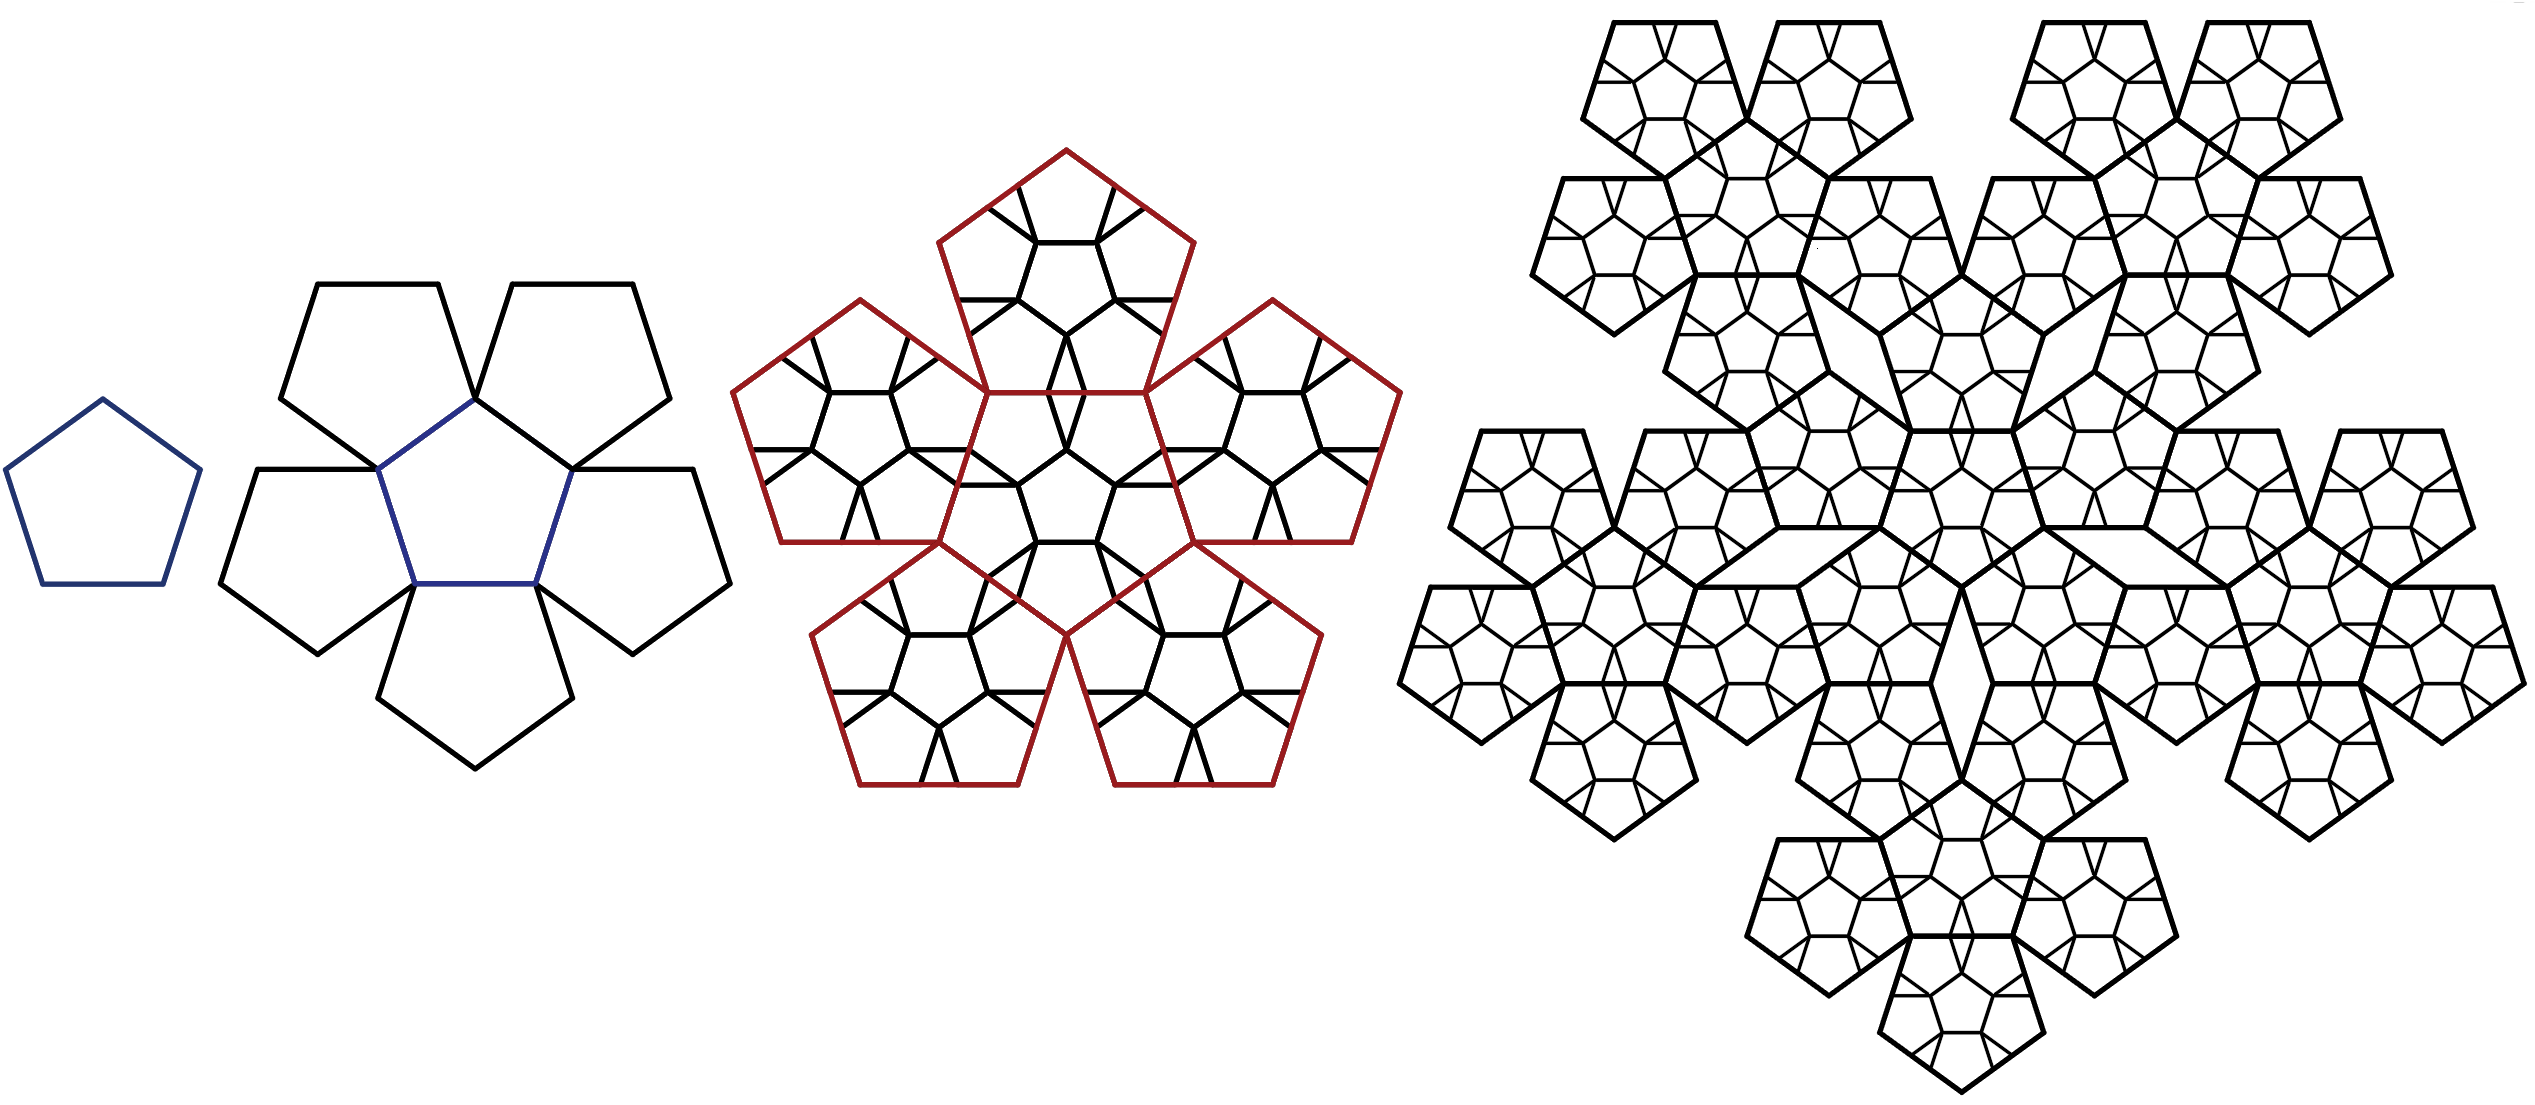
\includegraphics[width=\textwidth]{image/dodecaGrid.png}
	\caption{Initial dodecahedron grid with gaps}
	\label{fig:dodecaGrid}
\end{figure}
\noindent The rotation angle of dodecahedron on the above grid equals 
to $\pi-\arccos{(\frac{-\sqrt{5}}{5})}$. 
One of the closed-paths shown in Figure \ref{fig:dodecaPath} is initialized for both the initial and goal coordinates with $[3.0\ 2.25\ 0.0]$.
Each step of the rolling dodecahedron generates a new dodecahedron which has a distance of $d=2l_2$ from the previous coordinate. 
From Figure \ref{fig:dodecahedron2}b, the distance $d_d$ can be determined as following.
\begin{equation*} 
\label{dodeca:eq4}
\begin{split}
l_2 & = l_1\cos{\alpha_4}\\
    & = \frac{a}{2\sin{\alpha_4}}\cos{\alpha_4}\\
    & = \frac{1}{2}a\cot{\alpha_4}\\
\rightarrow d_d & = a\cot{\alpha_4}
\end{split}
\end{equation*}

\noindent Then, the total length of the first path with the red line equals $15a\cot{\alpha_4}$ as shown in Figure \ref{fig:dodecaPath}.\\
%\begin{figure}[h]
%\centering
%	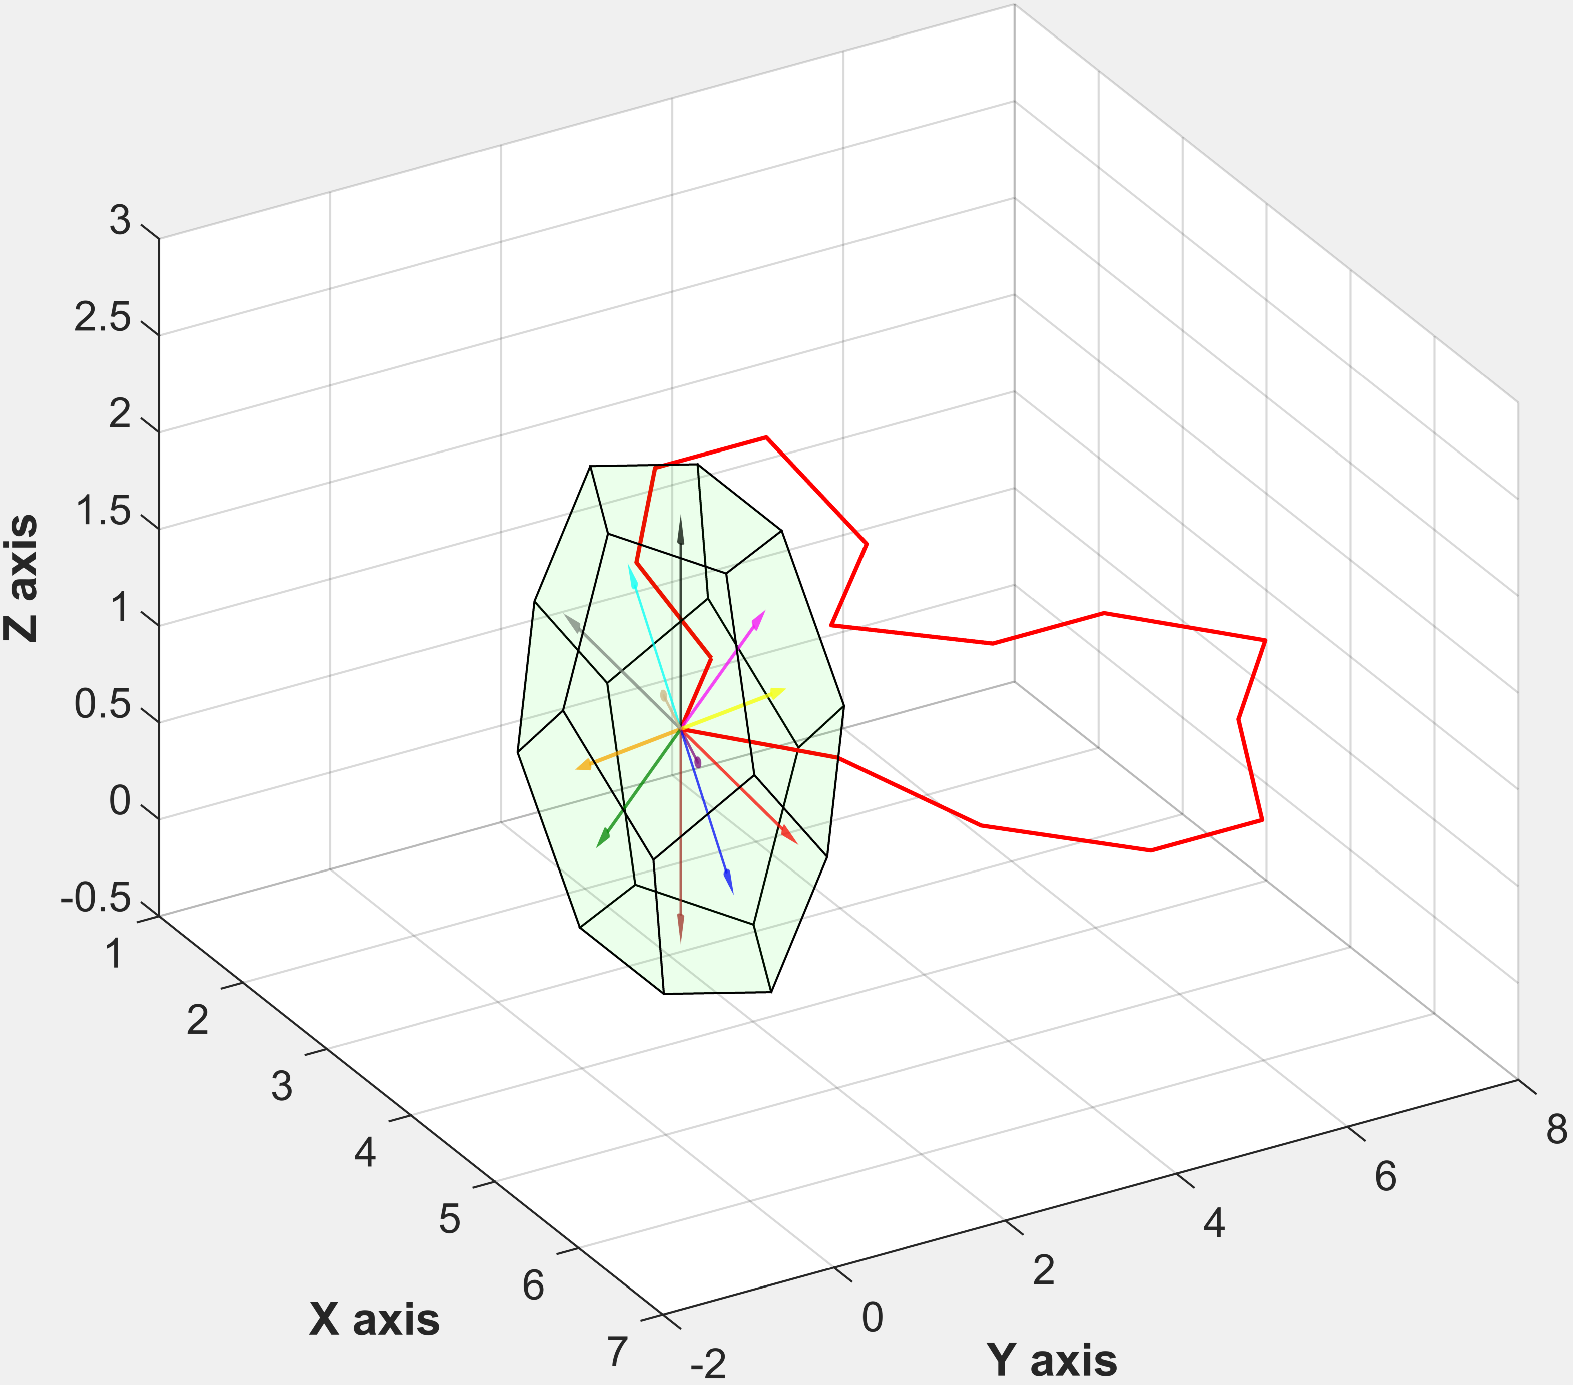
\includegraphics[width=\textwidth]{image/dodecaPath1.pdf}
%	\caption{The rolling path of dodecahedron at an coordinate with $[3.0\ 2.25\ 0.0]$}
%	\label{fig:dodecaPath1}
%\end{figure}

\begin{center}
\begin{figure}[h]
\subfigure[The top view of the grid for the gap case]{
	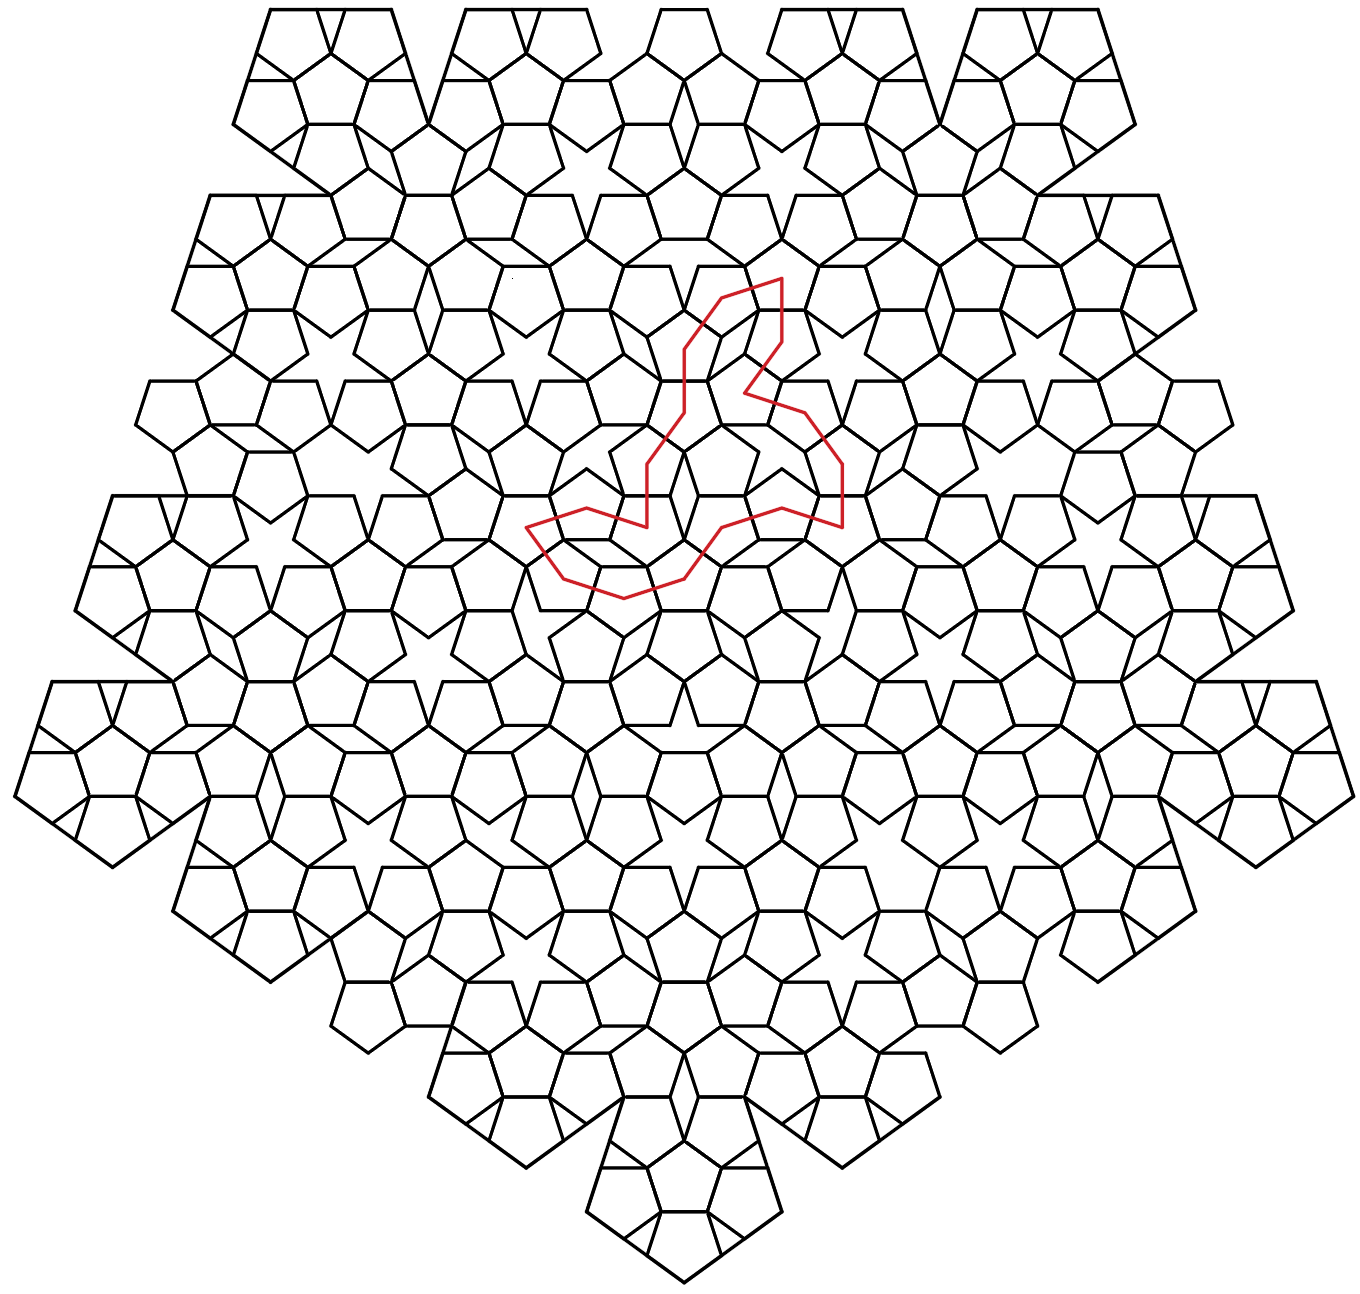
\includegraphics[width=0.45\textwidth]{image/dodecaGridPath1.png}
	\label{fig:dodecaGridPath1}
	}
\hfill
\subfigure[Simulation result in Matlab]{
	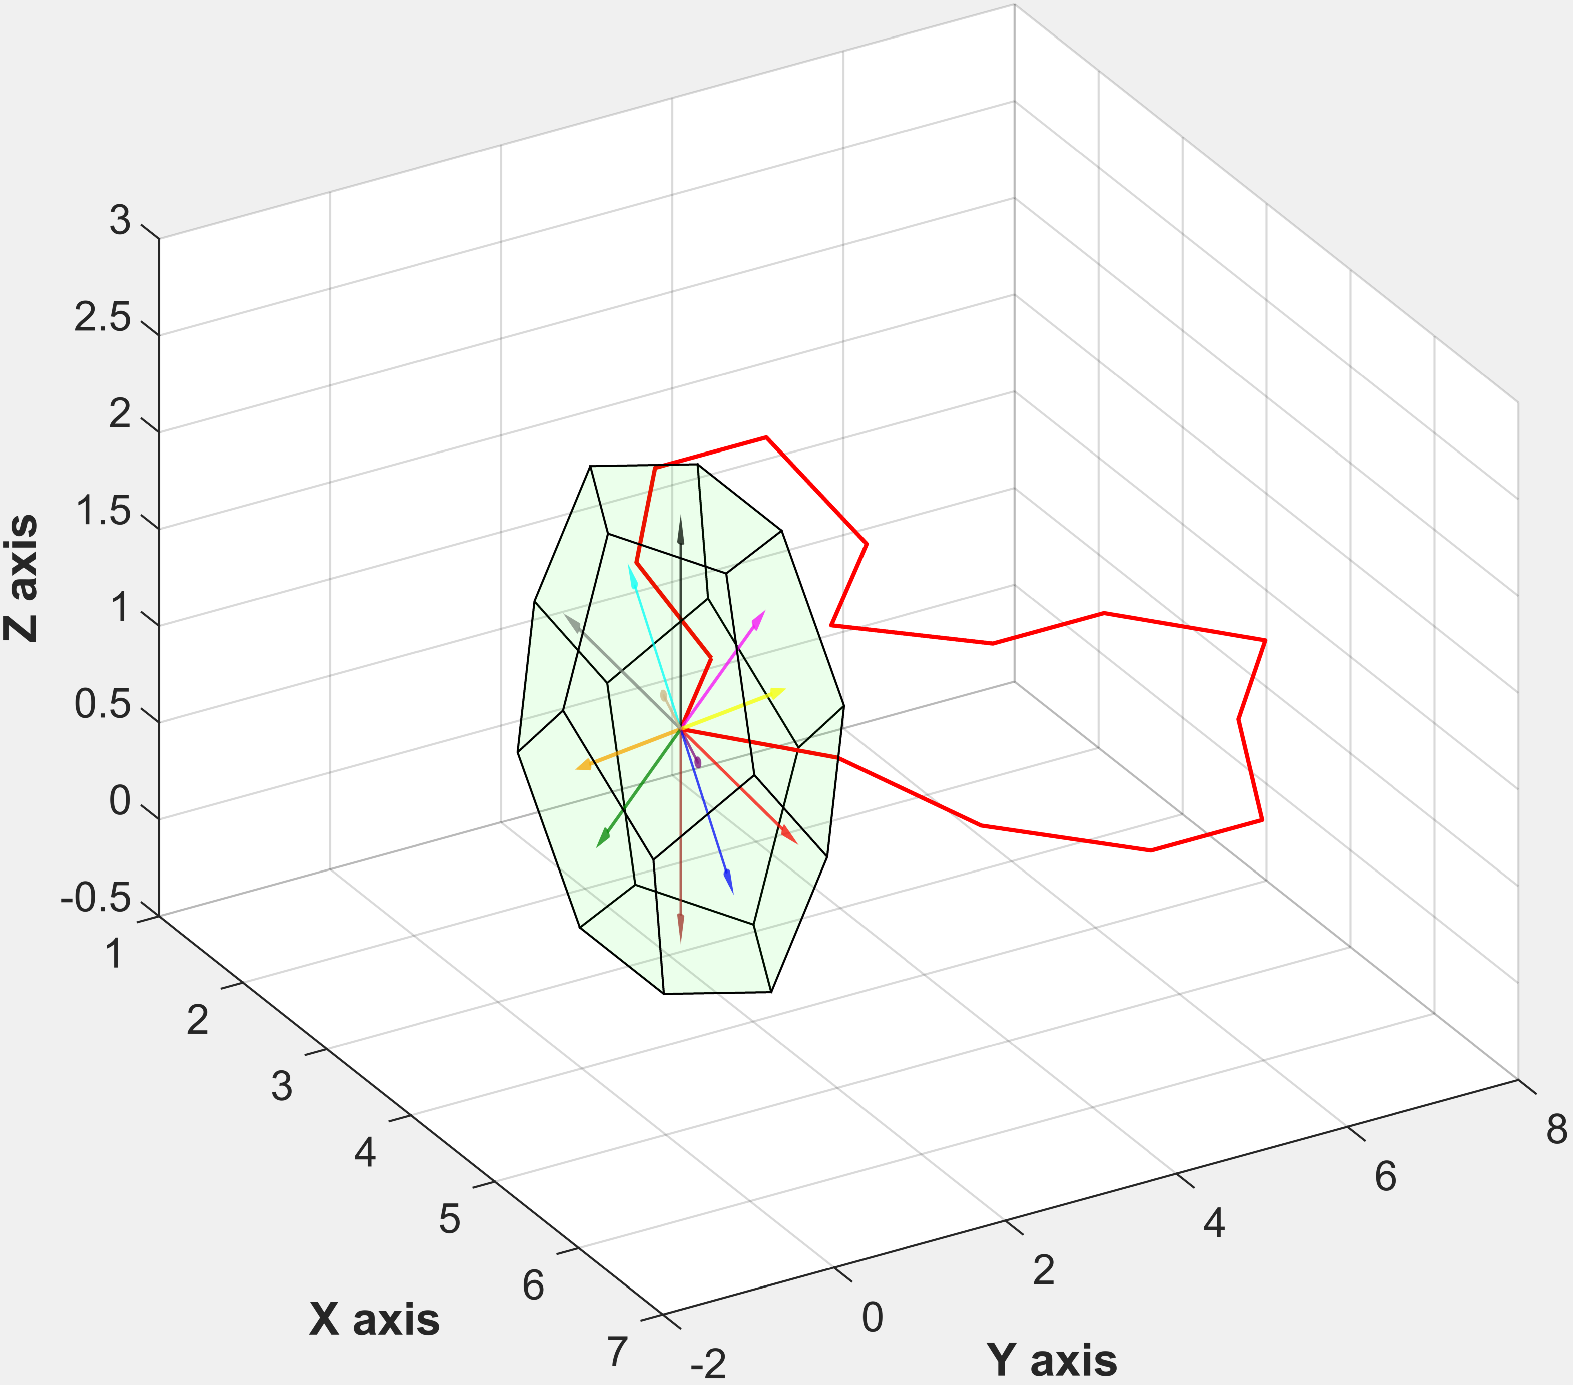
\includegraphics[width=0.5\textwidth]{image/dodecaPath1.pdf}
	\label{fig:fig:dodecaPath1}
	}
\caption{The rolling path of dodecahedron at an coordinate with $[3.0\ 2.25\ 0.0]$}
\label{fig:dodecaPath}
\end{figure}
\end{center}

\noindent According to the simulation results, implementing the proposed algorithm for other four types of platonic solids including cube, tetrahedron, octahedron, and icosahedron is more effective than for the dodecahedron case. 
%
The closed-path planning algorithm through rolling contact for the case of dodecahedron is complex due the various initial environments. 
%
Executing the algorithm is no guarantee of path-finding results with the other cases of overlap grid.
%%==================================================================================
%%
\subsection{Result comparisons}
%%
%%
\noindent \uline{Extension case}: The proposed algorithm in this study can be applied for the case study of long distance between the initial and goal configurations. 
Figure \ref{fig:cubeLongDist} shows an example with two different paths.
The closed-path planning algorithm is added to the point-to-point algorithm based on rolling in order to find the path from start point to the goal point. 
Assume that the initial configuration is at $S_1$ and the goal configuration is at $S2$.
At the stage of point-to-point planning, the red line segment $S_1S_2$ shows the shortest distance from start position to goal position and the path can be generated along this red line. 
After achieving the goal position without considering the orientation, the cube updates this configuration as a new start configuration.
Then, the proposed closed-path planning algorithm will implement with this updated configuration to achieve the original goal configuration.
\\ 

\begin{figure}[H]
\subfigure[Path 1]{
	\includegraphics[width=0.5\linewidth]{image/cubeCase2Path1.jpg} 
	\label{fig:cubeLongDistPath1}}
\subfigure[Path 2]{
	\includegraphics[width=0.5\linewidth]{image/cubeCase2Path2.jpg}
	\label{fig:cubeLongDistPath2}}
\caption{Caption for this figure with two images}
\label{fig:cubeLongDist}
\end{figure}

%%
%%
%%
%%

\noindent \uline{Execution time}:
As can be seen in Figure \ref{fig:cubeLongDist}, the point-to-point path planning in the first stage generates two same path from $S_1S_2$. In the second stage, the closed path planning algorithm finds two different closed-paths. The first closed-path has $16$ steps while the second closed-path has $18$ steps of rolling to achieve the goal.
The execution times are shown in Table \ref{tab:timeCubeExtension}. The shorter path has less time to implement the closed-path planning algorithm than the longer path with more steps.\\

%https://www.tablesgenerator.com/
\begin{table}[H]
\caption{The execution times of two paths of the rolling cube shown in Figure \ref{fig:cubeLongDist}}
\centering
\begin{tabular}{cccll}
\cline{1-3}
\multicolumn{1}{|c|}{Execution Time (ms)}          & \multicolumn{1}{c|}{Path 1} & \multicolumn{1}{c|}{Path 2} &  &  \\ \cline{1-3}
\multicolumn{1}{|c|}{Poin-to-point} & \multicolumn{1}{c|}{0.25}    & \multicolumn{1}{c|}{0.25}    &  &  \\ \cline{1-3}
\multicolumn{1}{|c|}{Proposed algorithm} & \multicolumn{1}{c|}{2.02} & \multicolumn{1}{c|}{2.34} &  &  \\ \cline{1-3}
\multicolumn{1}{l}{}                & \multicolumn{1}{l}{}        & \multicolumn{1}{l}{}        &  & 
\end{tabular}
\label{tab:timeCubeExtension}
\end{table}


\noindent Considering the execution times for the five types of platonic solids, Table \ref{tab:twoPathsPlatonics} shows that the proposed algorithm runs in a short time to find the closed-paths for the rolling cube and tetrahedron. 
The longer execution times depend on the complex geometry of each polyhedron. In this case, the running time of the closed-path planning for the icosahedron implements extensively. \\


\begin{table}[H]
\centering
\caption{The execution times of the first two paths are found for the platonic solids}
\begin{tabular}{|c|c|c|c|c|c|}
\hline
Execution Time (ms) & Cube & Tetrahedron & Octahedron & Icosahedron & Dedecahedron \\ \hline
First path          & 4.15 & 5.02 & 48.45 & 135.34 & 89.74 \\ \hline
Second path         & 4.15 & 5.02 & 62.78 & 179.35 & N/A          \\ \hline
\end{tabular}
\label{tab:twoPathsPlatonics}
\end{table}